%%% Dateikodierung: UTF-8
%%% äöüÄÖÜß  <-- keine deutschen Umlaute hier? UTF-faehigen Editor verwenden!

%%% Magic Comments zum Setzen der korrekten Parameter in kompatiblen IDEs
% !TeX encoding = utf8
% !TeX program = pdflatex 
% !TeX spellcheck = de_DE
% !BIB program = biber
\documentclass[master,german,smartquotes]{hgbthesis}
% Zulässige Optionen in [..]: 
%    Typ der Arbeit: 'diploma', 'master' (default), 'bachelor', 'internship' 
%    Hauptsprache: 'german' (default), 'english'
%    Option zur Umwandlung in typografische Anführungszeichen: 'smartquotes'
%    APA Zitierstil: 'apa'
%%%-----------------------------------------------------------------------------

\RequirePackage[utf8]{inputenc} % bei Verw. von lualatex oder xelatex entfernen!

\graphicspath{{images/}}  % Verzeichnis mit Bildern und Grafiken
\logofile{logo}           % Logo-Datei: images/logo.pdf (kein Logo: \logofile{})
\bibliography{references} % Biblatex-Literaturdatei (references.bib)

%%%-----------------------------------------------------------------------------
% Angaben für die Titelei (Titelseite, Erklärung etc.)
%%%-----------------------------------------------------------------------------

\title{Best-Practice-Ansätze zur Umsetzung von technischen IT-Sicherheitsanforderungen an eine Bank in Österreich}
\author{Philipp Gigler, BSc MSc}
\programname{Information Security Management}

%\programtype{Fachhochschul-Bachelorstudiengang} % auswählen/editieren
\programtype{Fachhochschul-Masterstudiengang}

\placeofstudy{Hagenberg}
\dateofsubmission{2022}{07}{15} % {YYYY}{MM}{DD}

\advisor{FH-Prof. Dr. Harald Lampesberger, MSc} % optional

%\strictlicense % restriktive Lizenz anstatt Creative Commons (nicht empfohlen!)

%%%-----------------------------------------------------------------------------
\begin{document}
%%%--------------------------------------------------------------------------

%%%-----------------------------------------------------------------------------
\frontmatter                                       % Titelei (röm. Seitenzahlen)
%%%-----------------------------------------------------------------------------

\maketitle
\tableofcontents

%%\chapter{Vorwort} 	% engl. Preface
 % Ein Vorwort ist optional
\chapter{Kurzfassung}
Aufgrund der steigender Bedrohung von Cyberangriffen auf IT-Systemen stellen Aufsichtsbehörden verstärkt Vorgaben an die IT-Sicherheit von Unternehmen. Ein Cyberangriff oder ein Ausfall von IT-Infrastrukturkomponenten kann einen erheblichen finanziellen und reputationstechnischen Schaden für Unternehmen darstellen. Vor allem die Sicherheit von Banken und anderer Finanzdienstleister stehen verstärkt im Fokus von Aufsichtsbehörden. Für Finanzinstitute gilt es einerseits die technische Sicherheit der eigenen IT-Umgebung zu erhöhen um Angriffe zu vereiteln und andererseits den unterschiedlichen Anforderungen von Aufsichtsbehörden nachzukommen. Die vorliegende Arbeit beschäftigt sich mit Anforderungen von Aufsichtsbehörden an die technische IT-Sicherheit von Banken in Österreich. Im Zuge dessen werden für die Ausarbeitung relevante Richtlinien erhoben und die Vollständigkeit der untersuchten Richtlinien mittels Peer Reviews sichergestellt. Die Richtlinien werden in weiterer Folge und auf technisch umzusetzende Sicherheitsanforderungen hin analysiert. Diese Sicherheitsanforderungen werden kategorisiert und mögliche technische Umsetzungen abgeleitet. Es wird der Frage nachgegangen, ob sich diese technischen Sicherheitsanforderungen auch mittels bereits etablierter Best-Practice-Ansätze umsetzen lassen. Ziel der vorliegenden Arbeit ist es einen Überblick über technische IT-Sicherheitsanforderungen an Banken in Österreich zu geben, die jeweilig adressierten Themenbereiche zu erörtern und mögliche Maßnahmen zur Umsetzung darzulegen.		
\chapter{Abstract}
Due to the increasing threat of cyber attacks on IT systems, regulatory authorities are increasingly imposing requirements on companies' IT security. A cyber attack or a failure of IT infrastructure components can cause considerable financial and reputational damage to companies. In particular, the security of banks and other financial service providers is increasingly in the focus of supervisory authorities. On the one hand, financial institutions need to increase the technical security of their own IT environment in order to thwart attacks, and on the other hand, they need to meet the various requirements of supervisory authorities. This paper deals with the requirements of supervisory authorities for the technical IT security of banks in Austria. In the course of this work, relevant guidelines are collected and the completeness of the examined guidelines is ensured by means of peer reviews. The guidelines are then analyzed in terms of technical security requirements that need to be implemented. These security requirements are categorized and possible technical implementations are derived. The question of whether these technical security requirements can also be implemented using established best-practice approaches is investigated. The aim of this paper is to provide an overview of technical IT security requirements for banks in Austria, to discuss the respective topics addressed and to present possible measures for implementation.			

%%%-----------------------------------------------------------------------------
\mainmatter                             % Hauptteil (ab hier arab. Seitenzahlen)
%%%-----------------------------------------------------------------------------

\setlength{\parindent}{0em} 

%**********************************************************************************
% Kapitel Einleitung
%**********************************************************************************
\chapter{Einleitung}
\label{cha:einleitung}
Das Thema IT-Sicherheit wird für Unternehmen immer essentieller. Speziell der Banken-Sektor stellt ein lukratives Ziel für Angreifer dar, da Banken als als \glqq{}Verteilzentren\grqq{} weltweiter Finanztransaktionen dienen. In den IT-Systemen von Banken werden Geldtransaktionen aus aller Welt gespeichert und Kundendaten verarbeitet. 
Laut einer Studie der \glqq{}Boston Consulting Group\grqq{} (BCG\footnote{https://www.bcg.com}) treffen Cyberattacken Finanzdienstleister 300-Mal häufiger als Unternehmen aus anderen Sparten. Trotz dieser Tatsache sind viele Finanzdienstleister nicht genug auf Cyberangriffe und deren Folgen vorbereitet. 
Unterschiedliche Faktoren wie der steigende Konkurrenzdruck und die Etablierung von nicht-traditionellen Marktteilnehmern und Fintech-Unternehmen führen dazu, dass der Bereich der IT-Sicherheit bei Finanzdienstleistern oft von Einsparungen betroffen ist. \autocite{Zakrzewsk2019} 
\bigbreak
Ein Cyberangriff oder ein Ausfall von IT-Infrastrukturkomponenten kann zu einem erheblichen finanziellen und reputationstechnischen Schaden für Finanzdienstleister und deren Partner führen. Ein weiterer möglicher Schaden eines Cyberangriffs ist der Verlust des Vertrauens der Kunden in das betroffene Finanzinstitut. Aus diesem Grund existieren für Finanzinstitute weitreichende Vorschriften betreffend der Sicherheit von IT-Systemen. \cite{EY2021} 
\bigbreak
Das Risiko eines Cyberangriffs, etwa auf die Infrastruktur eines Finanzdienstleisters, wird um einen weiteren Faktor verschärft. Es kann vorkommen, dass es Finanzdienstleistern nicht möglich ist, eine eigene IT-Infrastruktur zu betreiben. Aus diesem Grunde können unterschiedliche Aufgaben an Dritte ausgelagert werden um Kosten zu sparen und somit einen Wettbewerbsvorteil zu lukrieren. Anstatt beispielsweise die notwendige IT-Infrastruktur selbst zu betreiben, nötige Prozesse zu etablieren und Mitarbeiter zu beschäftigen, werden diese Aufgaben von spezialisierten Dienstleistern erbracht. Durch diese Auslagerung entsteht für den Finanzdienstleister eine neue Art von Risiko. Neben dem tatsächlichen Ausfall von Hard- oder Software oder einem Angriff auf die IT-Infrastruktur wird der gesamte Dienstleister zu einem Risiko. Dieses Risiko besteht, wenn der Dienstleister seine Leistungen nicht oder nicht ausreichend erbringt, oder selbst Opfer eines Cyberangriffs wird. \autocite{Presse2019} 
\bigbreak
Aufgrund der steigenden Relevanz von IT-Sicherheit im Zuge von Auslagerungen hat die \glqq{}Europäische Bankenaufsichtsbehörde\grqq{} (EBA\footnote{https://www.eba.europa.eu}) im Jahr 2019 eine Leitlinie zum Umgang mit Auslagerungsrisiken veröffentlicht (EBA/GL/2019/02) \autocite{eba_leitlinien_konvergenzkriterien}. Parallel dazu wird auf europäischer Ebene an einer Harmonisierung regulatorischer Anforderungen an die IT-Sicherheit von Finanzunternehmen in Europa gearbeitet. Die \glqq{}Europäische Aufsichtsbehörde für das Versicherungswesen und die betriebliche Altersversorgung\grqq{} (EIOPA\footnote{https://www.eiopa.europa.eu}) veröffentlichte gemeinsam mit der EBA und der \glqq{}Europäischen Wertpapier- und Marktaufsichtsbehörde\grqq{} (ESMA\footnote{https://www.esma.europa.eu}) eine Stellungnahme mit dem Titel \glqq{}Joint Advice on the need for legislative improvements relating to Information and Communication Technoloy risk management requirements\grqq{} \autocite{european_banking_authority_2019}. \\
In dieser Stellungnahme werden konkreten Maßnahmen zur Harmonisierung und Konvergenz von Anforderungen an die Sicherheit der Informations- und Kommunikationstechnologie von Finanzunternehmen vorgeschlagen. \autocite{Bafin2019} 

%**********************************************************************************
% Kapitel Problemstellung und Zielsetzung
%**********************************************************************************
\section{Problemstellung und Zielsetzung}
\label{cha:zielsetzung}
Aufgrund der steigenden Gefahr von Cyber-Angriffen im Finanzdienstleistungssektor ist es äußerst wichtig allgemein geltende Anforderungen an IT-Sicherheit zu etablieren. Aufgrund der Komplexität des Themas IT-Sicherheit als solches und dem stetigen Wandel im Bereich Informationstechnik, stellen Aufsichtsbehörden nur Rahmenwerke zur Verfügung. Detaillierte technische und fachliche Anforderungen und damit einhergehende zu implementierende Maßnahmen werden in den Anforderungen häufig nicht oder nur oberflächlich vorgegeben. Aufsichtsbehörden fordern von Unternehmen etwa eine IT-Sicherheitsrichtlinie zu etablieren, diese umzusetzen und die Erfüllung der IT-Sicherheitsrichtlinie regelmäßig zu überprüfen. Die genauen Anforderungen an eine IT-Sicherheitsrichtlinie sind jedoch oft nicht im Detail spezifiziert, werden von den Finanzdienstleistern nach bestem Wissen und Gewissen subjektiv interpretiert und daraus entsprechende Erkenntnisse und Maßnahmen abgeleitet. Die tatsächliche technische und fachliche Umsetzung dieser Maßnahmen stellt viele Finanzdienstleister vor eine große Hürde. Eine weitere Herausforderung für Finanzdienstleister besteht darin den Überblick über aktuell geltende IT-Sicherheitsanforderungen an das eigene Unternehmen zu behalten. Je nach Standort und Tätigkeitsfeld des Unternehmens sind verschiedene Aufsichtsbehörden für ein Unternehmen zuständig und somit unterschiedliche regulatorische Anforderungen zu erfüllen. Es existiert beispielsweise kein allgemein gültiger Anforderungskatalog für IT-Sicherheit für Banken in Österreich. Welche Anforderungen im Bereich IT-Sicherheit zu erfüllen sind hängt von der jeweils prüfenden Aufsichtsbehörde ab.
\bigbreak
Die vorliegende Masterarbeit dient als Überblick für regulatorische Anforderungen an die IT-Sicherheit von Banken in Österreich und als Basis für die Implementierung von technischen Maßnahmen zur Erfüllung dieser Anforderungen. Im Zuge der Ausarbeitung dieser Masterarbeit wird untersucht, welche technischen Anforderungen an die IT-Sicherheit einer Bank in Österreich bestehen und ob diese mit Hilfe von Best-Practice-Ansätzen erfüllt werden können. Um dieser Frage nachgehen zu können werden im Zuge der Ausarbeitung aktuell geltende technische Anforderungen an IT-Sicherherheit von Aufsichtsbehörden erhoben, in deren Zuständigkeit österreichische Bank-Institute fallen. Die erhobenen Anforderungen werden in weiterer Folge miteinander in Verbindung gebracht und kategorisiert. Im Anschluss daran werden mögliche technische Maßnahmen zur Umsetzung dieser Anforderungen abgeleitet. Schlussendlich wird untersucht welche Best-Practice-Ansätze sich für die Umsetzung der geforderten Maßnahmen eignen. Im Zuge der Ausarbeitung wird des Weiteren auf das Thema eingegangen, wie die Umsetzung der einzelnen Maßnahmen gemessen und auditiert werden kann. Abschließend wird analysiert ob Angriffsvektoren und Cyberbedrohungen bestehen, die mit den Anforderungen und abgeleiteten Maßnahmen nicht adressiert werden. 
\bigbreak
Fazit der Masterarbeit bildet eine Anforderungsmatrix mit aktuell gültigen Anforderungen, abgeleiteten technischen Maßnahmen, einer Übersicht über das jeweilig adressierte Risiko und einer Übersicht, mit welchen Best-Practice-Ansätzen diese Maßnahmen umgesetzt und deren Erfüllung gemessen werden kann.

%**********************************************************************************
% Kapitel Forschungsfrage und Methodik
%**********************************************************************************
\section{Forschungsfrage und Methodik}
\label{ch:Forschungsfrage}
Forschungsfrage: Können geltende technische IT-Sicherheitsanforderungen an eine Bank in Österreich auf Basis von Best-Practice-Ansätzen erfüllt werden?\\\\
Nebenfrage 1: Welche regulatorischen, technischen Anforderungen und Vorgaben im Bereich IT-Sicherheit bestehen für ein Bank-Institut in Österreich?\\
Nebenfrage 2: Welche technisch erforderlichen Maßnahmen können aus diesen technischen Anforderungen und Vorgaben abgeleitet werden?\\
Nebenfrage 3: Welche Best-Practice-Ansätze eignen sich für die Umsetzung der erforderlichen Maßnahmen?\\
Nebenfrage 4: Wie kann gemessen werden, ob die technischen Anforderungen und Vorgaben erfüllt werden?
\bigbreak
Die Grundlage der Masterarbeit bildet eine Recherche über Aufsichtsbehörden mit Zuständigkeit im Finanzdienstleistungssektor. Der Fokus wurde im Zuge der Recherche noch nicht auf Bankunternehmen in Österreich gelegt um eine umfassende Sicht auf das Thema zu erhalten. So werden etwa auch Aufsichtsbehörden anderer Ausprägungen von Finanzdienstleistungsgesellschaften, wie etwa Versicherungen oder reinen Wertpapiergesellschaften, durchgeführt. Anschließend wird eine Literaturrecherche bezogen auf aktuell gültige technische IT-Sicherheitsanforderungen von Aufsichtsbehörden erhoben. Sowohl die Recherche nach relevanten Aufsichtsbehörden als auch die Literaturrecherche nach technischen IT-Sicherheitsanforderungen wird auf Basis allgemein zugänglicher Informationen im Internet und durch Befragung von Angestellten aus den Bereichen Governance und IT-Sicherheit eines österreichischen Finanzdienstleistungsunternehmen durchgeführt.
Im nächsten Schritt werden die erhobenen technischen IT-Sicherheitsanforderungen in Bezug auf ihre Gültigkeit für eine Bank in Österreich geprüft. Dies dient dazu, die Zuständigkeit der analysierten Aufsichtsbehörden zu klären und damit die Relevanz der jeweiligen Anforderungen an Banken in Österreich abgrenzen zu können.
Um die Vollständigkeit der analysierten Aufsichtsbehörden und Anforderungen zu prüfen wird ein Peer Review mit drei Angestellten aus dem Bereich IT-Sicherheit und IT-Governance einer Bank in Österreich abgehalten. Das Ergebnis des Peer-Reviews wird in Kapitel \ref{peer_review} behandelt. 
\bigbreak
Die öffentlich zugänglichen Dokumente der relevanten Aufsichtsbehörden werden in weiterer Folge analysiert und jeweils ein kurzer Überblick in Form eines Steckbriefs erstellt. Die Steckbriefe sind in Kapitel \ref{Übersicht_Literatur} ersichtlich. Auf Basis der gewonnenen Erkenntnisse wird eine Anforderungsmatrix aufgebaut und die technischen Anforderungen an IT-Sicherheit aus den Dokumenten darin festgehalten. Der Aufbau der Anforderungsmatrix wird in Kapitel \ref{Anforderungsmatrix} behandelt. 
Die analysierten Anforderungen werden im Anschluss auf Basis ihrer möglichen Umsetzbarkeit in \glqq{}Technische Anforderungen\grqq{} und \glqq{}Organisatorische Anforderungen\grqq{} aufgeteilt.
Für die Technischen-Anforderungen werden mögliche Maßnahmen nach aktuellem Stand der Technik analysiert und Best-Practice-Ansätze recherchiert. Sowohl die Analyse möglicher Maßnahmen als auch die Recherche von Best-Practice-Ansätzen sind auf Basis frei zugänglicher Informationen im Internet und Gesprächen mit Angestellten aus dem Bereich IT-Infrastruktur und IT-Sicherheit eines Bank-Instituts in Österreich erhoben worden. Die Maßnahmen werden in weiterer Folge gruppiert und Best-Practice-Ansätze abgeleitet. Im Zuge der Analyse wird aufgezeigt, wie der Ansatz zur Umsetzung der technischen Maßnahme beitragen kann. Als Qualitätskontrolle der gewonnenen Erkenntnisse wird ein Abgleich mit der \glqq{}Cyber Defense Matrix\grqq{} des \glqq{}Open Web Application Security Project\grqq{} (OWASP\footnote{https://owasp.org}) durchgeführt \autocite{owasp_cyber_defense_matrix}. Auf Basis diese Abgleichs kann erkannt werden, ob die Anforderungen der Aufsichtsbehörden alle gängigen Angriffsvektoren beziehungsweise Cyber-Bedrohungen abdecken und ob die analysierten Best-Practice-Ansätze legitim sind. 

%**********************************************************************************
% Kapitel Abgrenzung
%**********************************************************************************
\section{Abgrenzung}
\label{cha:abgrenzung}
Im Zuge der Ausarbeitung dieser Masterarbeit werden nur Aufsichtsbehörden analysiert, in deren Zuständigkeitsbereich österreichische Bankinstitute fallen. Betrachtet werden nur Anforderungen die für die Gründung einer Bank in Österreich relevant und vorgeschrieben sind. Grundlegende IT-Sicherheitsanforderungen an Unternehmen, wie beispielsweise die Erfüllung der Datenschutzgrundverordnung (DSGVO), werden in der Anforderungsmatrix nicht beachtet \autocite{datenschutzbehörde}. Die erhobenen IT-Sicherheitsanforderungen können sich zum Teil mit allgemein gültigen IT-Sicherheitsanforderungen an Unternehmen außerhalb des Finanzdienstleistungssektors decken. Im Zuge der Ausarbeitung werden nur IT-Sicherheitsanforderungen analysiert, die technisch umgesetzt werden können. Die für die Ausarbeitung dieser Masterarbeit analysierten Aufsichtsbehörden und die verwendeten IT-Sicherheitsanforderungen sind in Kapitel \ref{Übersicht_Literatur} aufgelistet. 
%Einrücken bei Absatz verhindern
\setlength{\parindent}{0em} 

%**********************************************************************************
% Kapitel Stand des Wissens / Stand der Technik
%**********************************************************************************
\chapter{Stand des Wissens}
\label{cha:stand_des_wissens_stand_der_technik}
Ziel dieses Kapitels ist es, einen Überblick über die Begriffe \glqq{}Governance\grqq{}, \glqq{}Compliance\grqq{} und \glqq{}IT-Sicherheit\grqq{} zu geben, Unterschiede aufzuzeigen und so zu einem besseren Verständnis der weiteren Arbeit beizutragen. Im Zuge dessen wird auf die Relevanz von IT-Sicherheit im Banken-Sektor eingegangen und die möglichen Auswirkungen von IT-Sicherheitsvorfällen im Bankenumfeld aufgezeigt. 
\bigbreak
Der Begriff IT-Sicherheit beschreibt unterschiedliche Technologien, Prozesse und Praktiken, deren Zweck der Schutz von Assets in einem Unternehmen vor unberechtigten Zugriff oder unrechtmäßiger Verwendung ist. Unternehmen haben verschiedene Motivationsgründe und Ausprägungen zum Schutz ihrer Assets und Unternehmensdaten. Unabhängig vom jeweiligen Asset lassen sich drei Schutzziele ableiten, die in der Literatur als „CIA Triade“ bezeichnet werden  \autocite{DuttaNitul2021CS}:
\begin{itemize}
    \item (C) Confidentiality\\
    Das erste Schutzziel der CIA-Triade bildet die „Vertraulichkeit“ von Assets und Daten. Das Ziel ist der Schutz vor unberechtigtem Zugriff auf das zu schützende Asset. Vertrauliche Daten sollen nur von autorisierten Personen oder Systemen eingesehen werden können. 
    \item (I) Integrity\\
    Das zweite Schutzziel bildet die „Integrität“ von Assets und Daten. Integrität verlangt, dass sowohl die Daten selbst als auch deren Funktionsweise zu jedem Zeitpunkt korrekt sind. Änderungen an Assets oder Daten müssen stets nachvollziehbar sein. 
    \item (A) Availability\\
    Das dritte Schutzziel bildet die „Verfügbarkeit“ von Assets und Daten. Darunter ist zu verstehen, dass Assets und Daten zu jedem Zeitpunkt verfügbar sein müssen. Es ist zu vermeiden, dass Daten verloren gehen oder der Zugriff auf Assets nicht gegeben ist. 
\end{itemize}
\bigbreak
Angriffe auf IT-Systeme zielen auf die Verletzung eines oder mehrerer Schutzziele ab. Je nach Ausprägung eines Unternehmens kann die Verletzung eines Schutzziels unterschiedliche Auswirkungen haben. Vor allem im Bankensektor, dem Dreh- und Angelpunkt internationaler Geldtransaktionen steht der Schutz von Assets und Daten an erster Stelle. 
\bigbreak
Dagegen steht die steigende Anzahl an Angriffen auf Bankinstitute. Im Jahr 2019 liesen sich fast 50\% aller untersuchten Phishing-Angriffe auf den Bankensektor zurückzuführen. Auch Ransomware-Attacken auf Banken sind im Jahr 2020 im Vergleich zum Jahr 2019 um 520\% gestiegen. \autocite{crosman_2020}
\bigbreak
Auf Basis der stetig steigenden Bedrohungslage und als  Reaktion auf verschiedene Unternehmenspleiten in den 1990er Jahren, wie beispielsweise der Bearing-Bank oder von Worldcom, sehen sich Unternehmen mittels regulatorischen Vorgaben zu einer transparenten Unternehmensführung verpflichtet \autocite{capital_2022} \autocite{capital_20222}. Die Einhaltung dieser Vorgaben wird seitens Gesetzgebern und relevanten Aufsichtsbehörden verstärkt in den Fokus genommen. 
\bigbreak
Die Erfüllung dieser regulatorischen Anforderungen wird mit dem Begriff \glqq{}Compliance\grqq{} bezeichnet. Compliance leitet sich aus dem lateinischen Wort \glqq{}complere\grqq{} ab. Übersetzt bedeutet es ausfüllen beziehungsweise ergänzen. Im wirtschaftlichen Bereich wird der Ausdruck im übertragenen Sinne für die Übereinstimmung mit etwas oder dem Einhalten von geltendem Recht verwendet. Das Ziel, compliant gegenüber unterschiedlichen Anforderungen zu sein, bezeichnet den Zustand der Anforderungskonformität gegenüber gesetzlichen oder aufsichtsrechtlichen Vorgaben. Das Erreichen des Ziels, compliant gegenüber Anforderungen zu sein, wird in Unternehmen mittels \glqq{}Governance\grqq{} angestrebt. Der Begriff Governance leitet sich aus dem lateinischen Wort \glqq{}gubernare\grqq{} ab. Übersetzt bedeutet es so viel wie leiten, lenken oder steuern.  \autocite{FalkMichael2012IidC} 
\bigbreak
\textcite{JohannsenWolfgang2011RfI:} beschreibt den Begriff Governance mit der \glqq{}verantwortlichen, transparenten und nachvollziehbaren Leitung und Überwachung von Organisationen und ihren Ausrichtungen an Regulierungen, Standards und ethischen Grundsätzen\grqq{}. Im wirtschaftlichen Bereich wird der Ausdruck als Synonym für die Leitung und Überwachung von Unternehmen verwendet. Der Begriff Governance lässt sich in verschiedene Teilbereiche gliedern. Bezogen auf diese Arbeit sind die beiden Teilbereiche Corporate-Governance und IT-Governance relevant. \textcite{hauschka} beschreiben Corporate-Governance mit dem Begriff \glqq{}Unternehmensverfassung\grqq{} und beziehen sich damit auf einen Ordungsrahmen für die Leitung und Überwachung in einem Unternehmen. 
\bigbreak
Mit Hilfe von Corporate-Governance können Managementsysteme geschaffen werden, die mittels internen Überwachungsmechanismen die Transparenz von Abläufen in Unternehmen erhöhen. Eine Möglichkeit für interne Überwachungsmechanismen sind \glqq{}Interne Kontrollsysteme\grqq{} (IKS), welche die Unternehmensleitung bei der Erkennung von Risiken unterstützten. Ein IKS entspricht einer Ansammlung von Maßnahmen, sogenannten Controls, die in betriebliche Prozesse integriert werden können. Die Controls umfassen Richtlinien und Verfahren in Abläufen des Unternehmens und werden dafür verwendet, unerwünschten Ergebnissen vorzubeugen, Risiken zu erkennen und diese zu adressieren. Der Begriff \glqq{}IT-Governance\grqq{} wird in der Praxis verwendet um Themen aus dem Bereich Governance im IT-Umfeld zu adressieren oder ein Regelwerk beziehungsweise Kontrollen für IT-Systeme zu  etablieren. \autocite{FalkMichael2012IidC}
%Einrücken bei Absatz verhindern
\setlength{\parindent}{0em} 

%**********************************************************************************
% Kapitel Regulatorische Anforderungen
%**********************************************************************************
\chapter{Regulatorische Anforderungen}
\label{cha:regulatorische_anforderungen_und_vorgaben}
Das folgende Kapitel zeigt auf, welche IT-Sicherheitsanforderungen für Banken in Österreich bestehen. Im Zuge der Ausarbeitung liefert das Kapitel einen Überblick über die im Zuge der Arbeit evaluierten Anforderungen an IT-Sicherheit von Aufsichtsbehörden. Zum Ende des Kapitels werden die Anforderungen, die für Banken in Österreich relevant sind, dargestellt.
\bigbreak
\section{Regulatorische Anforderungen}
Betreibt ein Unternehmen konzessionspflichtige Geschäfte im Sinne des Bankwesengesetzte (BWG), wird eine Konzession der zuständigen Aufsichtsbehörde benötigt \autocite{ris}. Für die Abwicklung von Konzessionsverfahren für Kreditinstituten ist die Europäische Zentralbank (EZB\footnote{https://www.ecb.europa.eu}) zuständig. Für österreichische Kreditinstitute, die nicht von der EZB beaufsichtigt werden, ist die Finanzmarktaufsichtsbehörde (FMA\footnote{https://www.fma.gv.at}) für die Erteilung der Konzession zuständig. Die FMA leitet in weiterer Folge den jeweiligen Antrag, zusammen mit einem Beschlussentwurf und den entsprechenden Unterlagen an die EZB zur Entscheidungsfindung weiter. 
\bigbreak
Eine Konzession wird erteilt, wenn unter anderem folgende Punkte erfüllt sind \autocite{fma_österreich_2022}:
\begin{itemize}
    \item Das Unternehmen wird als Kreditinstitut geführt.
    \item Das Anfangskapital von 5 Millionen Euro steht zur Verfügung.
    \item Das Kreditinstitut hat mindestens zwei Geschäftsleiter.
    \item Der Sitz und die Hauptverwaltung liegen im Inland.
\end{itemize}
\bigbreak
Eine Konzession für den Betrieb von Bankgeschäften kann mit Bedingungen und Auflagen verknüpft sein. Eine aufrechte Konzession ist die Voraussetzung für die Durchführung von Bankgeschäften in Österreich.
\bigbreak
Eine Konzession kann gemäß BWG von der EZB oder der FMA widerrufen werden. Dies ist unter anderem erforderlich, wenn die Konzession durch unrichtige Angaben erschlichen wurde oder bestimmten Anforderungen von zuständigen Aufsichtsbehörden nicht nachgekommen wird. Das bedeutet, dass auch das nicht einhalten der von Aufsichtsbehörden vorgeschriebenen Anforderungen zum Schutz der IT-Sicherheit, den Entzug einer aufrechten Konzession mit sich bringen kann.
\bigbreak
Aus diesem Grund werden Banken in Österreich regelmäßig von der FMA überprüft. In der Pressemitteilung der FMA vom 04. Januar 2022, werden die Prüfungsschwerpunkte für das Jahr 2022 definiert \autocite{fma_österreich_2022_Teil2}. Unter anderem wird der Schwerpunkt auf die Evaluierung der Cybersecurity in Unternehmen gesetzt. Es ist davon auszugehen, dass die Anforderungen aus dem \glqq{}FMA Leitfaden IT-Sicherheit\grqq{} genauestens überprüft werden.

%**********************************************************************************
% Kapitel Übersicht über evaluierte Literatur
%**********************************************************************************
\section{Evaluierte Aufsichtsbehörden und Anforderungen}\label{uebersicht_evaluierte_literatur_kapitel}
Im Folgenden wird ein Überblick über die im Zuge der Masterarbeit analysierten Aufsichtsbehörden gegeben. Anschließend werden die von den Aufsichtsbehörden veröffentlichten Anforderungen an IT-Sicherheit einer Bank in Österreich aufgezeigt. Die Aufsichtsbehörden, die sich um Zuge der Recherche als relevant für eine Bank in Österreich herausgestellt haben, werden in diesem Kapitel dargestellt und in Form von Steckbriefen beschrieben. Eine Zusammenfassung über die Aufsichtsbehörden und die jeweils analysierten Anforderungen ist in Tabelle \ref{table:uebersicht_evaluierte_literatur} ersichtlich. Die in \ref{table:uebersicht_evaluierte_literatur} ersichtlichen Aufsichtsbehörden und Anforderungen wurden mittels Recherche im Internet und durch Befragung von Angestellten aus dem Bereich \glqq{}IT-Governance\grqq{} einer Bank in Österreich analysiert. Die Vollständigkeit der Auflistung wird in Kapitel \ref{peer_review} überprüft. 
\bigbreak
\begin{table}[H]
    \tiny
    \centering
    \caption{Übersicht über die analysierte Aufsichtsbehörden und relevante Anforderungen.} 
        \begin{tabular}{llp{10cm}}
            \hline
            Nr & Aufsichtsbehörde & Literatur\\
            \hline\hline
            1 & BaFin & BAIT-Rundschreiben \autocite{bafin_rundschreiben}\\
            2 & EBA & Leitlinien für das Management von IKT- und Sicherheitsrisiken \autocite{eba_final_draft}\\
            3 & EBA & Leitlinien zu Auslagerungen \autocite{eba_outsourcing_arrangements}\\
            4 & EBA & Leitlinien für die IKT-Risikobewertung im Rahmen des aufsichtlichen Überprüfungs- und Bewertungsprozesses \autocite{eba_risk_assessment}\\
            5 & EBA & Leitlinien zur zur Sicherheit von Internetzahlungen \autocite{eba_internet_security}\\
            6 & Eiopa & Leitlinien zu Sicherheit und Governance im Bereich der Informations und Kommunikationstechnologie \autocite{Eiopa_guideline}\\
            7 & ESMA & Leitlinien zur Auslagerung an Cloud-Anbieter \autocite{ESMA_Cloud}\\
            8 & FMA & Leitfaden IT-Sicherheit in Verwaltungsgesellschaften \autocite{FMA_Leitfaden_IT_Sicherheit}\\
            9 & FMA & Leitfaden IT-Sicherheit in Wertpapierdienstleistungsunternehmen und Wertpapierfirmen \autocite{FMA_Leitfaden_IT_Sicherheit_Wertpapier}\\
            10 & EU & Richtlinie PSD2 \autocite{EU_PSD2}\\
            11 & EZB & Cyber resilience oversight expetcations for financial market infrastructures \autocite{CROE}\\
            12 & ENISA & Definition of Cybersecurity \autocite{ENISA_Defition_Cybersecurity}\\
        \end{tabular}
        \label{table:uebersicht_evaluierte_literatur}
\end{table}

%**********************************************************************************

\subsubsection{\underline{BaFin - BAIT Rundschreiben}}
\begin{itemize}
    \item Institution: Bundesanstalt für Finanzienstleistungsaufsicht (BaFin\footnote{https://www.bafin.de})
    \item Titel: BAIT Rundschreiben \autocite{bafin_rundschreiben}
    \item Version: 10/2017 – 16.08.2021
    \item Rahmenwerk: Vorgabe
    \item Inhalt:
    \begin{itemize}
        \item IT-Strategie 
        \item IT-Governance 
        \item Informationsrisikomanagement 
        \item Informationssicherheitsmanagement 
        \item Operative Informationssicherheit 
        \item Identitäts- und Rechtemanagement 
        \item IT-Projekte und Anwendungsentwicklung 
        \item IT-Betrieb 
        \item Auslagerungen und sonstiger Fremdbezug von IT-Dienstleistungen
        \item IT-Notfallmanagement 
        \item Management der Beziehungen mit Zahlungsdienstnutzern 
        \item Kritische Infrastruktur 
    \end{itemize}
\end{itemize}
\bigbreak
Die Aufgabe der BaFin besteht in der Aufsicht von Banken, Finanzdienstleister, Versicherer und dem Wertpapierhandel in Deutschland. Die BaFin arbeitet im öffentlichen Interesse und verfolgt den Ansatz, ein funktionsfähiges, stabiles und integres deutsches Finanzsystem zu gewährleisten. Im Jahr 2021 beaufsichtigte die BaFin 1.555 Banken, 1.189 Finanz- und 51 Zahlungs-Institute. Das große Ziel ist es, das Vertrauen von Bankkunden, Versicherten und Anlegern in das deutsche Finanzsystem zu stärken. Aus diesem Grund sorgt die BaFin dafür, dass die von ihr beaufsichtigten Unternehmen etwa geltenden Vorgaben zur IT-Sicherheit oder der Prävention von Geldwäsche und Terrorismusfinanzierung einhalten. \autocite{DieBafin}\\\\
Auf Basis dieser Aufgaben hat die BaFin die \glqq{}Bankaufsichtliche Anforderungen an die IT\grqq{} (BAIT), in der aktuell gültigen Fassung \glqq{}10/2017\grqq{} veröffentlicht \autocite{bafin_rundschreiben}. Im Zuge der BAIT hat die BaFin Vorgaben definiert, wie Auflagen aus dem Kapitalwesengesetz (KWG) von Finanzinstituten in Deutschland umzusetzen sind \autocite{kwg_gesetze}. Das Rundschreiben gibt einen Rahmen für die technisch-organisatorische Ausstattung der betroffenen Institute bezogen auf IT-Ressourcen, Informationsrisikomanagement und das Informationssicherheitsmanagement vor. Bei der BAIT handelt es sich um eine Vorgabe beziehungsweise einen praxisnahen Rahmen für Anforderungen aus §25 des KWG, verweist jedoch auch auf die Verpflichtung zur Umsetzung gängiger Standards aus dem IT-Grundschutz und der ISO/IEC 27001 \autocite{BSI_informationstechnik_2021} \autocite{tuev_austria_2022} \autocite{DieBafin}.
\bigbreak
Vom KWG betroffen sind Kreditinstitute und Finanzdienstleister in der Bundesrepublik Deutschland und Finanzdienstleister der Bundesrepublik Deutschland mit Zweigniederlassungen im Ausland. Aufgrund der Nähe Deutschlands zu Österreich und den engen Wirtschaftsbeziehungen wurde die BAIT für die Analyse relevanter Anforderungen an Banken in Österreich herangezogen. \autocite{MaRisk}

%**********************************************************************************

\subsubsection{\underline{EBA – Leitlinien für das Management von IKT- und Sicherheitsrisiken}}

\begin{itemize}
    \item Institution: Europäische Bankenaufsichtsbehörde
    \item Titel: Leitlinien für das Management von IKT- und Sicherheitsrisiken \autocite{eba_final_draft}
    \item Version: EBA/GL/2019/04
    \item Rahmenwerk: Leitlinie
    \item Inhalt: 
    \begin{itemize}
        \item Proportionalität 
        \item Governance und Strategie 
        \item Rahmenwerk für das Management von IKT- und Sicherheitsrisiken
        \item Informationssicherheit 
        \item Physische Sicherheit 
        \item IKT-Betriebsmanagement 
        \item IKT-Projekt- und Änderungsmanagement 
        \item Geschäftsfortführungsmanagement 
        \item Pflege der Kundenbeziehungen mit Zahlungsdienstnutzern
    \end{itemize}
\end{itemize}
\bigbreak
Die EBA ist eine unabhängige EU-Behörde für die Regulierung und Beaufsichtigung von Banken. Ihre Aufgabe ist die Wahrung der Finanzstabilität in der EU, der Schutz der Integrität und das ordnungsgemäße Funktionieren des Bankensektors. Die EBA ist für die Erarbeitung des einheitlichen Europäischen Regelwerks für den Finanzsektor zuständig und definiert verbindliche technische Standards und Leitlinien. Sie trägt damit zur Etablierung und zum Erhalt gleicher Wettbewerbsbedingungen, sowie dem Schutz von Einlegern, Anlegern und Verbrauchen bei. \autocite{EBA} 
\bigbreak
Die \glqq{}Leitlinie für das Management von IKT- und Sicherheitsrisiken\grqq{} definiert Anforderungen an Kreditinstitute, Wertpapierfirmen und Zahlungsdienstleister, die sich auf das Management von Informations- und Kommunikationstechnologie (IKT) und Sicherheitsrisiken beziehen. Sie umfasst Erwartungen der EBA an die Informationssicherheit und Cybersicherheit für Informationen die auf IKT-Systemen bearbeitet werden. 
Die Leitlinie ist für alle Kreditinstitute, Wertpapierfirmen und Zahlungsdienstleister innerhalb der Europäischen Union gültig. Die Leitlinien wurden aufgrund der Relevanz für Banken in Österreich in die Anforderungsmatrix mit aufgenommen. \autocite{PFR}

%**********************************************************************************

\subsubsection{\underline{EBA – Leitlinien zu Auslagerungen}}
\begin{itemize}
    \item Institution: Europäische Bankenaufsichtsbehörde
    \item Titel: Leitlinien zu Auslagerungen \autocite{eba_outsourcing_arrangements} 
    \item Version: EBA/GL/2019/02
    \item Rahmenwerk: Leitlinie
    \item Inhalt:
    \begin{itemize}
        \item Verhältnismäßigkeit 
        \item Bewertung von Auslagerungsvereinbarungen 
        \item Rahmen für die Governance
        \item Auslagerungsprozess
        \item An die zuständigen Behörden gerichtete Leitlinien zu Auslagerungen
    \end{itemize}
\end{itemize}
\bigbreak
In der Leitlinie zur Auslagerung werden die internen Governance-Regelungen, einschließlich eines soliden Risikomanagements festgelegt, die im Falle einer Auslagerung von Funktionen beachtet werden müssen. Die Leitlinie ist für alle Zahlungsinstitute und E-Geld-Institute innerhalb der Europäischen Union gültig, wurde aber aufgrund des reinen Fokus auf das Thema Auslagerung nicht in die Anforderungsmatrix aufgenommen. 

%**********************************************************************************

\subsubsection{\underline{EBA – Leitlinien für die IKT-Risikobewertung}}
\begin{itemize}
    \item Institution: Europäische Bankenaufsichtsbehörde
    \item Titel: Leitlinien für die IKT-Risikobewertung im Rahmen des aufsichtlichen \\Überprüfuungs- und Bewertungsprozesses \autocite{eba_risk_assessment} 
    \item Version: EBA/GL/2017/05
    \item Rahmenwerk: Leitlinie
    \item Inhalt:
    \begin{itemize}
        \item Anforderungen an die IKT-Risikobewertung 
        \item Bewertung der IKT-Risikopositionen und –kontrollen der Institute
    \end{itemize}
\end{itemize}
\bigbreak
Die Leitlinie zielt darauf ab, die Aufsichtspraktiken bei der Bewertung des Informations- und Kommunikationstechnologie-Risikos sicherzustellen. Die Leitlinie ist für alle Zahlungsinstitute innerhalb der Europäischen Union gültig, wurde aber aufgrund des Fokus auf die Risikobewertung nicht in die Anforderungsmatrix aufgenommen. 

%**********************************************************************************

\subsubsection{\underline{EBA – Leitlinien zur Sicherheit von Internetzahlungen}}
\begin{itemize}
    \item Institution: Europäische Bankenaufsichtsbehörde 
    \item Titel: Leitlinien zur Sicherheit von Internetzahlungen \autocite{eba_internet_security}
    \item Version: EBA/GL/2014/12
    \item Rahmenwerk: Leitlinie
    \item Inhalt:
    \begin{itemize}
        \item Anwendungsbereich und Begriffsbestimmungen 
        \item Leitlinien zur Sicherheit von Internetzahlungen 
        \item Anhang 1: Beispiele für bewährte Vorgehensweisen 
    \end{itemize}
\end{itemize}
\bigbreak
In dieser Leitlinie werden Mindestanforderungen im Bereich der Sicherheit von Internetzahlungen definiert, die für die Erbringung von angebotenen Zahlungsdiensten durch Zahlungsdienstleister über das Internet benötigt werden. Die Leitlinie ist für alle Zahlungsinstitute innerhalb der Europäischen Union gültig und wurde daher in die Anforderungsmatrix aufgenommen.

%**********************************************************************************

\subsubsection{\underline{EIOPA – Leitlinien zur Sicherheit und Governance im Bereich der IKT}}
\begin{itemize}
    \item Institution: Europäische Aufsichtsbehörde für das Versicherungswesen und die betriebliche Altersversorgung
    \item Titel: Leitlinien zur Sicherheit und Governance im Bereich der Informations- und Kommunikationstechnologie \autocite{Eiopa_guideline}
    \item Version: EIOPA-BoS-20/600
    \item Rahmenwerk: Leitlinie
    \item Inhalt:
        \begin{itemize}
            \item Verhältnismäßigkeit   
            \item IKT innerhalb des Governance-Systems   
            \item IKT-Strategie   
            \item IKT- und Sicherheitsrisiken innerhalb des Risikomanagementsystems   
            \item Revision   
            \item Informationssicherheitspolitik und -maßnahmen   
            \item Informationssicherheitsfunktion   
            \item Logische Sicherheit   
            \item Physische Sicherheit 
            \item Sicherheit des IKT-Betriebs   
            \item Überwachung der Sicherheit   
            \item Überprüfung, Bewertung und Testen der Informationssicherheit 
            \item Schulungen und Sensibilisierungsmaßnahmen zum Thema Informationssicherheit 
            \item Management des IKT-Betriebs 
            \item Management von IKT-Vorfällen und -Problemen 
            \item Management von IKT-Projekten   
            \item Erwerb und Entwicklung von IKT-Systemen   
            \item IKT-Änderungsmanagement   
            \item Betriebliches Kontinuitätsmanagement   
            \item Business-Impact-Analyse   
            \item Betriebskontinuitätsplanung   
            \item Reaktions- und Wiederherstellungspläne   
            \item Testen der Pläne 
            \item Krisenkommunikation   
            \item Outsourcing von IKT-Diensten und IKT-Systemen
        \end{itemize}
\end{itemize}
\bigbreak
Die EIOPA ist eine Agentur der Europäischen Union, mit Sitz in Frankfurt am Main. Als Teil des europäischen Systems der Finanzaufsicht berät sie die Europäische Kommission, das Europäische Parlament und den Rat der Europäischen Union, als unabhängiges Gremium. Auf diese Weise leistet die EIOPA einen wichtigen Beitrag zur Stabilität der Finanzprodukte, sorgt für Transparenz an den Finanzmärkten und schützt Versicherungsnehmer, Versorgungsanwärter und Leistungsempfänger. Da verstärkt die Notwendigkeit erkannt wird, dass Unternehmen für Cyberrisiken gerüstet sind und über einen soliden Cybersicherheitsrahmen verfügen, geht die Leitlinie ebenfalls auf die Cybersicherheit im Rahmen der Informationssicherheitsmaßnahmen eines Unternehmens ein. Die Leitlinie ist für Versicherungs- und Rückversicherungsunternehmen im Europäischen Wirtschaftsraum gültig. Die Anforderungen wurden aufgrund der fehlenden Relevanz für Bank-Institute nicht in die Anforderungsmatrix aufgenommen. \autocite{EIOPA} 

%**********************************************************************************

\subsubsection{\underline{ESMA – Leitlinien zur Auslagerung an Cloud Anbieter}}
\begin{itemize}
    \item Institution: Europäische Wertpapier- und Marktaufsichtsbehörde
    \item Titel: Leitlinien zur Auslagerung an Cloud Anbieter \autocite{ESMA_Cloud}
    \item Version: 10/05/21 ESMA50-164-4285 DE
    \item Rahmenwerk: Leitlinie
    \item Inhalt: 
        \begin{itemize}
        \item Governance, Kontrolle und Dokumentation
        \item Risikoanalyse der Auslagerung und Due-Diligence-Prüfung
        \item Zentrale Bestandteile des Vertrags
        \item Informationssicherheit
        \item Ausstiegsstrategien
        \item Zugangs- und Prüfungsrecht
        \item Sub-Auslagerungen
        \item Schriftliche Mitteilung an die zuständigen Behörden
        \item Überwachung von Auslagerungsvereinbarungen mit Cloud-Anbietern
    \end{itemize}
\end{itemize}
\bigbreak
Die ESMA ist die Finanzmarktaufsichtsbehörde der Europäischen Union mit dem Auftrag, den Anlegerschutz zu verbessern und einen stabilen, geregelten und funktionierenden Finanzmarkt im Europäischen Wirtschaftsraum zu fördern. Sie ist eine unabhängige EU-Behörde mit Sitz in Paris und stellt sicher, dass die Bedürfnisse der Verbraucher umfassend berücksichtigt, deren Rechte gestärkt aber auch deren Verantwortlichkeit anerkannt werden. Die ESMA fördert die Integrität, Transparenz und Effizient der Finanzmärkte und trägt so zu einer stabilen Marktinfrastruktur bei. Eine weitere Aufgabe der ESMA ist die Koordination der Wertpapieraufsichtsbehörden und die Unterstützung bei Krisensituationen. Die Leitlinie zur Auslagerung an Cloud Anbieter etabliert eine effiziente und wirksame Aufsichtspraktik für die Sicherstellung der Anforderungen, bezogen auf Auslagerungen an Cloud-Anbieter und ist für alle Finanzunternehmen im Europäischen Wirtschaftsraum gültig. Aufgrund der Relevanz für Banken in Österreich wurden die Anforderungen der Leitlinien in die Anforderungsmatrix übernommen. \autocite{ESMA}

%**********************************************************************************

\subsubsection{\underline{FMA – Leitfaden IT-Sicherheit in Verwaltungsgesellschaften}}
\begin{itemize}
    \item Institution: Finanzmarktaufsichtsbehörde Österreich
    \item Version: Nr. 02/2020 - 20.08.2020
    \item Rahmenwerk: Leitfaden
    \item Titel: Leitfaden IT-Sicherheit in Verwaltungsgesellschaften \autocite{FMA_Leitfaden_IT_Sicherheit} 
    \item Inhalt:
        \begin{itemize}
        \item Rechtsgrundlagen und Grundlegendes 
        \item IT-Strategie 
        \item IT-Governance 
        \item Sicherheitsrichtlinien 
        \item Informationsrisikomanagement/Informationssicherheitsmanagement 
        \item Benutzerberechtigungsmanagement 
        \item Schwachstellenmanagement 
        \item IT-Projekte, Anwendungsentwicklung und zugekaufte Software 
        \item IT-Betrieb und Datenintegrität 
        \item IT-Auslagerungen 
        \item Verfügbarkeit und Kontinuität, Notfallmanagement 
        \item Besondere Aspekte bei VerwaltungsgesellschaftenLeitlinien zur Auslagerung an Cloud-Anbieter 
    \end{itemize}
\end{itemize}
\bigbreak
Der Wertpapierhandel und die Finanzmarktinfrastruktur in Österreich unterliegen aufgrund des volkswirtschaftlichen Interesses einer besonderen staatlichen Aufsichtspflicht. Im Jahr 2002 hat sich die FMA in ihrer Rolle als unabhängige, weisungsfreie und integrierte Aufsichtsbehörde dieser Aufgabe angenommen. Sie vereint somit die Aufsicht über Kreditinstitute, Versicherungen, Pensionskassen und Wertpapiermärkte. Die FMA ist sich der immer bedeutender werdenden Möglichkeiten und Risiken, welche aus der IT resultieren bewusst. Aufgrund der gestiegenen Risikolage sieht die FMA die Notwendigkeit, den Verwaltungsgesellschaften einen Überblick über Ausgestaltung, Anforderungen und Vorkehrungen betreffend der IT-Sicherheit zur Verfügung zu stellen. Der Leitfaden stellt keine Verordnung dar, sondern soll vielmehr Know-How im Bereich IT-Sicherheit vermitteln und die Entwicklung eines gemeinsamen Verständnisses zum Thema IT-Sicherheit fördern. Aufgrund der Relevanz der FMA für Banken in Österreich, wurde der Leitfaden in die Anforderungsmatrix übernommen. \autocite{FMA}

%**********************************************************************************

\subsubsection{\underline{FMA - Leitfaden IT-Sicherheit in Wertpapierdienstleistungsunternehmen und Wertpapierfirmen}}
\begin{itemize}
    \item Institution: Finanzmarktaufsichtsbehörde Österreich
    \item Version: Nr. 04/2018 - 29.08.2018
    \item Rahmenwerk: Leitfaden
    \item Titel: Leitfaden IT-Sicherheit in Wertpapierdienstleistungsunternehmen und Wertpapierfirmen \autocite{FMA_Leitfaden_IT_Sicherheit_Wertpapier}
    \item Inhalt: 
    \begin{itemize}
        \item Rechtsgrundlagen und grundlegendes 
        \item IT-Strategie 
        \item IT-Governance 
        \item Sicherheitsrichtlinien 
        \item Informationsrisikomanagement/Informationssicherheitsmanagement 
        \item Benutzerberechtigungsmanagement 
        \item Schwachstellenmanagement 
        \item IT-Projekte, Anwendungsentwicklung und zugekaufte Software 
        \item IT-Betrieb und Datenintegrität 
        \item IT-Auslagerungen 
        \item Verfügbarkeit und Kontinuität, Notfallmanagement 
        \item Besondere Aspekte bei Wertpapierfirmen bzw. Wertpapierdienstleistungsunternehmen
    \end{itemize}
\end{itemize}
\bigbreak
Der Leitfaden deckt sich großteils mit dem \glqq{}Leitfaden IT-Sicherheit in Verwaltungsgesellschaften\grqq{}. Aufgrund der Relevanz der FMA für Banken in Österreich und gewisser Unterschiede zum bereits genannten Leitfaden, wurde der Leitfaden in die Anforderungsmatrix übernommen.

%**********************************************************************************

\subsubsection{\underline{EU – PSD2}}
\begin{itemize}
    \item Institution: Europäische Union
    \item Titel: Delegierte Verordnung zur Ergänzung der Richtlinie (EU) 2015/2366 des Europäischen Parlaments und des Rates durch technische Regulierungsstandards für eine starke Kundenauthentifizierung und für sichere offene Standards für die Kommunikation (PSD2) \autocite{EU_PSD2}
    \item Version: 2015/2366 auf Basis 2007/64/EG
    \item Rahmenwerk: Verordnung
    \item Inhalt:
    \begin{itemize}
        \item Titel 1 - Gegestand, Anwendungsbereich und Begriffsbestimmungen
        \item Titel 2 - Zahlungsdienstleister
        \item Titel 3 - Transparenz der Vertragsbedingungen und Informationspflichten der Zahlungsdienste
        \item Titel 4 - Rechte und Pflichten bei der Erbringung und Nutzung von Zahlungsdiensten
        \item Titel 5 - Delegierte Rechtsakte und technische Regulierungsstandards
        \item Titel 6 - Schlussbestimmungen
    \end{itemize}
\end{itemize}
\bigbreak
Die \glqq{}Delegierte Verordnung zur Ergänzung der Richtlinie (EU) 2015/2366 des Europäischen Parlaments und des Rates durch technische Regulierungsstandards für eine starke Kundenauthentifizierung und für sichere offene Standards für die Kommunikation\grqq{} ist eine EU-Richtline zur Regulierung von Zahlungsdiensleistern und Zahlungsdiensten. Die Aufgabe der Richtlinie ist es die Sicherheit im Zahlungsverkehr zu erhöhen, den Verbraucherschutz zu stärken, Innovationen zu fördern und den Wettbewerb im Markt zu steigern. Die PSD2 ist für Zahlungen im Europäischen Wirtschaftsraum gültig und findet teilweise auch Anwendungen auf Zahlungen mit Nicht-EU-Währungen. Aufgrund der klaren Regelungen der PSD2 bei der Nutzung von Überweisungen im Onlinebanking oder für das Abfragen und Auswerten von Kontoinformationsdiensten ist sie speziell für Banken in Österreich relevant. Aus diesem Grund wurde die PSD2 in die Anforderungsmatrix aufgenommen. 

%**********************************************************************************

\subsubsection{\underline{EZB - Cyber resilience oversight expectations for finanzial market infrastructures}}
\begin{itemize}
    \item Institution: Europäische Zentralbank 
    \item Titel: Cyber resilience oversight expectations for finanzial market infrastructures (CROE) \autocite{CROE}
    \item Version: nicht vorhanden
    \item Rahmenwerk: Leitfaden
    \item Inhalt: 
    \begin{itemize}
        \item Governance
        \item Identification
        \item Protection
        \item Detection
        \item Response and recovery
        \item Testing
        \item Situational awareness
        \item Learning and evolving
    \end{itemize}
\end{itemize}
\bigbreak
Die EZB ist als zentrale Einrichtung des Eurosystems für die Bankenaufsicht zuständig. Das Ziel der EZB ist die Gewährleistung der Preisstabilität im EWR und die Verwaltung der einheitlichen Währung der EU, dem Euro. Die EZB hat ihren Standort in Frankfurt am Main und tagt zweimal im Monat. Im Zuge dieser Tagungen werden wirtschatliche und monetäre Entwicklungen bewertet. 
Zu den weiteren Aufgaben der EZB zählen unter anderem die Festlegung des Leitzinses, die Verwaltung von Währungsreserven und die Gewährleistung der Sicherheit und Stabilität im europäischen Bankensystem. \autocite{EZB}
\bigbreak
Die Sicherheit und die Stabilität von Finanzinstituten ist essential für die Arbeit der EZB. Aus diesem Grund veröffentlichte die EZB im Jahr 2016 die CROE mit dem Ziel, Finanzunternehmen mit detaillierte Schritte für die Steigerung der eigenen Cyber-Resilienz zu unterstützen. Bei der Erstellung der CROE wurde von der EZB Bezug auf bereits bestehende internationale Richtlinien und Frameworks genommen. Auch wenn die EZB die Umsetzung von CROE nicht voraussetzt, stellt diese jedoch einen gewissen Standard für die Erwartungen nationaler Aufsichtsbehörden \autocite{CROE}. Da es sich bei CROE um keine zwingend umzusetzenden Vorgaben handelt und die Inhalte von CROE die Basis für Anforderungen von nationalen Aufsichtsbehörden stellt, wurde die CROE nicht in die Anforderungsmatrix mit aufgenommen. 

%**********************************************************************************

\subsubsection{\underline{Agentur der Europäischen Union für Cybersicherheit - Definition of Cybersecurity}}
\begin{itemize}
    \item Institution: Agentur der Europäischen Union für Cybersicherheit
    \item Titel: Definition of Cybersecurity \autocite{ENISA_Defition_Cybersecurity} 
    \item Version: V1.0 - Dezember 2015
    \item Rahmenwerk: Empfehlung / Whitepaper
    \item Inhalt: 
    \begin{itemize}
        \item Introduction
        \item Common understanding of Cybersecurity
        \item Terminology of Cybersecurity in documentation
        \item Standardisation work in Cybersecurity
        \item Overlaps in standardisation efforts
        \item Gaps in standardisation activities
        \item Recommendations
    \end{itemize}
\end{itemize}
\bigbreak
Die Aufgabe der \glqq{}Agentur der Europäischen Union für Cybersicherheit\grqq{} (ENISA\footnote{https://www.enisa.europa.eu}) besteht in der Gewährleistung und dem Schutz der Netz- und Informationssicherheit in der Europäischen Union. Sie unterstützt einzelstaatlichen Behörden und EU-Institionen in Bezug auf Netz- und Informationssicherheit. Des Weiteren fungiert die ENISA als zentrales Forum und unterstützt EU-Institutionen, staatliche Behörden und Unternehmen bei der Zusammenarbeit im Bereich Netz- und Informationssicherheit. Die ENISA verfolgt mit der Veröffentlichung der \glqq{}Definition of Cybersecurity\grqq{} zum einen das Ziel ein gemeinsames Verständnis des Begriffs \glqq{}Cybersecurity\grqq{} und zum anderen einen Überblick über Organisationen, die sich für die Standardisierung im Bereich der Cybersicherheit einsetzen, zu schaffen. Da das Dokument keine Anforderungen an technische IT-Sicherheit liefert, wurde das Dokument nicht in die Anforderungsmatrix aufgenommen. \autocite{ENISA}

%**********************************************************************************
% Kapitel Peer Review
%**********************************************************************************

\section{Peer Review}
\label{peer_review}
Um die Vollständigkeit der in Kapitel \ref{uebersicht_evaluierte_literatur_kapitel} analysierten Literatur zu überprüfen wurden Peer Reviews mit drei Personen, aus dem Bereich IT-Sicherheit und IT-Governance einer Bank in Österreich, durchgeführt:
\bigbreak
\begin{itemize}
    \item Peer 1: Chief Information Security Officer einer Bank in Österreich
    \item Peer 2: Informationssicherheits Beauftragter einer Bank in Österreich
    \item Peer 3: Angestellter im Bereich IT-Governance einer Bank in Österreich
\end{itemize}
\bigbreak

Im Zuge des Reviews wurden die Peers gebeten folgende Fragen zu beantworten:
\subsubsection{Fragestellung 1 - Aufsichtsbehörden}
\begin{itemize}
    \item Welchen Aufsichtsbehörden müssen Sie im Rahmen von regulatorischen Überprüfungen der Bank in Bezug auf IT-Sicherheit Rede und Antwort stehen?
    \item Welchen Aufsichtsbehörden gegenüber sind sie im Falle eines Security-Incidents innerhalb der Bank meldepflichtig?
    \item Sind die in Tabelle \ref{table:uebersicht_evaluierte_literatur} aufgelisteten Aufsichtsbehörden Ihrer Meinung nach relevant für eine Bank in Österreich?
    \item Ist die Auflistung relevanter Aufsichtsbehörden für eine Bank in Österreich in Tabelle \ref{table:uebersicht_evaluierte_literatur} vollständig?
    \item Falls nicht, welche relevanten Aufsichtsbehörden fehlen?
\end{itemize}
\subsubsection{Fragestellung 2 - Richtlinien}
\begin{itemize}
    \item An welchen Richtlinien orientiert sich Ihr Unternehmen bei der Etablierung von IT-Sicherheitsanforderungen bzw. bei der Erstellung von Governance-Richtlinien?
    \item Sind die in Tabelle \ref{table:uebersicht_evaluierte_literatur} aufgelisteten Richtlinien Ihrer Meinung nach relevant für eine Bank in Österreich?
    \item Ist die Auflistung relevanter Richtlinien in Tabelle \ref{table:uebersicht_evaluierte_literatur} vollständig?
    \item Falls nicht, welche relevanten Richtlinien fehlen?
\end{itemize}
\bigbreak

\subsubsection{Auswertung der Fragen}
Die von den Peers beantworteten Fragebögen wurden ausgewertet. Auf Frage 1 antworteten die Peers, dass primär an die FMA rückgemeldet werden muss. Im Falle von Großbanken werden die regulatorischen Überprüfungen direkt von der ÖNB durchgeführt. Im Falle eines Security-Incidents besteht eine Meldepflicht gegenüber der FMA. Im Falle von Großbanken besteht die Meldepflicht gegenüber der EZB. Die Peers sind sich darüber einig, dass die EIOPA nur für Versicherungen und nicht für Banken zuständig ist. Des Weiteren merken alle Peers an, dass die EU keine Aufsichtsbehörde in eigentlichen Sinne sei. Die EU gibt den Rahmen vor, der in weiterer Folge von den zuständigen Aufsichtsbehörden im Zuge von Überprüfungen adressiert wird. Auch die ENISA ist keine Aufsichtsbehörde sondern unterstützt öffentliche Institutionen und Behördern im Auftrag der EU. 
Die Peers sind sich darüber einig, dass die Auflistung relevanter Aufsichtsbehörden in Tabelle \ref{table:uebersicht_evaluierte_literatur} für eine Bank in Österreich vollständig ist. Der Vollständigkeit halber können jedoch noch die ISO und die DSB erwähnt werden, auch wenn sich der Inhalt dieser in erster Linie nicht an IT-Sicherheit richtet. Die Transkription der Reviews ist in Anhang \ref{app:Peer Review} ersichtlich.
\bigbreak
Bezogen auf Frage 2 sind sich die Peer darüber einig, dass bei der Erstellung von IT-Sicherheitsanforderungen und Governance-Richtlinien die Richtlinien der EBA und der FMA betrachtet werden. Des Weiteren sind sich die Peers darüber einig, dass die aufgelisteten Richtlinien in Tabelle \ref{table:uebersicht_evaluierte_literatur} vollständig sind. 

%**********************************************************************************
% Kapitel Übersicht über verwendete Literatur
%**********************************************************************************

\section{Verwendete Richtlinien}\label{Übersicht_Literatur}
Auf Basis der Analyse der Literatur in Kapitel \ref{uebersicht_evaluierte_literatur_kapitel} und des Ergebnisses der durchgeführten Peer Reviews in Kapitel \ref{peer_review}, wurden nur die in Tabelle \ref{table:uebersicht_verwendete_literatur} enthaltenen Anforderungen an IT-Sicherheit in die Anforderungsmatrix aufgenommen.
Die \glqq{}Leitlinien zu Auslagerungen\grqq{} der EBA werden aufgrund des Fokus auf das Thema Auslagerungen nicht aufgenommen. Die \glqq{}Leitlinien für die IKT-Risikobewertung im Rahmen des aufsichtlichen Überprüfungs- und Bewertungsprozesses\grqq{} der EZB beschäftigt sich einzig mit der Risikominimierung/-bewertung und enthalten keine technischen Anforderungen an die IT-Sicherheit für Banken in Österreich. Die \glqq{}Cyber resilience oversight expetcations for financial market infrastructures\grqq{} der EZB stellt keine zwingend umzusetzende Vorgabe dar und wurde daher nicht aufgenommen. Des Weiteren bildet die CROE die Basis für Anforderungen von nationalen Aufsichtsbehörden, daher ist mit Überschneidungen in den analysierten Dokumenten zu rechnen. Die \glqq{}Definition of Cybersecurity\grqq{} der ENISA beinhaltet keine technischen IT-Sicherheitsanforderungen und wurde deshalb nicht in die Anforderungsmatrix aufgenommen.
\bigbreak
\begin{table}[H]
    \centering
    \tiny
    \caption{Übersicht über alle Richtlinien, die im Zuge der Erstellung der Anforderungsmatrix betrachtet werden} 
        \begin{tabular}{lll}
            \hline
            Nr & Aufsichtsbehörde & Literatur\\
            \hline\hline
            1 & BaFin & BAIT-Rundschreiben \autocite{bafin_rundschreiben}\\
            2 & EBA & Leitlinien für das Management von IKT- und Sicherheitsrisiken \autocite{eba_final_draft}\\
            3 & EBA & Leitlinien zur zur Sicherheit von Internetzahlungen \autocite{eba_internet_security}\\
            4 & ESMA & Leitlinien zur Auslagerung an Cloud-Anbieter \autocite{ESMA_Cloud}\\
            5 & FMA & Leitfaden IT-Sicherheit in Verwaltungsgesellschaften \autocite{FMA_Leitfaden_IT_Sicherheit}\\
            6 & FMA & Leitfaden IT-Sicherheit in Wertpapierdienstleistungsunternehmen und Wertpapierfirmen \autocite{FMA_Leitfaden_IT_Sicherheit_Wertpapier}\\
            7 & EU & Richtlinie PSD2 \autocite{EU_PSD2}\\
        \end{tabular}
        \label{table:uebersicht_verwendete_literatur}
\end{table}
\setlength{\parindent}{0em} 

%**********************************************************************************
% Kapitel Anforderungsmatrix
%**********************************************************************************
\chapter{Anforderungsmatrix}\label{Anforderungsmatrix}

%**********************************************************************************
% Kapitel Allgemeines
%**********************************************************************************
\section{Allgemeines}
Die Analyse der in Kapitel \ref{Übersicht_Literatur} beschriebenen Richtlinien ergab insgesamt 417 Anforderungen an IT-Sicherheit (269 organisatorische, 148 technische), die von Banken in Österreich umzusetzen sind. 
Diese Anforderungen wurden zur besseren Übersicht und zur weiteren Bearbeitung in eine Anforderungsmatrix übernommen. In diesem Kapitel wird der Grundaufbau der Anforderungsmatrix und der Erstellungsprozess genauer beschrieben. Im Anschluss daran wird die Anforderungsmatrix ausgewertet. 

%**********************************************************************************
% Kapitel Aufbau
%**********************************************************************************
\section{Aufbau}
Die Anforderungsmatrix gliedert sich in die 5 Bereichen \glqq{}Allgemeines\grqq{}, \glqq{}Institution\grqq{}, \glqq{}Relevanz\grqq{}, \glqq{}Risiko\grqq{} und \glqq{}Umsetzbarkeit\grqq{}.
Diese 5 Bereiche werden innerhalb von 23 Sub-Bereichen weiter untergliedert. Jede technische IT-Sicherheitsanforderung wird auf Basis der Bereiche und Sub-Bereiche näher definiert. 
\bigbreak
In folgendem Kapitel werden die Bereiche und die Sub-Bereiche der Anforderungsmatrix beschrieben. 

\subsubsection{Allgemeines}
Dieser Bereich bietet allgemeine Informationen über die Anforderungen und beinhaltet folgende Elemente:
\bigbreak
\begin{itemize}
    \item \textbf{\#} \\
    Diese Spalte stellt die fortlaufende Nummerierung der Anforderungen dar.
    \item \textbf{Kategorie}\\
    Jede Anforderungen ist einer Kategorien zugewiesen, welche die Anforderung bestmöglich beschreibt. Die Kategorien ermöglichen die Aufteilung der Anforderung in unterschiedliche Themengebiete, die sich im Laufe der Ausarbeitung der Anforderungsmatrix herauskristallisiert haben. 
    \item \textbf{Titel der Anforderung}\\
    Der \glqq{}Titel der Anforderung\grqq{} liefert Informationen zum Kapitel, unter dem die Anforderung in der jeweiligen Richtlinie angeführt ist. Der Titel dient gleichermaßen als umzusetzendes Themengebiet als auch als nähere Beschreibung der Kategorie.
    \item \textbf{Definition}\\
    Der Bereich \glqq{}Definition\grqq{} definiert die tatsächlich umzusetzende Anforderung. 
    \item \textbf{Beschreibung}\\
    In diesem Bereich wird die umzusetzende Anforderung, nach dem Schema \glqq{}Wer\grqq{} hat \glqq{}Wann\grqq{}, \glqq{}Was\grqq{} zu tun um die Anforderung zu erfüllen, beschrieben.
    \item \textbf{Referenz}\\
    Der Bereich \glqq{}Referenz\grqq{} stellt eine Verbindung zum Dokument, in dem die Anforderung enthalten ist.
\end{itemize}
\bigbreak
\subsubsection{Institution}
Dieser Bereich liefert Informationen über die jeweilige Richtlinie aus der die Anforderung abgeleitet wurde. 
\begin{itemize}
    \item \textbf{Institution}\\
    Dieses Feld definiert die Aufsichtsbehörde, welche die Richtlinie veröffentlicht hat.
    \item \textbf{Typ}\\
    Der \glqq{}Typ\grqq{} gibt genauere Informationen über die Ausprägung der jeweiligen Richtlinie.
    \item \textbf{Dokument}\\
    Dieses Feld bietet eine Referenz auf die jeweilige Richtlinie.
    \item \textbf{Version / Fassung}\\
    Die Version / Fassung bietet weitere Informationen zur analysierten Ausgabe der Richtlinie.
\end{itemize}
\bigbreak
\subsubsection{Anforderung}
Dieser Bereich liefert Informationen darüber, ob es sich bei der Anforderung um eine EU-weite Regelung handelt, die Anforderung speziell für Österreich gilt oder für andere Länder relevant ist. Aufgrund der wirtschaftlichen Nähe zwischen Österreich und Deutschland, können sich österreichische Prüfungsorgane auch an deutschen Richtlinien orientieren.  
\begin{itemize}
    \item \textbf{EU}\\
    Gibt an, dass es sich bei der Anforderung um eine EU-weite Richtlinie handelt.
    \item \textbf{AT}\\
    Gibt an, dass die Anforderung nur in Österreich Gültigkeit besitzt. 
    \item \textbf{Andere}\\
    Definiert das Land für das die jeweilige Anforderung gilt, falls die Anforderung nicht EU-weit gültig oder ausschließlich für Österreich gültig ist.
\end{itemize}
\bigbreak
\subsubsection{Risiko}
Der Bereich \glqq{}Risiko\grqq{} beschreibt den der Anforderung zugrunde liegenden Risikofaktor. 
\begin{itemize}
    \item \textbf{Risikofaktor}\\
    Der \glqq{}Risikofaktor\grqq{} unterteilt das durch die Anforderung adressierte Risiko in die Bereiche \glqq{}Technisch\grqq{}, \glqq{}Organisatorisch\grqq{}, \glqq{}Menschlich\grqq{} und \glqq{}Rechtlich\grqq{}. Die unterschiedlichen Bereiche werden in Kapitel \ref{Auswertung_der_Anforderungsmatrix_Vorgehen} genauer beschrieben.
\end{itemize}
\bigbreak
\subsubsection{Umsetzbarkeit} \label{umsetzbarkeit_maßnahme}
Im Zuge der Umsetzbarkeit wird analysiert, wie und durch welche Maßnahme die Anforderung umgesetzt werden kann. Auf Basis der Maßnahmen wird auf Best-Practice-Ansätze geschlossen. 
\begin{itemize}
    \item \textbf{Technisch}\\
    Die Anforderung kann mit Hilfe von technischen Mitteln umgesetzt werden. 
    \item \textbf{Beschreibung}\\
    Beschreibung der technischen Umsetzbarkeit.
    \item \textbf{Organisatorisch}\\
    Die Anforderung kann organisatorisch umgesetzt werden.
    \item \textbf{Beschreibung}\\
    Beschreibung der organisatorischen Umsetzbarkeit.
    \item \textbf{Abgedeckt durch Maßnahme x}\\
    Dieser Sub-Bereich beschreibt die konkreten Maßnahmen für die Umsetzung. An Hand dieser Maßnahmen werden im Zuge der Ausarbeitung Best-Practice-Ansätze definiert.
\end{itemize}
\bigbreak

%**********************************************************************************
% Kapitel Erstellung
%**********************************************************************************
\section{Erstellung}\label{Auswertung_der_Anforderungsmatrix_Vorgehen}
Im ersten Schritt wurde der Inhalt der Richtlinien aus Kapitel \ref{Übersicht_Literatur} analysiert und die darin enthaltenen Anforderungen in den Bereichen \glqq{}Allgemeines\grqq{}, \glqq{}Institution\grqq{} und \glqq{}Anforderung\grqq{} niedergeschrieben. Im Zuge der Ausarbeitung wurden sämtliche evaluierten Anforderungen in die Matrix übernommen und der Fokus nicht nur auf technisch umsetzbare Anforderungen gelegt. Dies hat den Grund, dass auch auf den ersten Blick vermeintlich organisatorisch zu lösende Anforderungen unter Umständen technisch umgesetzt werden können und vice versa.
\bigbreak
Im zweiten Schritt wurden die Anforderungen auf Basis ihres Inhalts gruppiert und in weiterer Folge entsprechend nach Themengebiet kategorisiert. Für die Kategorisierung, zu finden im Bereich \glqq{}Allgemein\grqq{} - \glqq{}Kategorie\grqq{ }, wurden passende Themengebiete gewählt, welche die jeweiligen Anforderungen bestmöglich beschreiben.
\bigbreak
Im dritten Schritt wurde festgelegt, ob die jeweilige Anforderung für Unternehmen in der Europäischen Union, Österreich oder anderen Ländern gültig ist.
\bigbreak
Im vierten Schritt wurde den Anforderungen jeweils ein Risikofaktor zugewiesen. 
Im Zuge der Ausarbeitung haben sich folgende Risikofaktoren als passend erwiesen:

\begin{itemize}
    \item Technischer Risikofaktor
    \item Organisatorischer Risikofaktor
    \item Menschlicher Risikofaktor
    \item Rechtlicher Risikofaktor
\end{itemize}

%**********************************************************************************

\subsubsection{Technischer Risikofaktor}
Dieser Risikofaktor bedeutet, dass die Anforderung auf den Schutz von Vertraulichkeit, Integrität oder Verfügbarkeit des zu schützenden Assets ausgelegt ist. Ein Beispiel dafür ist die Anforderung, dass Organisationen sich laufend über Bedrohungen und Schwachstellen des Informationsverbundes zu informieren, deren Relevanz zu prüfen, diese zu Bewertung und entsprechend Maßnahmen zu ergreifen haben. Ein nicht einhalten dieser Anforderung könnte in einem Angriff mittels Malware über eine Schwachstelle im System oder etwa einem Denial-of-Service Angriff resultieren. Beide Angriffe würden die Vertraulichkeit, Integrität oder Verfügbarkeit der Systeme und der darin enthaltenen Daten gefährden. 

\subsubsection{Organisatorischer Risikofaktor}
Dieser Risikofaktor adressiert Anforderungen, die auf den Erhalt von Kontrolle, Kommunikation, Information oder Nachvollziehbarkeit von Prozessen und Abläufen innerhalb des Unternehmens ausgelegt sind. Ein Beispiel bietet die Anforderung an Unternehmen, die Rolle eines Informationssicherheitsbeauftragten zu etablieren. Wird dieser Anforderung nicht nachgekommen können diverse sicherheitsrelevante Prozesse nicht eingehalten und relevante Informationen gegebenenfalls nicht kommuniziert werden.  

\subsubsection{Menschlicher Risikofaktor}
Anforderungen mit diesem Risikofaktor dienen dem Schutz von Mitarbeiter*innen und Kund*innen des Unternehmens. Ein Beispiel ist die Anforderung an Unternehmen, ein kontinuierliches und angemessenes Sensibilisierung- und Schulungsprogramm für Informationssicherheit festzulegen und den Erfolg der Maßnahmen regelmäßig zu überprüfen. Wird diese Anforderung nicht erfüllt fehlt den Mitarbeitern des Unternehmens Awareness im Bereich IT-Sicherheit. Eine mögliche Auswirkung könnte ein erfolgreicher Phishing-Angriff per Email sein. In diesem Fall könnte auch der Mitarbeiter zur Verantwortung gezogen werden. 

\subsubsection{Rechtlicher Risikofaktor}
Anforderungen mit diesem Risikofaktor schützen Unternehmen vor Imageschäden, Strafgebühren, Strafverfolgung oder monetären Schäden. Ein Beispiel hierfür ist die Anforderung, dass Unternehmen sicherzustellen haben, dass Tests und Überprüfungen zur Informationssicherheit von unabhängigen Prüfern mit ausreichenden Kenntnissen, Fähigkeiten und Fachwissen durchgeführt werden. Eine Auswirkung der Nichteinhaltung könnte eine Strafverfolgung aufgrund eines Angriffs sein, bei dem Kundendaten entwendet wurden. Kann das Unternehmen nicht nachweisen, dass der implementierte Schutz zur Informationssicherheit den geforderten Standards entspricht, könnte das Unternehmen hier haftbar gemacht werden.
\bigbreak
Im letzten Schritt wurde Bezug auf die Umsetzbarkeit der einzelnen Anforderungen genommen. Hierbei wurde unterschieden, ob sich die Anforderung technisch und / oder organisatorisch umsetzen lässt. Im Zuge dessen wurde analysiert, mit welchen Maßnahmen sich die technischen Anforderung umsetzen lassen. Hierfür wurden pro Anforderung bis zu vier Maßnahmen definiert. Aus diesen Maßnahmen werden in weiterer Folge Best-Practice-Ansätze abgeleitet. 

%**********************************************************************************
% Kapitel Auswertung und Erkenntnisgewinn
%**********************************************************************************
\section{Auswertung und Erkenntnisgewinn}
Im Zuge der Ausarbeitung der in Tabelle \ref{table:uebersicht_verwendete_literatur} ausgewählten Richtlinien konnten 417 IT-Sicherheitsanforderungen an eine Bank in Österreich abgeleitet werden. Diese Anforderungen unterteilen sich in 148 Anforderungen die technisch umzusetzen sind und 269 Anforderungen die organisatorisch umzusetzen sind, wie in Tabelle \ref{table:anforderungen_vergleich} ersichtlich. Interessant ist die Erkenntnis, dass zwei Drittel der Anforderungen an IT-Sicherheit für Banken in Österreich keinen technischen Hintergrund besitzen.
\bigbreak
\begin{table}[H]
    \centering
    \caption{Übersicht technischer und organisatorischer Anforderungen.} 
    \begin{tabular}{lll}
        \hline
        Anforderung & Anzahl & Prozentanteil \\
        \hline\hline
        Organisatorisch & 269 & 64.5\%\\
        Technisch & 148 & 32.5\%\\
        \hline
        Gesamt & 417 & 100 \%
    \end{tabular}
    \label{table:anforderungen_vergleich}
\end{table}
\bigbreak
Im Zuge der Ausarbeitung der Anforderungsmatrix, konnten die Richtlinien folgenden Kategorien zugeordnet werden:
\begin{itemize}
    \item Auslagerung und Fremdbezug IT-Dienstleistungen
    \item Business-Continuity Management
    \item Identity- und Access-Management
    \item Informationsrisikomanagement
    \item Informationssicherheitsmanagement
    \item IT-Betrieb
    \item IT-Projekte und Anwendungsentwicklung
    \item IT-Strategie
    \item Management Zahlungsdienstleister
    \item Management Zahlungsdienstnutzer
    \item Operative Informationssicherheit
\end{itemize}
\bigbreak
Die Kategorie \glqq{}Auslagerung und Fremdbezug IT-Dienstleistungen\grqq{} vereint alle Anforderungen die sich auf die Auslagerung von Funktionen, Tätigkeiten und Systemen beziehen. Des Weiteren wird in diesen Anforderungen festgelegt, wie mit Dienstleistungen umzugehen sind, die von Dritten bezogen werden. Ein Beispiel für eine Anforderung aus dieser Kategorie ist, dass für jeglichen Fremdbezug von IT-Dienstleistungen vorab eine Risikobewertung durchzuführen ist und die Organisation diese Bewertung laufend zu überwachen und aktuell zu halten hat. Im Bereich \glqq{}Business-Continuity Management\grqq{} sind Anforderungen enthalten, die sich auf den stabilen Betrieb des Unternehmens beziehen. Ein Beispiel hierfür ist die Anforderung, dass für den Fall einer Störung oder einem Notfall wirksame Maßnahmen zur internen und externen Krisenkommunikation zu definieren sind.
\bigbreak
Die Kategorie \glqq{}Identity- und Access-Management\grqq{} vereint Anforderungen die sich auf das Management von Benutzeraccounts, die Vergabe von Berechtigungen und den Zugriff auf IT-Ressourcen beziehen. So besteht etwa die Anforderung, dass ein Prozess zur Regelung von Berechtigungsvergaben auf IT-Ressourcen zu definieren ist. Dies schützt Unternehmen vor einer missbräuchlichen Verwendung oder einer unautorisierten Manipulation von Daten und IT-Systemen. In der Kategorie \glqq{}Informationsrisikomanagement\grqq{} sind Anforderungen rund um die Themen Risikoanalyse, Schutzbedarfsanalyse und Risikobewertung definiert. So haben Unternehmen beispielsweise der Forderung nachzukommen, dass IT-Assets, Geschäftsfunktionen und Unterstützungsprozesse in Hinblick auf deren Kritikalität entsprechend einzustufen sind. 
\bigbreak
Die Richtlinien in der Kategorie \glqq{}Informationssicherheitsmanagement\grqq{} beschäftigen sich mit der Compliance und Governance von Unternehmen. So ist die Geschäftsleitung eines Unternehmens etwa verpflichtet die Funktion eines Informationssicherheitsbeauftragten zu etablieren und diesen zu stellen. Unter die Kategorie \glqq{}IT-Betrieb\grqq{} fallen Anforderungen die sich um das Management, die Verfügbarkeit und den physischen Schutz von IT-Ressourcen drehen. Ein Unternehmen ist verpflichtet Konzepte zur Hochverfügbarkeit zu implementieren, diese anzuwenden und entsprechend zu überprüfen. 
\bigbreak
Der Bereich \glqq{}IT-Projekte und Anwendungsentwicklung\grqq{} umfasst Anforderungen die sich mit der Steuerung von Projekten und der Entwicklung von eigenen Anwendungen beschäftigen. Ein Beispiel für eine Anforderung aus dieser Kategorie ist, dass ein Unternehmen für Projekte ausreichende personelle Ressourcen zur Verfügung zu stellen hat. Die Kategorie \glqq{}IT-Strategie\grqq{} beinhaltet Anforderungen an die strategische Ausrichtung eines Unternehmens, die Aus- und Weiterbildung von Mitarbeitern und der Festlegung von Zuständigkeiten. So hat die Geschäftsleitung eines Unternehmens eine IT-Strategie zu erstellen die im Einklang mit Art, Umfang und Komplexität der Geschäftstätigkeit steht. 
\bigbreak
Die beiden Kategorien \glqq{}Management Zahlungsdienstleister\grqq{} und \glqq{}Management Zahlungsdienstnutzer\grqq{} behandeln Anforderungen zum Schutz von Kunden und Kundentransaktionen. So ist ein Unternehmen beispielsweise verpflichtet seine Kunden über mögliche neue Gefahren, Schwachstellen oder Änderungen in IT-Systemen zu informieren. In der letzten Kategorie \glqq{}Operative Informationssicherheit\grqq{} sind Anforderungen zusammengefasst, die sich mit dem Thema IT-Sicherheit und der technischen Implementierung von IT-Sicherheitsmaßnahmen beschäftigen. So ist ein Unternehmen beispielsweise verpflichtet, Daten bei der Speicherung und der Übertragung gemäß definiertem Schutzbedarf zu verschlüsseln. 
\bigbreak
Tabelle \ref{table:kategorien_gesamt} zeigt die Aufteilung der Anforderungen auf die unterschiedlichen Kategorien. 

\begin{table}[H]
    \centering
    \caption{Kategorien der Anforderungsmatrix und die Anzahl der zugeordneten Anforderungen.} 
    \begin{tabular}{ll}
        \hline
        Kategorie & Anzahl\\
        \hline\hline
        Auslagerung und Fremdbezug IT-Dienstleistungen & 53\\
        Business-Continuity Management & 14\\
        Identity- und Access-Management & 31\\
        Informationsrisikomanagement & 49\\
        Informationssicherheitsmanagement & 35\\
        IT-Betrieb & 47\\
        IT-Projekte und Anwendungsentwicklung & 40\\
        IT-Strategie & 38\\
        Management Zahlungsdienstleister & 12\\
        Management Zahlungsdienstnutzer & 46\\
        Operative Informationssicherheit & 52\\
    \end{tabular}
    \label{table:kategorien_gesamt}
\end{table}


Abbildung \ref{fig:kategorien_allg_aufteilung} zeigt die prozentuale Verteilung aller Anforderungen auf die unterschiedlichen Kategorien. Es sind keine Ausreißer zu erkennen, mit Ausnahme von \glqq{}Management Zahlungsdienstnutzer\grqq{} und \glqq{}Business-Continuity Management\grqq{} verteilen sich die Anforderungen gleich auf die unterschiedlichen Kategorien. 
\bigbreak
\begin{figure}[H]
    \centering
  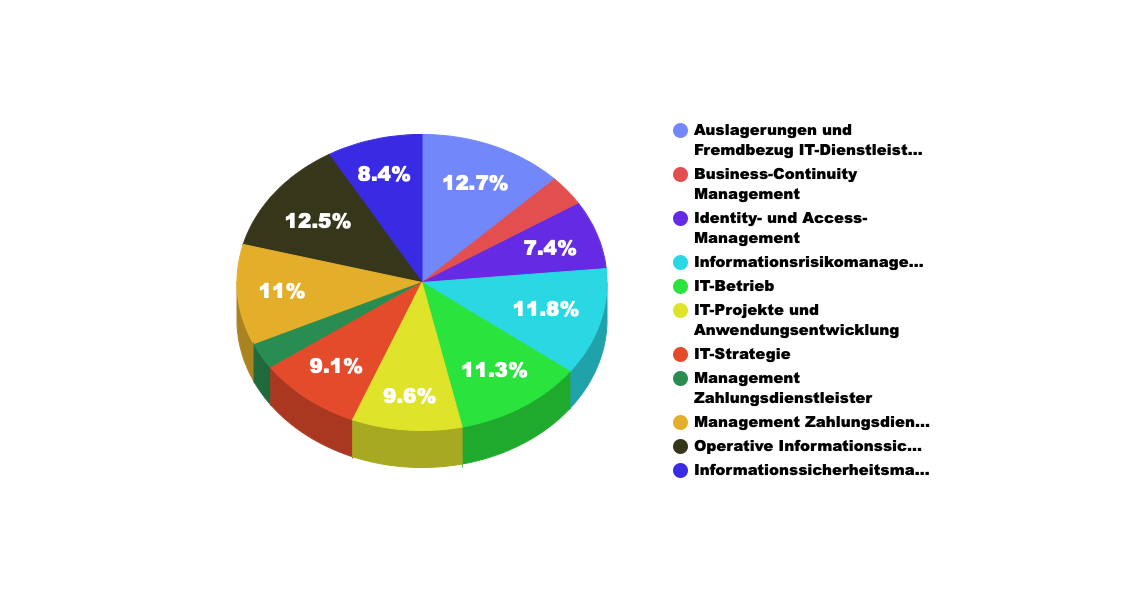
\includegraphics[width=\linewidth]{images/uploads/a_figure_02.png}
  \caption{Visuelle Darstellung der Aufteilung aller Anforderungen auf die definierten Kategorien. Quelle: Eigene Darstellung, 2022}
  \label{fig:kategorien_allg_aufteilung}
\end{figure}

%**********************************************************************************

\bigbreak
Betrachtet man in weiterer Folge nur jene Anforderungen die technisch umzusetzen sind, ergibt sich die in Tabelle \ref{table:kategorien_technisch} dargestellte Aufteilung. Es ist zu erkennen, dass die technisch umzusetzenden Anforderungen vorwiegend in den Kategorien \glqq{}Identity- und Access-Management\grqq{}, \glqq{}IT-Betrieb\grqq{} und vor allem in der Kategorie \glqq{}Operative Informationssicherheit\grqq{} zu finden sind. Abbildung \ref{fig:kategorien_technisch_aufteilung} zeigt die prozentuale Verteilung der technischen Anforderungen auf die unterschiedlichen Kategorien. 
\bigbreak
\begin{table}[H]
    \centering
    \caption{Zeigt die Kategorien der Anforderungsmatrix und die Anzahl der zugeordneten, technischen Anforderungen.} 
    \begin{tabular}{ll}
        \hline
        Kategorie & Anzahl\\
        \hline\hline
        Auslagerung und Fremdbezug IT-Dienstleistungen & 1\\
        Business-Continuity Management & 1\\
        Identity- und Access-Management & 30\\
        Informationsrisikomanagement & 7\\
        Informationssicherheitsmanagement & 11\\
        IT-Betrieb & 31\\
        IT-Projekte und Anwendungsentwicklung & 2\\
        IT-Strategie & 1\\
        Management Zahlungsdienstleister & 0\\
        Management Zahlungsdienstnutzer & 18\\
        Operative Informationssicherheit & 46\\
    \end{tabular}
    \label{table:kategorien_technisch}
\end{table}
\begin{figure}[H]
    \centering
  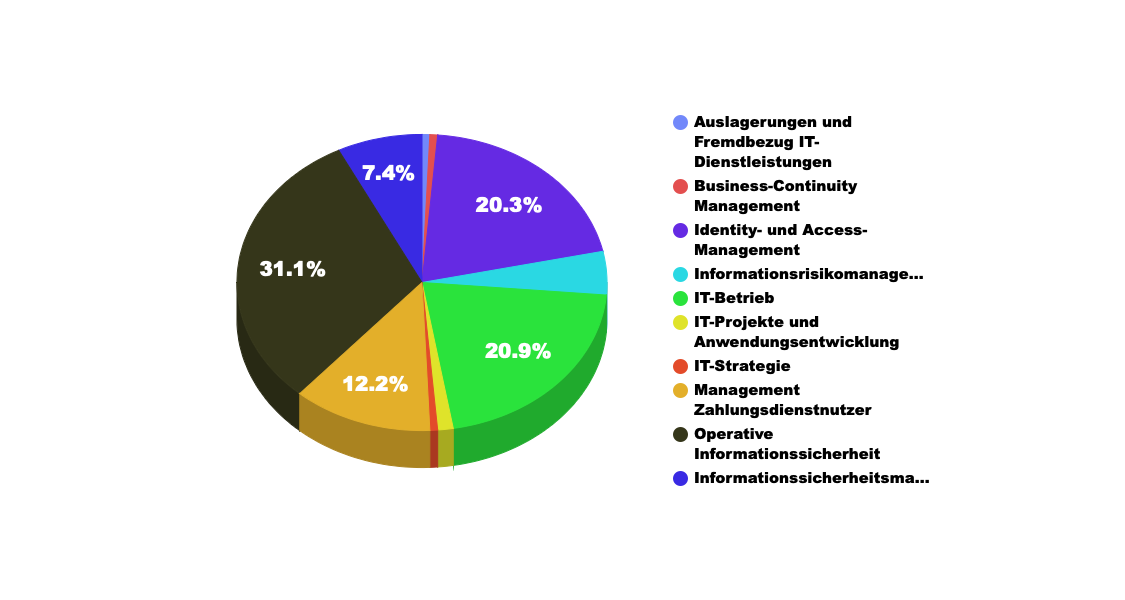
\includegraphics[width=\linewidth]{images/uploads/a_figure_04.png}
  \caption{Visuelle Darstellung der Aufteilung von technischen Anforderungen auf die definierten Kategorien. Quelle: Eigene Darstellung, 2022}
  \label{fig:kategorien_technisch_aufteilung}
\end{figure}
\bigbreak

Zur besseren Veranschaulichung wurden die organisatorisch und technisch umzusetzenden Anforderungen in Tabelle \ref{table:kategorien_vergleich_gesamt} direkt gegenübergestellt. Es ist zu erkennen, dass es nur eine Anforderungen aus dem Bereich \glqq{}Auslagerung und Fremdbezug IT-Dienstleistungen\grqq{} gibt, die sich technisch umsetzen lässt. Es handelt sich dabei um die Anforderung, dass Informationen die mit Drittanbietern ausgetauscht werden verschlüsselt übertragen werden müssen. Alle anderen Anforderungen liegen in der Durchführung bei dem jeweiligen Auslagerungspartner. Die technischen Anforderungen bestehen somit auf Seiten des Dritten. Auch im Bereich \glqq{}Business-Continuity Management\grqq{} besteht nur eine technische Anforderung. Es handelt sich dabei um die Notwendigkeit für eine redundante Auslegung von kritischen IT-Komponenten.
\bigbreak
Im Gegensatz zu den eben genannten Kategorien, sind 30 von 31 Anforderungen aus dem Bereich \glqq{}Identity- und Access-Management\grqq{} technischer Natur. Bei einer organisatorischen Anforderungen handelt es sich um die Notwendigkeit die implementierten, technischen Zugangskontrollen zu überwachen. Interessant ist, dass nur 5\% der Anforderungen aus dem Bereich \glqq{}IT-Projekte und Anwendungsentwicklung\grqq{} technisch erfüllt werden können. Es geht dabei um die Vorgabe, dass eigens erstellte Anwendungen auf mögliche Abweichungen vom Regelbetrieb zu überwachen und die Integrität der Anwendung, insbesondere des Quellcodes, angemessen sicherzustellen ist. 
\bigbreak
Ein weiterer Ausreißer findet sich im Bereich \glqq{}IT-Strategie\grqq{}. Nur eine Anforderung kann technisch umgesetzt werden. Es geht dabei um die Notwendigkeit, dass die Geschäftsleitung imstande sein muss Aussagen zu selbst entwickelten oder selbst betriebenen IT-Systemen treffen zu können. Auch wenn für die Umsetzung der Anforderung nur Informationen nötig sind, kann die Effizienz durch ein Verwaltungssystem, wie beispielsweise einer Content-Management-Database (CMDB) gesteigert werden. Im Bereich \glqq{}Operative Informationssicherheit\grqq{} bestehen 6 Anforderungen die organisatorisch umzusetzen sind. Diese Anforderungen wurden nicht als \glqq{}Technische Anforderung\grqq{} deklariert, da die Umsetzung vorrangig organisatorisch zu definieren ist. Ein Beispiel hierfür ist die Vorgabe, dass ein Zahlungsdienstkunde eine Warnung erhält, bevor eine dauerhafte Sperre seines Accounts in Kraft tritt.
\bigbreak

\begin{table}[H]
    \centering
    \tiny
    \caption{Zeigt alle Kategorien und die Anzahl der zugeordneten Anforderungen.} 
    \begin{tabular}{llll}
        \centering
        Kategorie & Gesamt & Organisatorisch & Technisch\\
        \hline\hline
        Auslagerung und Fremdbezug IT-Dienstleistungen & 53 & 52 & 1\\
        Business-Continuity Management & 14 & 13 & 1\\
        Identity- und Access-Management & 31 & 1 & 30\\
        Informationsrisikomanagement & 49 & 42 & 7\\
        Informationssicherheitsmanagement & 35 & 14 & 11\\
        IT-Betrieb & 47 & 16 & 31\\
        IT-Projekte und Anwendungsentwicklung & 40 & 38 & 2\\
        IT-Strategie & 38 & 37 & 1\\
        Management Zahlungsdienstleister & 12 & 12 & 0\\
        Management Zahlungsdienstnutzer & 46 & 28 & 18\\
        Operative Informationssicherheit & 52 & 6 & 46\\
    \end{tabular}
    \label{table:kategorien_vergleich_gesamt}
\end{table}
\bigbreak
%**********************************************************************************

Im Zuge der Auswertung der Anforderungsmatrix wurden auch die Risikofaktoren näher betrachtet. Abbildung \ref{fig:risiko_allg_aufteilung} zeigt die Verteilung der Risikofaktoren bezogen auf die abgeleiteten Anforderungen. Es ist zu erkennen, dass sich je ein Drittel der Risiken auf die beiden Bereiche \glqq{}Technisch\grqq{} und \glqq{}Organisatorisch\grqq{} verteilen. Daraus lässt sich ableiten, dass zwei Drittel der Anforderungen auf den Schutz der Infrastruktur und der internen Abläufe und Prozesse des Unternehmens ausgelegt sind. 
\begin{figure}[H]
    \centering
  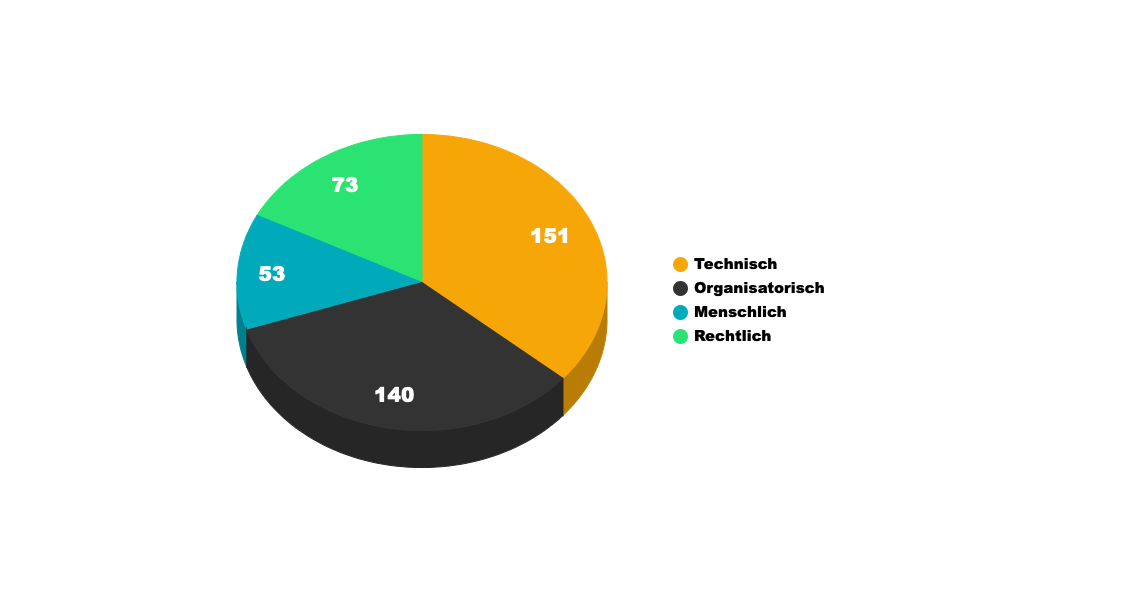
\includegraphics[width=\linewidth]{images/uploads/a_figure_03.png}
  \caption{Visuelle Darstellung der Aufteilung der Risikofaktoren aller Anforderungen. Quelle: Eigene Darstellung, 2022}
  \label{fig:risiko_allg_aufteilung}
\end{figure}
\bigbreak
Abbildung \ref{fig:risiko_technisch_aufteilung} zeigt die Verteilung der technischen Anforderungen auf die unterschiedlichen Risikofaktoren. 
Wie zu erwarten war, adressieren ein Großteil der Anforderungen den \glqq{}Technischen Risikofaktor\grqq{}. Interessant ist hierbei, dass 23 Anforderungen Bezug auf den \glqq{}Menschlichen Risikofaktor\grqq{} nehmen. Es handelt sich dabei um die Anforderungen aus dem Bereich \glqq{}Identity- und Access-Management\grqq{}. Betrachtet man die technischen Anforderungen die den \glqq{}Rechtlichen Risikofaktor\grqq{} adressieren, handelt es sich dabei um die Anforderungen zum Schutz von Transaktionsüberwachungen im Bereich Onlinebanking. Können betrügerische Zahlungen nicht erkannt oder etwa persönliche Sicherheitsmerkmale von Kunden nicht geschützt werden, kann dies rechtliche Konsequenzen für das Unternehmen mit sich ziehen. Bei den technischen Anforderungen die das \glqq{}Organisatorische Risiko\grqq{} adressieren, handelt es sich großteils um Anforderungen zum Umgang und der Verwaltung von IT-Ressourcen. Eine fehlende Verwaltung oder ein nicht definierter Umgang mit IT-Ressourcen kann zu Problemen beim Ablauf interner Prozesse führen und so die Stabilität des Unternehmens gefährden. Anforderungen mit \glqq{}Technischem Risikofaktor\grqq{} beziehen sich unter anderem auf die Implementierung von IT-Sicherheitsmaßnahmen und den Schutz von IT-Ressourcen und Daten. In Anbetracht der Tatsache, dass hierbei nur Anforderungen betrachtet wurden die technisch umgesetzt werden können, erscheint die Aufteilung legitim. 
\begin{figure}[H]
    \centering
  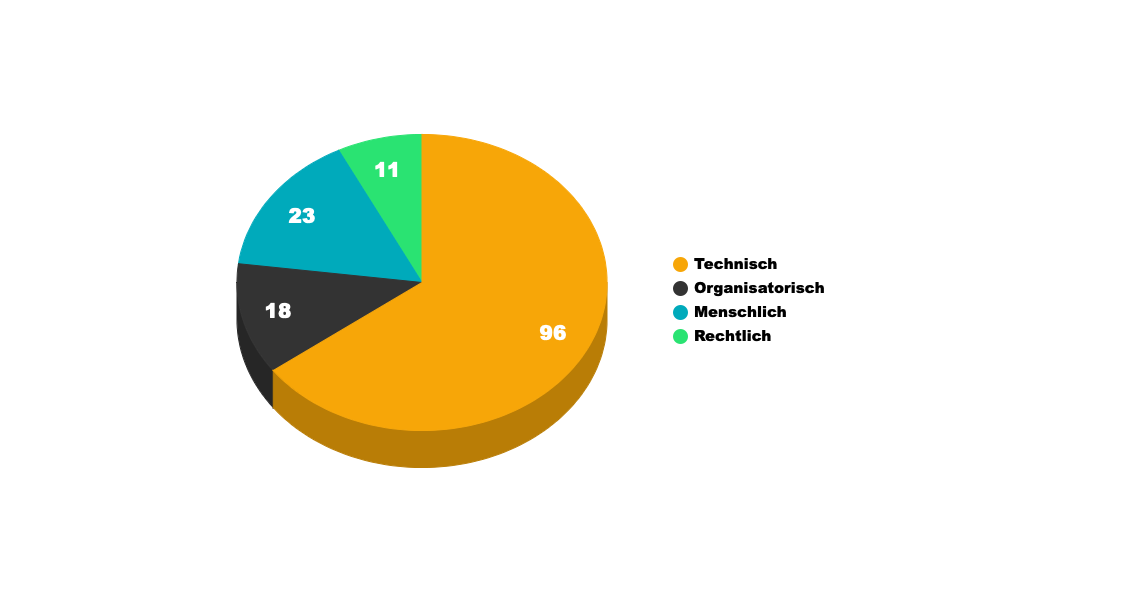
\includegraphics[width=\linewidth]{images/uploads/a_figure_05.png}
  \caption{Visuelle Darstellung der Aufteilung der Risikofaktoren technischer Anforderungen. Quelle: Eigene Darstellung, 2022}
  \label{fig:risiko_technisch_aufteilung}
\end{figure}

%**********************************************************************************
% Karacitel Abgeleitete Maßnahmen
%**********************************************************************************
\section{Abgeleitete Maßnahmen}
\label{kap_anforderungsmatrix_abgleitete_maßnahmen}
Dieses Kapitel gibt eine Übersicht über die aus den Anforderungen abgeleiteten Maßnahmen und zeigt, wie viele Anforderungen die einzelnen Maßnahmen abdecken. Auf Basis dieser Anforderungen wird in weiterer Folge versucht, Best-Practice-Ansätze für die Umsetzung der technischen IT-Sicherheitsvorgaben abzuleiten. Die nötigen Informationen für die Evaluierung der einzelnen Maßnahmen erfolgte auf Basis von Recherchen im Internet und Befragung von Mitarbeitern aus dem Bereichen \glqq{}IT-Security\grqq{} und \glqq{}IT-Infrastruktur\grqq{} einer Bank in Österreich.
\bigbreak
Im Zuge der Erstellung der Anforderungsmatrix wurde im Bereich \glqq{}Umsetzbarkeit\grqq{} definiert, ob die jeweilige Anforderung technisch oder organisatorisch umgesetzt werden kann. Der Bereich \glqq{}Beschreibung\grqq{} bietet eine Zusammenfassung für eine mögliche Umsetzung. Die Bereiche \glqq{}Abgedeckt durch Maßnahme x\grqq{} geben eine Übersicht über mögliche technische Maßnahmen, mit denen die Anforderung umgesetzt werden kann. Für die Evaluierung der möglichen Maßnahmen wurden pro Anforderung folgende Schritte durchgeführt:
\begin{enumerate}
    \item Recherche im Internet mit Hilfe der Informationen aus den Bereichen \glqq{}Kategorie\grqq{}, \glqq{}Titel der Anforderung\grqq{} und \glqq{}Definition\grqq{} der Anforderungsmatrix.
    \item Recherche von möglichen Hardware-/Softwareprodukten zur Adressierung der jeweiligen Anforderung.
    \item Befragung von Mitarbeitern aus den Bereichen \glqq{}IT-Infrastruktur\grqq{}, \glqq{}IT-Technik\grqq{} und \glqq{}Security-Operation-Center\grqq{} einer Bank in Österreich.
\end{enumerate}
\bigbreak
Tabelle \ref{table:maßnahmen_uebersicht_anzahl} zeigt eine Auflistung der abgeleiteten Maßnahmen und die Anzahl der technischen Anforderungen, die mit der jeweiligen Maßnahme umgesetzt werden können. Bei dieser Auswertung ist zu beachten, dass Anforderungen auch mit mehr als einer Maßnahme umgesetzt werden können. Aus diesem Grund variieren die Anzahl der technischen Anforderungen und die Anzahl der in Tabelle \ref{table:maßnahmen_uebersicht_anzahl} dargestellten Maßnahmen.
Interessant ist hierbei, dass sich 15\% der Anforderungen mittels der Adressierung von \glqq{}Identity-Management\grqq{} umsetzen lassen. Das bedeutet, dass Aufsichtsbehörden großen Wert auf den korrekten Umgang mit Berechtigungen und Accounts legen. 10\% der Anforderungen können durch die Betrachtung von \glqq{}Vulnerability-Management\grqq{} und weitere 9\% durch \glqq{}Security Incident und Event Monitoring\grqq{} adressiert werden. Daraus resultiert die Tatsache, dass sich ein Drittel der technischen Anforderungen für IT-Sicherheit an eine Bank in Österreich mit der Implementierung von drei Maßnahmen umsetzen lassen. 


\begin{table}[H]
    \centering
    \caption{Zeigt eine Übersicht über die analysierten Maßnahmen und die Anzahl der adressierten, technischen Anforderungen.} 
    \begin{tabular}{llll}
        Maßnahme & Anzahl adressierter Anforderungen\\
        \hline\hline
        Identity-Management & 32\\
        Vulnerability-Management & 21\\
        Security Incident und Event Monitoring & 20\\
        Kryptografie & 17\\
        Content-Management Database & 15\\
        Multifaktor-Authentifizierung & 15\\
        Patch-Management & 15\\
        Zentrales Log-Management & 13\\
        Netzwerksegmentierung & 11\\
        Monitoring & 10\\
        Single-Sign On & 10\\
        Backup and Restore & 10\\
        Endpoint-Detection and Response & 7\\
        Penetration-Testing & 6\\
        Baselining und Change-Management & 4\\
        Sourcecode Verwaltung & 4\\
        Native-Change Detection & 3\\
        Privileged-Access Management & 3\\
        Hochverfügbarkeit & 3\\
        Firewalls & 2\\
        Network-Access Control & 1
    \end{tabular}
    \label{table:maßnahmen_uebersicht_anzahl}
\end{table}
\setlength{\parindent}{0em} 

%**********************************************************************************
% Kapitel Best-Practice-Ansätze
%**********************************************************************************
\chapter{Best-Practice-Ansätze}
\label{cha:Auswertung}
In diesem Kapitel wird versucht, die in Kapitel \ref{kap_anforderungsmatrix_abgleitete_maßnahmen} abgleiteten technischen Maßnahmen in Bereiche zu Gruppieren. Auf Basis dieser Gruppen werden die einzelnen Maßnahmen beschrieben und Best-Practice-Ansätze definiert um eine umfassende und effiziente Adressierung der Maßnahmen zu ermöglichen. Die Gruppierung hat sich im Zuge der Ausarbeitung als sinnvoll ergeben, da unterschiedliche Maßnahmen ineinander greifen und voneinander profitieren.  
\bigbreak
Unter einem Best-Practice-Ansatz kann eine bestmögliche, bereits erprobte Methode oder Maßnahme zur Umsetzung einer Problemstellung verstanden werden. Ein Best-Practice-Ansatz stellt allerdings im allgemeinen Sprachgebrauch nur eine unverbindliche Empfehlung dar und unterscheidet sich somit von einem etablierten Standard. Die Empfehlung kann aufgrund Erfahrungen der jeweiligen Community entstehen oder sich im Laufe der Zeit als die effizienteste Methode etabliert haben. \autocite{duden} 
\bigbreak
Zur besseren Übersicht sind die Gruppen, die enthaltenen Maßnahmen und die abgeleiteten Best-Practice-Ansätze in Abbildung \ref{fig:bp-matrix} dargestellt. In weiterer Folge werden die einzelnen Gruppen und Best-Practice-Ansätze näher beschrieben
\begin{figure}[H]
    \centering
  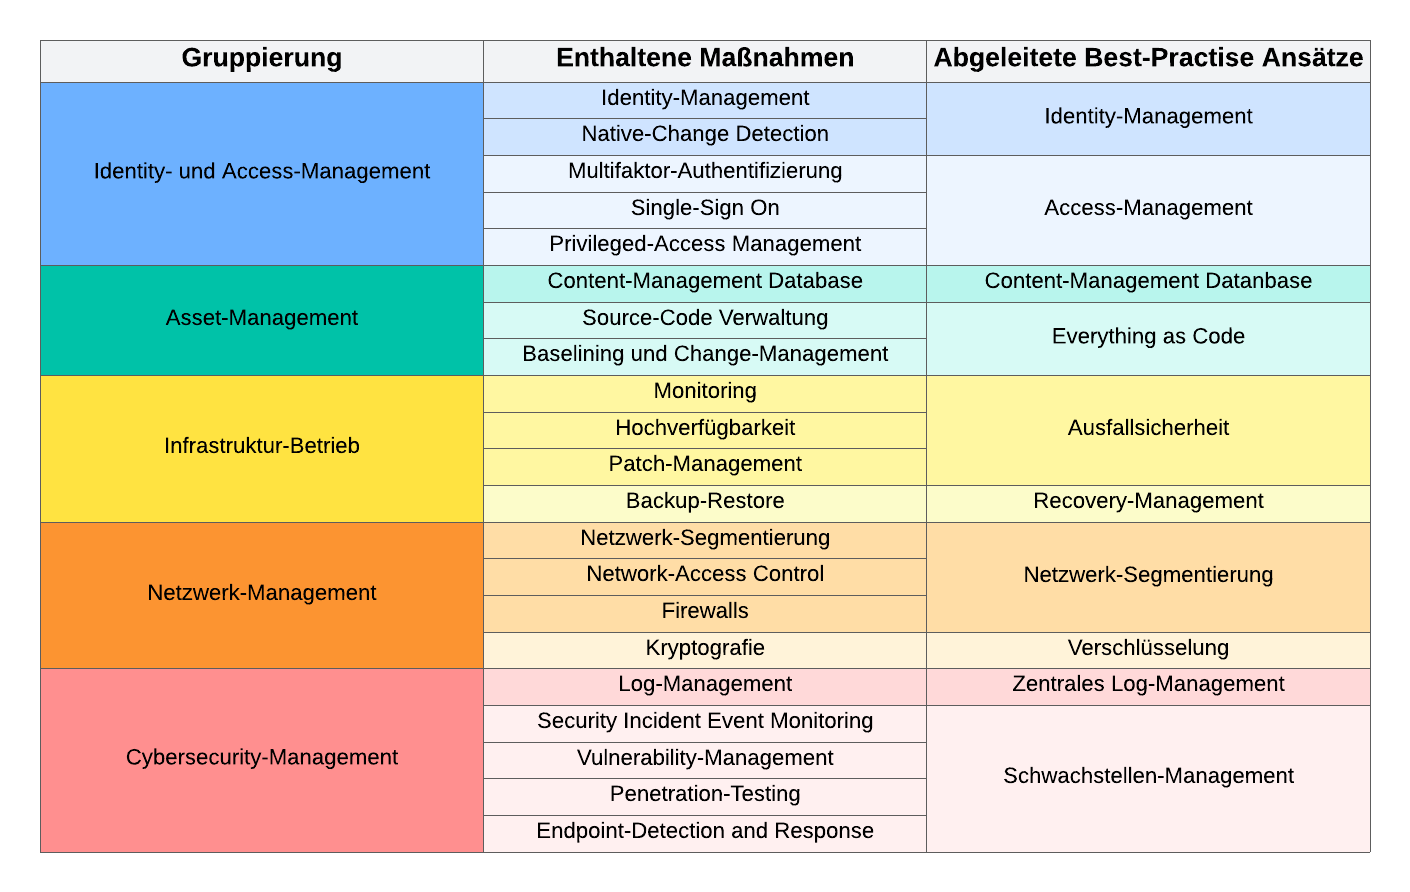
\includegraphics[width=\linewidth]{images/uploads/a_figure_15.png}
  \caption{Visuelle Darstellung der Gruppierungen, enthaltenen Maßnahmen und abgeleiteten Best-Practice-Ansätzen. Quelle: Eigene Darstellung, 2022}
  \label{fig:bp-matrix}
\end{figure}

\section{Identity- und Access-Management}
Die Gruppe \glqq{}Identity- und Access-Management\grqq{} (IAM) vereint die Maßnahmen \glqq{}Identity-Management\grqq{}, \glqq{}Privileged-Access Management\grqq{} (PAM), \glqq{}Multifaktor-Authentifizierung\grqq{} (MFA), \glqq{}Single-Sign On\grqq{} (SSO) und \glqq{}Native-Change Detection \grqq{} (NCD). Die Gruppe beschäftigt sich mit dem Lifecycle, der Authentifizierung und der Autorisierung von Identitäten und Benutzeraccounts.
\bigbreak
Darran Rolls und Morey J. Haber beschreiben in ihrem Buch \glqq{}Identity Attack Vectors: Implementing an Effective Identity and Access Management Solution\grqq{} fünf Grundpfeiler des IAM, die fünf \glqq{}A´s\grqq{} \autocite{rolls_haber_2020}:

\begin{itemize}
    \item Administration
    \item Audit
    \item Analyse
    \item Authentifizierung
    \item Autorisierung
\end{itemize}
\bigbreak
Die in der Gruppe IAM enthaltenen Maßnahmen decken jede für sich einen Teil der fünf A´s ab und tragen so zum Schutz von Identitäten und IT-Systemen bei. 

\subsubsection{Best-Practice-Ansatz: Identity-Management-System (IDM)}
Um Identitäten eines Unternehmens und deren zugeordnete Accounts in den unterschiedlichen Systemen verwalten zu können, ist eine globale Administration von beteiligten Identitäten erforderlich. Die in Kapitel \ref{kap_anforderungsmatrix_abgleitete_maßnahmen} abgleitete Maßnahme \glqq{}Identity-Management\grqq{} deckt die drei Bereiche \glqq{}Administration\grqq{}, \glqq{}Audit\grqq{} und \glqq{}Analyse\grqq{} ab. Eine globale Administration von Identitäten kann mit Hilfe eines \glqq{}Identity-Management Systems\grqq{} (IDM) realisiert werden. Ein IDM verwaltet Identitäten und bildet den gesamten Lifecycle einer Identität auf Basis von Prozessen ab. Zu diesem Lifecycle zählen das Erstellen der Identität, das Erstellen von Accounts, die Vergabe, Änderung und der Entzug von Berechtigungen. Das Ausscheiden einer Identität aus dem Unternehmen und damit einhergehend das Löschen aller zugehörigen Accounts schließt den Lifecycle ab. Ein IDM bietet somit die Möglichkeit den gesamten Lifecycle einer Identität zu definieren, durchzuführen und zu auditieren. Um dies zu ermöglichen werden unterschiedliche IT-Systeme, in Form von \glqq{}Applikationen\grqq{}, an das IDM angebunden. Beispiele für angebundene Applikationen sind etwa Benutzerdatenbanken auf die von unterschiedlichen anderen IT-Systemen zugegriffen wird. 
\bigbreak
Aufgrund der Tatsache, dass ein IDM System den gesamten Lifecycle von Identität und Berechtigungen abbildet, muss die Integrität der Daten gewährleistet werden. Aus diesem Grund wird ein IDM System als \glqq{}Single Source of Truth\grqq{} etabliert. Eine nicht autorisierte Änderung an einer Identität kann mittels NCD erkannt und behoben werden. Somit wird gewährleistet, dass ein IDM System bei einer direkten, nicht autorisierten Änderung in einem angebundenen System eingreifen kann. Eine mögliche Aktion des IDM wäre, dass die durchgeführte Änderung automatisch überschrieben und somit der vom IDM definierten Stand der Identität wieder herstellt wird. Mittels NCD können Unternehmen der Anforderung Nummer 317 laut Anforderungsmatrix nachkommen. In dieser Anforderung fordert die FMA, dass Unternehmen durch technisch-organisatorische Maßnahmen sicherzustellen haben, dass eine Manipulation der Berechtigungskonzepte verhindert wird.\\

Durch die Abbildung des Lifecycles von Identitäten und Berechtigungen innerhalb eines IDM wird auch weiteren Anforderungen von Aufsichtsbehörden nachgekommen. So ist laut Anforderung Nummer 315 aus der Anforderungsmatrix ein Unternehmen laut FMA verpflichtet, dass die Einräumung, Änderung, Deaktivierung und Löschung von Berechtigungen nachvollziehbar, zuordenbar und auswertbar dokumentiert wird. Diese Anforderung kann mit Hilfe eines IDM realisiert werden.
\bigbreak
Eine weitere Anforderung der FMA besteht darin, dass die den Identitäten eingeräumten Berechtigungen jederzeit, auditierbar sein müssen. Die Anforderung ist in der Anforderungsmatrix unter der Nummer 45 ersichtlich und kann mittels einer Rezertifizierung von Berechtigungen erfüllt werden. Im Zuge einer Rezertifizierung wird überprüft, welche Identitäten ein zu auditierendes Recht besitzen. Somit kann die Zuordnung einer bestimmten Berechtigung im Zuge einer Rezertifizierung legitimiert oder auch sämtlichen Identitäten gesammelt entzogen werden. Auch eine \glqq{}Separation of Duty\grqq{} (SoD) kann mittels eines IDM realisiert werden. Unter einer SoD versteht man eine Funktionstrennung von Identitäten. Mit Hilfe dieser Funktionstrennung soll beispielsweise vermieden werden, dass eine Identität die Berechtigung für das Anfordern eines Darlehens und gleichzeitig die Berechtigung für die Genehmigung dieses Darlehens besitzt. Das Vorhandensein von solchen Konstellationen kann mittels einer Analyse durch ein IDM überprüft werden.
\bigbreak
Ein Beispiel für ein IDM, das die beschriebenen Funktionen zur Verfügung stellt, ist \glqq{}Sailpoint Identity-IQ\grqq{} \autocite{Sailpoint_Identity_IQ}.

\subsubsection{Best-Practice-Ansatz: Access-Management}
Die beiden nach Darran Rolls und Morey J. Haber noch verbleibenden Grundpfeiler \glqq{}Authentifzierung\grqq{} und \glqq{}Autorisierung\grqq{} zählen zum Bereich des Access-Managements. 
\bigbreak
Unter einer Authentifizierung wird ein Login in Verbindung mit einer Art von Geheimnis, meist in der Ausprägung eines Passworts, verstanden. Eine Authentifizierung (v. griechischen \glqq{}authentikos\grqq{} für Urheber, der Echte, der Wirkliche), bezeichnet das Nachweisen einer Identität und den legitimen Zugang zu Privilegien, die der nachgewiesenen Identität zustehen. Alexander Tsolkas und Klaus Schmidt beschreiben in ihrer Arbeit \glqq{}Rollen und Berechtigungskonzepte - Identity- und Access-Management im Unternehmen\grqq{} die Möglichkeit zur Durchführung einer Authentifizierung mittels drei unterschiedlichen Objekten \autocite{TsolkasAlexander2010RuB:}: 

\begin{itemize}
    \item Preisgabe von Wissen (Passwort, PIN-Code, ...)
    \item Benutzung eines Besitzes (Token, ...)
    \item Benutzung des eigenen Subjekts (Retinascan, Fingerabdruck, ...)
\end{itemize}
\bigbreak
Die Authentifizierung einer Identität erfolgt im einfachsten Fall mittels Benutzername und Kennwort und wird von dem jeweiligen System durchgeführt, auf das die Identität zugreifen möchte. Das System nimmt hierfür den Benutzeraccount und das Passwort der Identität entgegen und verifiziert diese beiden Daten gegen eine Datenbank. Diese als \glqq{}Basic-Authentication\grqq{} bekannte Methode hat den Nachteil, dass jedes System für sich eine Abbildung der im IDM verwalteten Identitäten besitzen oder Zugriff auf die zugrunde liegende Datenbank haben muss. Mit der Anzahl der Systeme die Zugriff auf sensible Daten, wie etwa der Datenbank mit Benutzeraccounts und Kennwörtern benötigen, steigt auf das Risiko bei einer Kompromittierung des Systems. Gerade bei Systemen die beispielsweise aus dem freien Internet erreichbar sind oder nicht in der Verantwortung eines Unternehmens stehen, ist ein direkter Zugriff auf Benutzerdaten kritisch zu sehen. \autocite{rolls_haber_2020}
\bigbreak
Die EBA fordert in ihrer Leitlinie für das Management von IKT- und Sicherheitsrisiken, dass Authentifizierungsmethoden der Kritikalität der IKT-Systeme angemessen sein sollen. Diese Anforderung ist unter der Nummer 117 in der Anforderungsmatrix ersichtlich. Auf Basis dieser Anforderungen wurden Möglichkeiten etabliert, damit kritische Systeme nicht mit sensiblen Daten, wie etwa Passwörtern, in Berührung kommen. Eine Möglichkeit dafür bietet die Verwendung von Token-basierten Authentifizierungsmethoden, wie sie bei SSO-Systemen verwendet werden. Das \glqq{}OAuth 2.0 Protokoll\grqq{} beziehungsweise die Verwendung des Layers \glqq{}OpenID-Connect 1.0\grqq{} bietet Verfahren für diese Art der Authentifzierung. OAuth 2.0 ist ein offenes und standartisiertes Protokoll für die Token-basierte Authentifizierung im Internet \autocite{OAUTH2} \autocite{OpenID}. \\\\
Abbildung \ref{fig:token_auth} zeigt den Ablauf einer Authentifizierung mittels Token.  
Im Zuge der Authentifizierung sind drei Komponenten beteiligt. Der \glqq{}Browser\grqq{} symbolisiert die Identität, die Zugriff auf eine Ressource, die \glqq{}Applikation\grqq{} erhalten möchte. Der \glqq{}Authorization Server\grqq{} übernimmt die Rolle des SSO-Systems. Im ersten Schritt fordert der Browser Zugriff auf die Applikation. Innerhalb der Applikation wurde definiert, dass die Authentifizierung über den Authorization-Server stattfinden soll. Aus diesem Grund antwortet die Applikation mit einem Redirect zum Authorization-Server. Im Zuge des Redirects bietet der Authorization-Server eine Login-Seite, auf sich die Identität mittels Benutzername und Kennwort anmeldet. Der Authorization-Server validiert die von der Identität eingegeben Daten und antwortet mit einem Redirect zurück zur Applikation, gepaart mit einem zuvor generierten Authentication-Code. Im nächsten Schritt fordert die Applikation unter Verwendung des Authentication-Codes einen Token beim Authorization-Server an. Nach erfolgreicher Validierung des Authentication-Codes durch den Authorization-Server wird ein Token generiert und der Applikation übermittelt. Der Token stellt somit die Legitimation der Identität sicher. Aufgrund der Tatsache, dass die Applikation dem Authorization-Server vertraut, kann nun der Zugriff auf die Applikation gewährt werden. 
\bigbreak
Dieses Beispiel beschreibt die Möglichkeit einer Anmeldung an einem kritischen System. Der Vorteil liegt darin, dass das System selbst zu keinem Zeitpunkt der Anmeldung Kenntnis über die Logindaten der Identität erhält.

\begin{figure}[H]
    \centering
  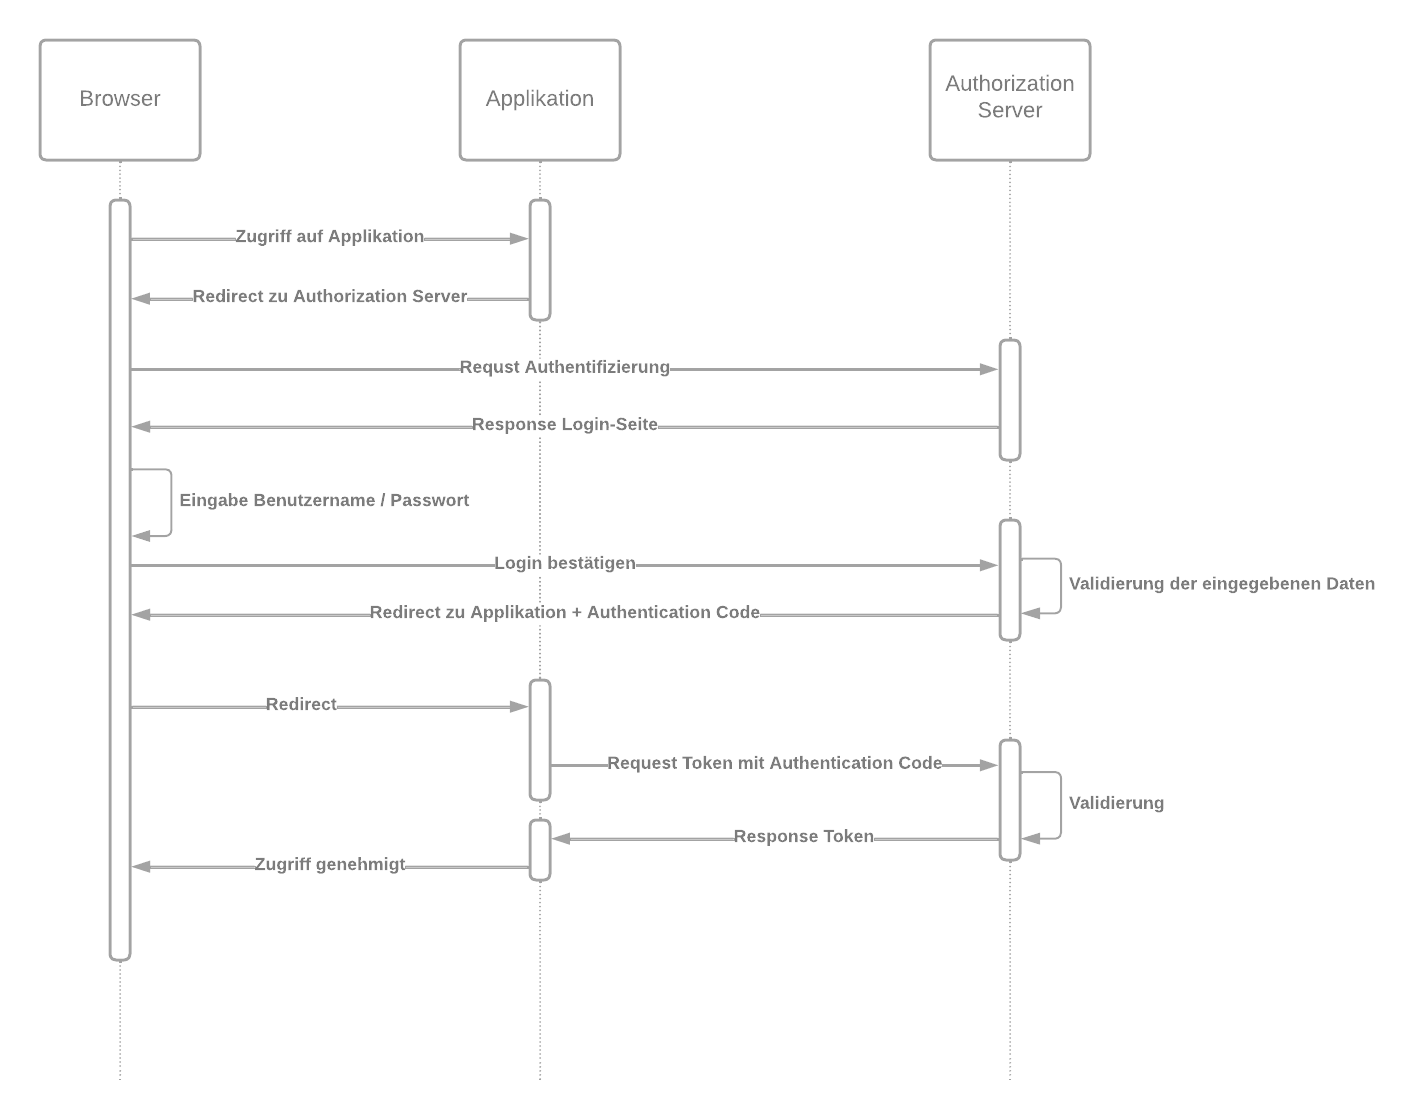
\includegraphics[width=\linewidth]{images/uploads/a_figure_06.png}
  \caption{Visuelle Darstellung einer Authentifizierung mittels Token. Quelle: Eigene Darstellung, 2022}
  \label{fig:token_auth}
\end{figure}

Die Authentifizierung über SSO kann hierbei noch um die Verwendung zusätzlicher Faktoren abgesichert werden. So benötigt eine Identität im Zuge der Authentifizierung neben dem Kennwort einen oder mehrere zusätzliche Faktoren, wie etwa einen zufällig generierten Code oder dem Vorhandensein einer Chip-Karte. MFA wird von vielen gängigen SSO-Frameworks, wie etwa \glqq{}Redhat Single Sign-On\grqq{} unterstützt \autocite{RedHat_SSO}. 
\bigbreak
Das Thema Access-Management bietet unterschiedliche Ausprägungen mit denen sich der Schutz von Identitäten und IT-Systemen verbessern lässt. PAM ist eine Subdisziplin im Bereich des IAM und eine Methode um privilegierte Aktivitäten auf Ressourcen abzusichern, zu kontrollieren, zu monitoren und zu managen. Unter einem privilegierten Account versteht man Accounts, die über besondere Berechtigungen verfügen. Beispiele hierfür sind lokale Administratoren, Service-Accounts, Domänen-Administratoren, privilegierte User-Accounts und C-Level Accounts. Das Ziel von PAM ist eine Risikominimierung, in dem privilegierter Zugriff auf Ressourcen nur dann gewährt wird, wenn die Notwendigkeit dafür besteht. Auf diese Weise wird vermieden, dass privilegierte Accounts während der täglichen Arbeit verwendet werden oder diese von Angreifern ausgenutzt werden können. Letzeres wird dadurch gewährleistet, dass Kennwörter für privilegierte Accounts erst bei Anforderung generiert werden. Abbildung \ref{fig:best-practice PAM} zeigt einen Möglichen Ablauf für den Zugriff auf eine Ressource durch einen Administrator unter der Verwendung von PAM. Es ist zu erkennen, dass der privilegierte Zugriff auf eine Ressource on-demand angefordert und von einem Dritten genehmigt werden muss. Der privilegierte Zugriff wird nach Beendigung des Tasks oder nach einem zuvor definierten Zeitraum automatisch entfernt. \autocite{rolls_haber_2020} 

\begin{figure}[H]
    \centering
  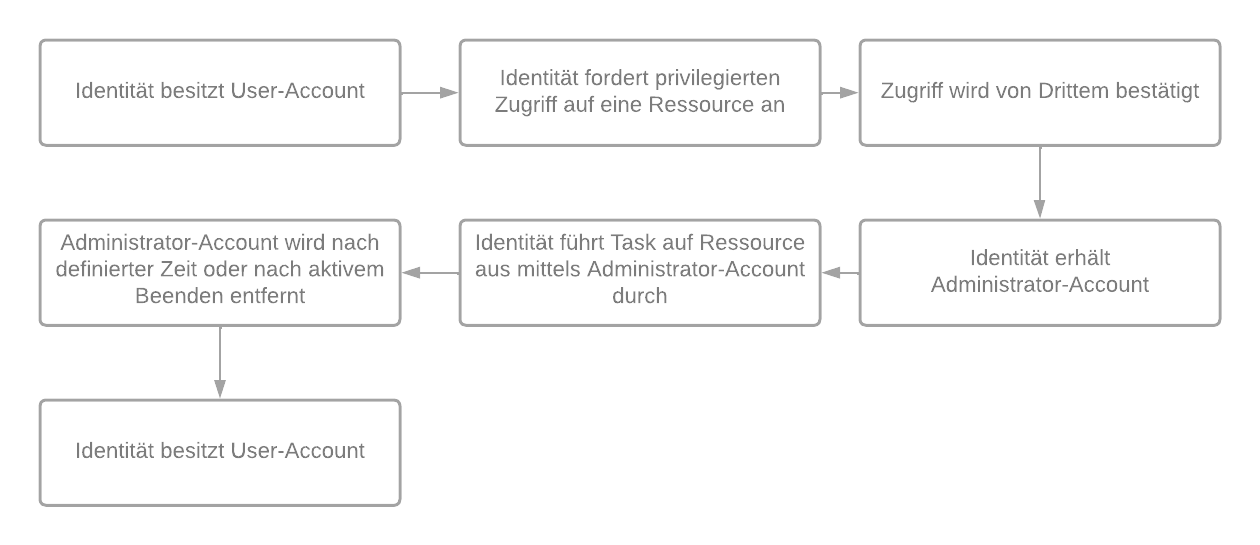
\includegraphics[width=\linewidth]{images/uploads/a_figure_07.png}
  \caption{Visuelle Darstellung des Zugriffs auf eine Ressource mittels PAM. Quelle: Eigene Darstellung, 2022}
  \label{fig:best-practice PAM}
\end{figure}

Mit Hilfe von PAM kann das \glqq{}Least-Privilege\grqq{} Modell, das Prinzip der minimalen Rechtevergabe realisiert werden. Dieses Prinzip wird sowohl von der EBA als auch von der BaFin gefordert. Die Anforderungen sind in der Anforderungsmatrix unter Nummer 41 und Nummer 111 hinterlegt. 
\bigbreak
Die beiden Best-Practice-Ansätze und die jeweiligen technischen Umsetzungen SSO, MFA, NCD und PAM adressieren die von Darran Rolls und Morey J. Haber beschriebenen Grundpfeiler der Authentifizierung und Autorisierung und decken die von Aufsichtsbehörden gesetzten Anforderungen aus dem Bereich IAM ab. 

\section{Asset-Management}
Die Gruppe \glqq{}Asset-Management\grqq{} vereint die Maßnahmen \glqq{}Content-Management\\-Database\grqq{}, \glqq{}Source-Code-Verwaltung\grqq{} und \glqq{}Baselining und Change-Management\grqq{}. Die Gruppe beschäftigt sich mit der Dokumentation, Sicherung, Änderung und Bereitstellung von Asset-Daten. 
\bigbreak
Eine zentrale und konsistente Übersicht über den aktuellen Zustand der gesamten IT-Umgebung ist ein wesentlicher Grundstein für einen reibungslosen Betrieb und die Implementierung und Sicherstellung der IT-Sicherheit im Unternehmen. Aus diesem Grund fordert die EBA, dass Unternehmen eine Übersicht über eigene IT-Assets und IKT-Systeme besitzen und diese Übersicht stets aktuell zu halten haben. Des Weiteren sind Unternehmen verpflichtet ein aktuelles Verzeichnis über die eigenen IKT-Assets zu führen und deren Verbindungen und Abhängigkeiten zueinander darzustellen. Diese beiden Anforderungen sind in der Anforderungsmatrix unter Nummer 97 und Nummer 136 ersichtlich. Die FMA fordert Abhängigkeiten von IT-Systeme abzubilden, das IT-Inventar zu verwalten und entsprechend zu steuern (Anforderungsmatrix Nummer 275). Die BaFin fordert, dass Unternehmen jederzeit einen aktuellen Überblick über die Bestandteile des festgelegten Informationsverbunds und deren Abhängigkeiten geben können. Außerdem muss die Geschäftsleitung imstande sein Aussagen zu selbst betriebenen IT-Systemen treffen zu können. Die Anforderungen der Bafin sind in der Anforderungsmatrix unter Nummer 5 und Nummer 7 ersichtlich. 

\subsubsection{Best-Practice-Ansatz: Configuration Management Database}
Eine \glqq{}Configuration Management Database\grqq{} (CMBD) ist eine Möglichkeit um den Anforderungen der Aufsichtsbehörden in diesem Bereich nachzukommen. Eine CMDB unterstützt Unternehmen dabei stets einen aktuellen Überblick über alle IT-Systeme, aktuelle Konfigurationen und betriebenen Services zu erhalten. Des Weiteren bildet eine CMDB die Grundlage für unterschiedliche IT-Sicherheitssysteme und nachgelagerte Automatisierungswerkzeuge, die auf Basis der von der CMDB bereit gestellten Daten arbeiten. Eine CMDB aggregiert  die Datenstände unterschiedlicher Systeme, korrelliert diese und wertet sie aus. 
\bigbreak
Für eine optimale Darstellung der IT-Landschaft ist die zugrund liegende Datenqualität von höchster Priorität. Die benötigten Konfigurationsdaten der einzelnen IT-Systeme manuell zu erheben gestaltet sich mit steigender Komplexität der IT-Infrastruktur unwirtschaftlich bis hin zu unmöglich. Für die Aggregation der Daten können automatische Discovery-Tools unterstützen. Ein Beispiel hierfür sind \glqq{}Endpoint-Detection and Response Systeme\grqq{} (EDR) wie Tanium\footnote{https://www.tanium.com}, die auf allen IT-Assets installiert werden. Mit Hilfe von Tanium können Echtzeitdaten der IT-Assets ausgelesen und an die CMDB übermittelt werden. Ein weiterer Vorteil von Tanium besteht darin, dass auch IT-Assets auf denen Tanium nicht installiert werden kann, erkannt werden können. Beispiele hierfür sind Netzwerk-Komponenten oder Appliance-Lösungen. Tanium erkennt und analysiert diese Systeme auf Basis der Verbindungen zu Systemen auf denen Tanium bereits installiert wurde. 
\bigbreak
Trotz der Verwendung von Tools wie Tanium können physikalische Komponenten in Unternehmen betrieben werden, nicht nicht automatisch erkannt werden können. Hier ist die Einbindung in Prozesse wie dem Change-Management relevant um einen stets aktuellen und konsistenten Datenstand zu erhalten. Eine CMDB kann neben der technischen Daten eines IT-Assets noch weitere Informationen enthalten. So kann die Beschreibung eines IT-Assets aus folgenden Komponenten bestehen:

\begin{itemize}
    \item Technische Daten
    \begin{itemize}
        \item IP-Adresse
        \item MAC-Adresse
        \item CPU, RAM, ...
    \end{itemize}
    \item Geografischer Standort
    \item Betriebssystem
    \begin{itemize}
        \item Version
        \item Lizenzkey
        \item Lizenzvertrag
    \end{itemize}
    \item Seriennummer
    \item Inventarnummer
    \item Servicevertrag
    \item SLA-Level
    \item Applikationen
    \item Sonstige Dokumente
\end{itemize}
\bigbreak
Anhand dieser Informationen lässt sich auf Basis unterschiedlicher Informationsquellen ein Gesamtbild der IT-Infrastruktur erstellen und den Anforderungen von Aufsichtsbehörden nachkommen.

\subsubsection{Best-Practice-Ansatz: Everything as Code (EaC)}
Auch in Bezug auf die Nachvollziehbarkeit von Änderungen an Assets werden Anforderungen gestellt. Die EBA und die BaFin fordern, dass Organisationen die Integrität der Anwendungen und Systeme angemessen sicherzustellen haben. Des Weiteren müssen Vorkehrungen getroffen werden um versehentliche Änderungen oder absichtliche Manipulationen erkennen zu können. Diese Anforderungen sind in der Anforderungsmatrix unter den Nummern 54 und 125 ersichtlich. Unternehmen sind laut BaFin weiters dazu verpflichtet, Änderungen an IT-Systemen in geordneter Art und Weise aufzunehmen, zu dokumentieren, zu bewerten, zu genehmigen und zu koordinieren (Anforderungsmatrix Nummer 63). Laut EBA sind Konfigurationsbaselinies für alle Netzwerkkomponenten zu implementieren.
\bigbreak
EaC ist eine Technik, in der sämtliche Teile eines Systems als Code behandelt werden. Dieses Prinzip wird bereits verstärkt im Bereich der Softwareentwicklung verwendet, wo sämtlicher Source-Code in Repositories wie etwa Apache-SVN\footnote{https://subversion.apache.org} oder Github\footnote{https://github.com} verwaltet wird, um eine SoT zu definieren. SoT beschreibt ein Konzept, in dem Daten von unterschiedlichen Systemen eines Unternehmens in einem bestimmten Platz aggregiert werden um Datensilos zu vermeiden. So wird sichergestellt, dass Systeme Daten von nur einer Quelle beziehen, welche stets den aktuellen Stand widerspiegelt. Ein \glqq{}Code-Repository\grqq{} (CR) ist der erste Schritt in der Deployment-Pipeline vom Source-Code hin zum fertigen Produkt oder System. Im Zuge des Deployment-Prozesses werden unterschiedliche Schritte, wie etwa automatische Tests oder automatische Freigabeprozesse in der Pipeline durchgeführt. Ein CR bildet somit einen Baustein für die von den Aufsichtsbehörden definierten Anforderungen. \autocite{mulesoft} \autocite{openpracticelibrary}
\bigbreak
Gerade mit der Etablierung der DevOps Bewegung, in der sich die Bereiche „Software- Development“ und „IT-Operations“ zusammenschließen, um einen sicheren, effizienteren und vor allem automatisierten System-Lifecycle zu definieren, nimmt die Vorgehensweise der Behandlung von Komponenten als Code, neben der Softwareentwicklung auch verstärkt Einzug in anderen Bereiche der IT. \autocite{könig_kugel_2019}
\bigbreak
Einer dieser Bereiche ist die IT-Infrastruktur, in der sich der Grad der Automation häufig auf wiederausführbare Skripte oder speziell angepasste Betriebssystem-Images begrenzt. Darüber hinausgehende Konfigurationen werden manuell oder mit Skripten, welche eigens für den jeweiligen Server angepasst werden, durchgeführt. \glqq{}Infrastructure as Code\grqq{} (IaC) übernimmt die Bereitstellung und die Konfiguration der gesamten Infrastruktur im Quellcode und ermöglicht das Schaffen von konsistenten und wiederholbaren Routinen. \autocite{özel_pautz_schmidt_2020}
\bigbreak
Unterschiedliche Anbieter von Container Virtualisierungslösungen, wie etwa Docker\footnote{https://www.docker.com} oder Redhat-Openshift\footnote{https://www.openshift.com}, arbeiten bereits mit einheitlichen Konfigurationen, welche Server oder Applikationen auf Basis von Templates beschreibend definieren, um diese so vom jeweiligen Framework plattformunabhängig provisionieren zu lassen. Weitere wichtige Themen, die eng mit dem Provisioning von Servern oder Applikationen verbunden sind werden häufig separat in anderen Tools behandelt oder gar nicht berücksichtigt. Zu diesen Themen zählen unter anderem das Erstellen von Dokumentationen, dem Berücksichtigen und Auditieren von Berechtigungsfreigaben oder dem Einpflegen und Berücksichtigen von IT- Sicherheitsrichtlinien.
\bigbreak
Einen weiteren Bereich, der von der Behandlung von Komponenten als Code profitieren kann, bildet der Compliance-Bereich, die Einhaltung von Governance-Richtlinien. Mit Hilfe von \glqq{}Policy as Code\grqq{} (PaC) wird versucht bei der Überprüfung auf Richtlinien weg von einem manuellen Ansatz der von Menschen durchgeführt wird, hin zu einem konsistenten, effizienten und wiederholbaren Ansatz der Überprüfung von Richtlinien, auf Basis von Code zu kommen. \autocite{hashicorp_policyascode}
\bigbreak
Der Zusatz \glqq{}as Code\grqq{} weist auf die der jeweiligen Technologie hinzugefügten Attribute Effizienz, Sicherheit, Transparenz und Automatisierung hin und versucht diese Themen ebenso im Zuge des Provisionings zu berücksichtigen. Spricht man von \glqq{}codification\grqq{} bedeutet dies den Erhalt von automatisierten Tests, einer einheitlichen Sprache, welche sowohl von IT-affinen als auch Mitarbeiter aus dem organisatorischem Umfeld verstanden werden kann, und einer automatisierter Deployment-Pipeline, welche sich modular um diverse Komponenten erweitern lässt. Eine Deployment-Pipeline beschreibt den automatisierten Prozess von der Erstellung des Quellcodes bis hin zum Provisioning des fertigen Produkts. Mit Hilfe unterschiedlicher Schritte ermöglicht eine Deployment-Pipeline die automatisierte Ausführung von Arbeitsschritten. Zu diesen Arbeitsschritten zählen unter anderem eine Versionierung des Quellcodes, eine automatisierte Freigabe von Änderungen, die Ausführung von Tests, das Deployment in eine Test-Umgebung und das anschließenden Deployment in die produktive Umgebung. \autocite{könig_kugel_2019}
\bigbreak
Auf Basis der Vorteile der Definition von Komponenten als Code, gliedert sich der Bereich EaC unter anderem in folgende Teilbereiche:
\begin{itemize}
    \item Infrastructure as Code
    \item Security as Code
    \item Policy as Code
\end{itemize}
\bigbreak
\textbf{Infrastructure as Code}\\
Mit Hilfe von IaC können die Anforderungen der BaFin und der EBA in Bezug auf Änderungen an Assets unter Einbezug eines Genehmigungsprozesses und der Etablierung von Konfigurationsbaselines nachgekommen werden. 
IaC versucht die Vorteile von EaC bezogen auf Infrastrukturkomponenten zu behandeln und abzudecken. Sämtliche Teile eines Systems, wie etwa die Konfiguration der virtuellen Umgebung, die Konfiguration des Betriebssystems, Einstellungen betreffend installierter Programme oder auch die Dokumentation dieser, werden in Repositories gespeichert.
Dies bringt unter anderem folgende Vorteile mit sich \autocite{hackernoon_2020}:
\begin{itemize}
    \item Nachvollziehbarkeit\\
        Änderungen an Systemen können jederzeit detailliert nachvollzogen oder rückgängig gemacht werden. Backups und Restores von Infrastrukturkomponenten sind großteils überflüssig, da die Komponenten ad-hoc neu provisioniert werden können.
    \item Wiederholbarkeit\\
        Systeme können jederzeit auf unterschiedliche Plattformen provisioniert werden (Ready for Cloud). Somit bietet IaC die Möglichkeit einer \glqq{}On Demand Infrastruktur\grqq{}.
    \item Testing\\
        Durch ein Testing Verfahren können Änderungen am System getestet und bei erfolgreichem Test automatisiert in der Produktionsumgebung provisioniert werden.
    \item Schutz vor Server- und Configuration Drift\\
        Es existiert nur mehr eine SoT. Änderungen, welche direkt am Zielsystem vorgenommen und somit nicht in der SoT aufzufinden sind, werden automatisch überschrieben. Dies dient zum einen dem Erkennen von unautorisierten Änderungen von Einstellungen am System, zum anderen beugt es Configuration-Drifts vor. Darunter versteht man das Abweichen einer Konfiguration von einem definierten und gewünschten Zustand. Configuration-Drifts können etwa entstehen, wenn unterschiedliche Server von verschiedenen Mitarbeitern erstellt und konfiguriert werden. Obwohl alle Mitarbeiter nach denselben Vorgaben arbeiten, können sich Unterschiede in der Konfiguration ergeben. \autocite{morris}
    \item Dokumentation und Geteiltes Wissen\\
        Sämtliche Komponenten eines Systems werden an einer gesammelten Stelle dokumentiert und sind dort einsehbar. Arbeiten mehrere Personen, oder sogar unterschiedliche Teams, an ein und demselben System, kann das Wissen durch eine einheitliche Definitionssprache leichter vermittelt und die verwalteten Systeme schneller erfasst werden. Auch personellen Ausfällen kann so vorgebeugt werden. Bei Standalone-Lösungen kann es Mitarbeitern ohne einer vorhandenen Dokumentation Probleme bereiten, die ursprüngliche Intention des Erstellers oder manuelle Änderungen an einem System nachzuvollziehen.
    \item Freigabe und Audit\\
        Änderungen am System, ohne vorheriger Freigabe durch das Management, werden technisch unterbunden. Durch die zentrale Speicherung sämtlicher Komponenten eines Systems, werden etwaige Audit-Anfragen und Feedback-Schleifen signifikant beschleunigt.
\end{itemize} 
\bigbreak
Der Vollständigkeit halber wird auch noch auf die beiden anderen Teilbereiche von EaC eingegangen. Obwohl die Anwendungsgebiete von \glqq{}Security as Code\grqq{} (SaC) und \glqq{}Policy as Code\grqq{} (Pac) nicht explizit von den Aufsichtsbehörden gefordert sind, tragen sie dennoch stark zu einer sicheren und stabilen IT-Infrastruktur bei. 
\bigbreak
\textbf{Security as Code}\\
SaC beschreibt Techniken um Sicherheit bei der Entwicklung mittels einer Deployment-Pipeline zu gewährleisten. Im Zuge des jeweiligen Deployment-Prozesses werden automatisiert Sicherheitsüberprüfungen durchgeführt und nach Schwachstellen gesucht.
Folgende Überprüfungen können als Teil einer zusätzlichen Sicherheitsschicht integriert werden \autocite{hackernoon_2020}:
\begin{itemize}
    \item Automatische Vulnerarbility Scans
    \item Ausführung von Skript-Tests
    \item Überprüfung auf Default-Konfigurationen
    \item Implementierung von Monitoring Funktionalitäten
\end{itemize}
\bigbreak
Diese Ansätze bringen unter anderem folgende Vorteile mit sich \autocite{hackernoon_2020}:
\begin{itemize}
    \item Schnellere Reaktion auf Änderungen und Sicherheitsanforderungen
    \item Bessere Zusammenarbeit zwischen den einzelnen Teams
    \item Vulnerabilities können in einem frühen Stadium erkannt und behoben werden
    \item Entwicklungskosten können durch das automatisierte und frühzeitige Erkennen von
    Schwachstellen und Fehlern verringert werden
    \item Die Möglichkeit für automatisierte Sicherheitsüberprüfungen wird geschaffen
\end{itemize}
\bigbreak
\textbf{Policy as Code}\\
PaC beschreibt die Möglichkeit Richtlinien in einem Weg zu definieren, dass diese sowohl von Mensch als auch Maschine gelesen, interpretiert und validiert werden können.
Das Ziel von PaC ist es organisatorische Richtlinien des Unternehmens automatisch zu implementieren, verifizieren, monitoren und zu reporten. Ein großer Vorteil besteht darin, dass Richtlinien bereits im Zuge des Deployment-Prozesses behandelt werden können. So wird gewährleistet, dass bereits während der Entwicklung frühzeitig und nachvollziehbar auf potentielle Policy-Verletzung reagiert werden kann.

Um PaC zu ermöglichen können die jeweiligen Richtlinien codetechnisch abgebildet und in Form von Tests in den Deployment-Prozess integriert werden. Ein weiterer Weg ist, Richtlinien mit der Konfiguration der Deployment-Pipeline durchzusetzen. Auf diesem Weg können etwa unterschiedliche Aktionen oder Abläufe unterbunden werden. PaC baut somit automatisierte Compliance sowohl in der Entwicklung als auch im Betrieb auf.
Der Begriff „Policy“ ist in der Literatur nicht klar definiert und umfasst mehrere Bereiche \autocite{dadgar}:
\begin{itemize}
    \item Compliance Policies\\
    Diese Richtlinien schaffen Compliance unter Einbezug externer Standards wie
    dem „Payment Card Industry Security Standard“ (PCI-DSS5) oder der „General Data Protection Regulation“ (GDPR6) \autocite{PCIDSS5} \autocite{GDPR}.
    \item Security Policies\\
    Diese Richtlinien definieren interne Datenschutz- und Datensicherheits-Vorgaben eines Unternehmens um die Sicherheit und die Integrität von Daten zu schützen. Die Definition von Applikationen, welche vom freien Internet aus erreichbar sind, stellen ein Beispiel für eine Security Policy.
    \item Operational Excellence\\
    Diese Art von Policy verhindert Service-Ausfälle oder Service-Verschlechterungen zu Lasten des Unternehmens oder des Kunden. Beispiele hierfür sind die Validierung von neuen Konfigurationseinstellungen oder die Sicherstellung einer redundant ausgelegten Anbindung von Systemen.
\end{itemize}
\bigbreak
Die Definition von Richtlinien mittels PaC bietet unter anderem folgende Vorteile \autocite{hackernoon_2020}:
\begin{itemize}
    \item Routineberichte optimieren die Auditierung von Systemen\\
    Berichte, die während des gesamten DevOps-Lebenszyklus generiert werden liefern Dokumentation und Nachweis, mit deren Hilfe viele internen und behördlichen Prüfungsverfahren nachverfolgt und rationalisiert werden können.
    \item Compliance Transparenz
    \item Zeitersparnis
    \item Kontinuierliche Auditierbarkeit
\end{itemize}

\section{Infrastruktur-Betrieb}
\label{Patch-Management}
Die Gruppe \glqq{}Infrastruktur-Betrieb\grqq{} vereint die Maßnahmen \glqq{}Monitoring\grqq{}, \glqq{}Hochverfügbarkeit\grqq{}, \glqq{}Backup-Restore\grqq{} und \glqq{}Patch-Management\grqq{}. Die Gruppe beschäftigt sich mit der Aufrechterhaltung und der Absicherung von IT-Systemen um einen sicheren und stabilen Betrieb zu gewährleisten. 
Aufsichtsbehörden stellen unterschiedliche Anforderungen an den Betrieb und die Verfügbarkeit von IT-Systemen von Banken. Die BaFin fordert, dass Konzepte zur Hochverfügbarkeit implementiert, angewendet und entsprechend überprüft werden (Anforderungsmatrix Nummer 82). Die EBA fordert, dass Unternehmen Leistungs- und Kapazitätsplanungs- und -überwachungsprozesse einführen um bedeutende Leistungsprobleme von IKT-Systemen und Engpässe bei IKT-Kapazitäten rechtzeitg zu erkennen und darauf reagieren zu können (Anforderungsmatrix Nummer 139). Die FMA setzt weiters voraus, dass die Kontinuität und Ausfallsicherheit der IT-Systeme laufend überprüft und eine rechtzeitige Wiederherstellung von IT-Systemen nach Betriebsausfällen gewährleistet wird (Anforderungsmatrix Nummer 340). Außerdem werden Anforderungen an Update-Prozesse von Systemen gestellt. Die BaFin setzt voraus, dass Unternehmen IT-Systeme regelmäßig aktualisieren und die Stabilität der Systeme im Falle einer Änderung entsprechend testen (Anforderungsmatrix Nummer 61). Im Falle eines Ausfalls oder eines Datenverlusts setzt die EBA voraus, dass Unternehmen Verfahren zur Sicherung und Wiederherstellung von Daten und IKT-Systemen festlegen und umsetzen, um sicherzustellen, dass diese bei Bedarf wiederhergestellt werden können (Anforderungsmatrix Nummer 140). 
\bigbreak
Betrachtet man die Anforderungen der Aufsichtsbehörden, ergeben sich zwei Bereiche die von Banken in Österreich addressiert werden müssen \autocite{kharod_2021}:
\begin{itemize}
    \item Gewährleistung des stabilen Betriebs der IT-Infrastruktur (Ausfallsicherheit)
    \begin{itemize}
        \item Hochverfügbarkeit
        \item Monitoring
        \item Patch-Management
    \end{itemize}
    \item Reaktion auf Ereignisse betreffend IT-Infrastrukturkomponenten (Recovery Management)
    \begin{itemize}
        \item Backup-Restore
    \end{itemize}
\end{itemize}

\subsubsection{Best-Practice-Ansatz: Ausfallsicherheit}
Ist ein System \glqq{}hochverfügbar\grqq{} bedeutet das, dass das System lange Zeit ohne Unterbrechung stabil läuft. Die Verfügbarkeit eines Systems wird in Prozent gemessen. Besitzt ein System eine Verfügbarkeit von 100\%, ist keine Downtime zu erwarten. In der Realität kann eine Verfügbarkeit von 100\% nahezu ausgeschlossen werden. 
\bigbreak
Eine hochverfügbare Infrastruktur charakterisiert sich unter anderem durch folgende Eigenschaften:
\begin{itemize}
    \item Vermeidung von Single Points of Failure (SPoF)
    \item Redundanz / Load-Balancing
    \item Auto-Skalierbarkeit
    \item Monitoring
\end{itemize}
\bigbreak
SPoFs können in unterschiedlicher Ausprägung bestehen und stellen ein Bottleneck in der Ausfallsicherheit dar. Egal ob es sich bei der Instanz um einen einzelnen Server oder um ein ganzes Rechenzentrum handelt, fällt ein SPoF aus, hat dies Auswirkungen auf alle angebundenen IT-Systeme. 
\bigbreak
Hardware Redundanz wird erzielt in dem zwei oder mehr Instanzen einer Hardware Komponente bereitgestellt werden. Wird zusätzlich ein Load-Balancer implementiert, kann dieser die Last gleichmäßig auf die redundanten Hardware Komponenten verteilen, Lastspitzen abgefangen und die Systemstabilität gewährleisten. Eine weitere Möglichkeit um Lastspitzen abzufangen und auf steigende Auslastung zu reagieren ist die Skalierung von Systemen. Unter einer Auto-Skalierbarkeit versteht man die Fähigkeit von Systemen sich wachsenden oder schrumpfendnen Anforderungen hinsichtlich der Leistungsfähigkeit automatisch anzupassen. Es wird zwischen der vertikalen Skalierung (scale up) und der horizontalen Skalierung (scale out) unterschieden. Bei der vertikalen Skalierung wird Leistung innerhalb des IT-Systems hinzugefügt oder entfernt. Die Leistungssteigerung entsteht somit durch das Hinzufügen zusätzlicher Komponenten wie etwa Speicherplatz, CPUs oder zusätzlicher Grafikkarten. Bei der horizontalen Skalierung wird die Leistungssteigerung eines IT-Systems durch das Hinzufügen zusätzlicher Systeme erbracht. Die vom IT-System durchzuführenden Arbeiten wird auf unterschiedlichen Instanzen verteilt. So kann gewährleistet werden, dass steigender Workload mit gleichbleibender Performance abgearbeitet werden kann. \autocite{geißler_2019}
\bigbreak
Um die Stabilität von IT-Systemen gewährleisten und auf etwaige Störungen oder Lastspitzen entsprechend reagieren zu können, ist eine Überwachung der IT-Infrastruktur unumgänglich. \\
Bevor eine Überwachung implementiert wird, sollten folgende Punkte geklärt sein \autocite{ashutosh_nivedita_2022}:
\begin{itemize}
    \item Grund für das Monitoring\\
    Je nach Anwendungsfall kommen unterschiedliche Lösungen für ein Logging und ein Monitoring in Frage. Mögliche Gründe für ein Monitoring sind Compliance-Anforderungen, Gesetzliche Anforderungen oder Incident-Response-Anforderungen. 
    \item Daten, die für das Monitoring benötigt werden\\
    Für das Monitoring von Finanztransaktionen sind beispielsweise andere Daten sinnvoll und nötig, als für das Monitoring von Netzwerk-Komponenten. Unabhängig vom Anwendungsfall sollten Logeinträge folgende Informationen enthalten:
    \begin{itemize}
        \item Durchführender (Wer: Accountname oder IP-Adresse)
        \item Aktion (Was: Lesen/schreiben auf welcher Ressource)
        \item Zeitpunkt (Wann: Timestamp)
        \item Lokation (Wo: Geolocation, Browser, Skript-Name, ...)
    \end{itemize}
    \item Zu überwachende Assets\\
    Um zu verhindern, dass Logdaten die für das Monitoring nötig sind zu viel Speicherplatz in Anspruch nehmen, sollte im Vorfeld geklärt werden welche Assets zu überwachen sind. Basierend auf den jeweiligen Assets ist zu definieren, welche Software-Komponente überwacht werden soll und welcher Daten-Klassifizierung die gesammelten Daten entsprechen.
    \item Sicherheitsaspekt betrachten\\
    Basierend auf der Daten-Klassifizierung sind entsprechende Sicherheitsvorkehrungen zu treffen. Personenbezogene Daten sollten maskiert oder anonymisiert werden. Die Übertragung von Log-Daten sollte verschlüsselt stattfinden und der Zugriff auf den Zustand eines Systems oder einer Applikation einem rollenbasierten Berechtigungskonzept unterliegen.
    \item Automatisierung und Standardisierung\\
    Soweit möglich sollte ein Monitoring automatisiert stattfinden und das System im Fehlerfall automatisch die zuständige Person benachrichtigen. Um Monitoring-Alarme weiterverarbeiten zu können, sollten diese in einem standardisierten Format, etwa im Format \glqq{}JSON\grqq{} übergeben werden \autocite{JSON}.  
\end{itemize}

\bigbreak
Dies Überwachung von IT-Systemen kann mit unterschiedlichen Software-Produkten umgesetzt werden. Die Implementierung einer Monitoring-Software gestaltet sich vergleichsweise einfach. Eine viel größere Herausforderung bietet die Frage, welche Daten im speziellen betrachtet werden müssen um die Instabilität oder Auslastung von IT-Systemen zu erkennen. Um den Gesundheitsstatus eines Systems zu messen werden unterschiedliche Metriken definiert und auf den Systemen gemessen. Unter einer Metrik wird ein Datensatz verstanden, der die Performance und Verfügbarkeit von Ressourcen wiederspiegelt. Mit Hilfe von Metriken kann der Status eines Systems zu einer bestimmten Zeit gemessen und entsprechend interpretiert werden. \autocite{geißler_2019} 
\bigbreak
Datadog\footnote{https://www.datadoghq.com}, ein Betreiber von Software-as-a-Service Monitoring Diensten teilt Metriken in die zwei Kategorien \glqq{}Work-Metrics\grqq{} (WM) und \glqq{}Ressource-Metrics\grqq{} (RM). WM geben den Top-Level Status eines IT-Systems an, in dem die Leistung des Systems, bezogen auf die durchzuführende Tätigkeit gemessen wird. 
\bigbreak
WM lassen sich in vier Typen einteilen \autocite{le-quoc_2015}:
\begin{itemize}
    \item Throughput\\
    Gibt die Menge an Tasks an, die das System pro Zeiteinheit absolviert.
    \item Success\\
    Repräsentiert die Anzahl erfolgreich durchgeführter Tasks in Prozent.
    \item Error\\
    Repräsentiert die Anzahl an Fehlern, die ein System während der Durchführung von Tasks produziert.
    \item Performance\\
    Gibt die Effizienz des Systems im Zuge der Durchführung von Tasks an. 
\end{itemize}
\bigbreak
WM können dabei unterstützen eine generelle Aussage zum Status und der Performanz eines Systems zu treffen. So können WM beispielsweise Antwort auf folgende Fragen liefern:
\begin{itemize}
    \item Ist das System aktiv?
    \item Wie gut performed das System?
    \item Wie ist die Qualität der durchgeführten Tasks?
\end{itemize}
\bigbreak
Tabelle \ref{table:WM-Beispiele} zeigt ein Beispiel für mögliche WM eines Webservers bezogen auf die Anzahl von Requests und die Qualität der Reponses.\\ So werden im Schnitt 32 Requests pro Sekunde mit einer durchschnittlichen Antwort-Zeit von 0.4 Sekunden vom Webserver abgearbeitet. 99.1\% der Requests sind erfolgreich, 0.1\% der Requests bewirken einen Fehler vom Typ 5xx auf Serverseite. 
\bigbreak
\begin{table}[H]
    \centering
    \caption{Beispiel für Work-Metrics: Webserver, Quelle \autocite{le-quoc_2015}, 2022} 
    \tiny
        \begin{tabular}{lll}
            \hline
            Type & Beschreibung & Wert\\
            \hline\hline
            Throughput & Requests pro Sekunde & 32\\
            Success & Prozentualer Anteil von Web-Responses vom Typ 2xx seit der letzten Messung & 99.1\\
            Error & Prozentualer Anteil von Web-Responses vom Typ 5xx seit der letzten Messung & 0.1\\
            Performance & Durchschnittliche Response-Zeit in Sekunden & 0.4\\
        \end{tabular}
        \label{table:WM-Beispiele}
\end{table}
\bigbreak
Im Gegensatz zu WM liefern RM keine Auskunft über den Status der durchgeführten Tasks, sondern über den Status des überwachten Systems selbst. Am Beispiel des genannten Webservers sind etwa Ressourcen wie die Auslastung der CPU, des Arbeitsspeichers, der Festplatte und des Netzwerk-Interfaces relevant um den Status des Systems zu beschreiben.
\bigbreak
Für jede zu überwachende Ressource des Systems sind folgende vier Werte relevant \autocite{le-quoc_2015}:
\begin{itemize}
    \item Utilization\\
    Repräsentiert die anteilsmäßige Auslastung der Ressource in Prozent.
    \item Saturation\\
    Gibt die Anzahl an anstehenden Tasks an, die zum Messzeitpunkt noch nicht abgearbeitet wurden (Anzahl Elemente in Queue).
    \item Errors\\
    Repräsentiert die Anzahl an Fehlern, welche die Ressource während der Durchführung eines Tasks produziert.
    \item Availability\\
    Gibt die Zeit an in der die Ressource tatsächlich Tasks abgearbeitet hat. 
\end{itemize}
\bigbreak
Tabelle \ref{table:RM-Beispiele} zeigt ein Beispiel für mögliche RM unterschiedlicher Komponenten eines Webservers. 
\bigbreak
\begin{table}[H]
    \centering
    \caption{Beispiel für Ressource-Metrics: Webserver, Quelle \autocite{le-quoc_2015}, 2022} 
    \tiny
        \begin{tabular}{lllll}
            \hline
            Ressource & Utilization & Saturation & Errors & Availability\\
            \hline\hline
            Disk Input/Output & Gesamtauslastung in \% & Länge der Queue & <\#Error> & Verfügbare Zeit in \% \\
            Speicher & Gesamtauslastung in \% & Größe der Auslagerung & <\#Error> & N/A \\
            Webservice & Mittlere Antwortzeit pro Request in \% & \#Elemente in Queue & <\#Error> & Verfügbare Zeit in \% \\
            Datenbank & Mittlere Antwortzeit pro Request in \% & \#Elemente in Queue & <\#Error> & Verfügbare Zeit in \% \\
        \end{tabular}
        \label{table:RM-Beispiele}
\end{table}
\bigbreak
Neben Metriken bestehen noch weitere Indikatoren für den Zustand eines IT-Systems. Monitoringlösungen können \glqq{}Events\grqq{} auf Basis von Vorkommnissen am IT-System entgegennehmen und unterschiedliche Aktionen durchführen. Beispiele für Events sind \glqq{}Alarme\grqq{} die von Applikationen am IT-System oder vom IT-System selbst abgegeben werden oder \glqq{}Scaling-Events\grqq{} die Hinweis auf eine durchgeführte Skalierung des Systems geben. 
\bigbreak
Neben dem Monitoring von IT-Systemen besteht noch ein weiterer Aspekt, der zur Stabilität und damit zur Ausfallsicherheit von IT-Systemen beiträgt. Unter \glqq{}Patch-Management\grqq{} wird die Identifizierung von Systemfunktionen verstanden, die verbessert oder korrigiert werden müssen. Patches, Hotfixes oder Mitigations, einem Weg zur Minderung des bestehenden Problems, werden meist vom Hersteller zur Verfügung gestellt. Es handelt sich dabei um neue oder aktualisierte Codezeilen, die das Verhalten von Software-Anwendungen oder Hardware-Systemen beeinflussen. Sie werden veröffentlicht um Fehler im bestehenden Code zu beheben oder neue Features hinzuzufügen. Der Vorteil in der Verteilung von Patches besteht darin, dass sie meist nur bestimmte Features adressieren und somit nicht bei jeder Änderung am IT-System ein neues Software-Release veröffentlicht werden muss. Patch-Management steht in direktem Zusammenhang mit dem \glqq{}Vulnerability-Management\grqq{}, das in Kapitel \ref{Vulnerability-Management} beschrieben wird. Oft erfolt die Veröffentlichung eines Patches auf Basis von gefundenen Vulnerabilities in IT-Systemen. \autocite{redhat}
\bigbreak
Da IT-Umgebungen in Unternehmen meist eine Vielzahl von Systemen enthalten, die von unterschiedlichen Teams betreut werden, erweist sich ein Patching ohne Plan als ineffizient. Patch-Management-Tools geben eine Übersicht über den aktuellen Patch-Stand von Systemen und helfen bei der Identifizierung von nötigen, durchzuführenden Patches. Unabhängig davon wie Patches in den IT-Systemen eingespielt werden, sollten folgende Punkte beachtet werden \autocite{redhat}:
\begin{itemize}
    \item Identifikation von Systemen\\
    Ein funktionierendes Patch-Management erfordert eine regelmäßige Identifikation von Systemen, die nicht konform, fehleranfällig oder nicht gepatched sind. 
    \item Evaluierung / Bewertung des Patches\\
    Im Zuge der Evaluierung des Patches sollte eine Einschätzung auf etwaige negative Auswirkungen durchgeführt werden. Es ist zu klären, ob die Behebung der potentiellen Sicherheitslücke über einem möglichen Ausfall beziehungsweise Stillstand des Systems steht.
    \item Etablierung von Patch-Zyklen\\
    Die Bereitstellung von Patches durch Hersteller erfolgt im Regelfall in fest abgestimmten Zeitabständen. Diese Zyklen sollten im Betrieb übernommen werden um ein Überschneiden von Patches zu vermeiden.
    \item Verteilung und Reporting\\
    Für ein funktionierendes Patch-Management werden die Patches mit Hilfe einer zentralen Plattform im gesamten Unternehmen verteilt, installiert und überwacht. Eine erfolgreiche Installation eines Patches kann auf Basis von Reports überprüft und fehlerhafte Patches erneut verteilt werden. 
\end{itemize}

\subsubsection{Best-Practice-Ansatz: Recovery-Management}
Trotz der Tatsache, dass IT-Systeme ausfallsicher gestaltet werden können, besteht immer ein Restrisiko für Datenverlust. Aus diesem Grund sind Sicherungen von relevanten IT-Systemen, Datenbanken und Komponenten unumgänglich. Auch eine ausfallsicheres IT-System kann beispielsweise Opfer einer Ransomware-Attacke werden die zur Folge hat, dass sämtliche auf dem IT-System befindlichen Daten unbrauchbar werden. Doch nicht nur böswillige Angriffe sondern auch versehentliches Löschen oder ein Hardware-Defekt können zu Datenverlust führen. Bei einem Systemausfall mit Datenverlust sind alle Daten seit der letzten Sicherung verloren. Aus diesem Grund ist es wichtig die für das Unternehmen und das IT-System korrekte Backup-Strategie zu wählen, welche den Datenverlust im Rahmen der technischen Möglichkeiten und des verfügbaren Speicherplatzes so gering wie möglich hält.
\bigbreak
Bei der Datensicherung wird zwischen folgenden Strategien unterschieden \autocite{BeardBradley2018BBaR}:
\begin{itemize}
    \item Voll-Backup\\
    Bei dieser Backup-Strategie wird stets der gesamte Stand des IT-Systems auf ein entsprechendes Medium gesichert. Das Backup hat aus diesem Grund die selbe Größe wie die Originaldaten, allerdings können die Daten im Zuge des Backups komprimiert werden. Der Vorteil besteht darin, dass immer eine 1:1 Kopie der produktiven Daten besteht. Die Nachteile sind der benötigte Speicherplatz und der benötigte Zeitaufwand im Zuge des Backups und des Restores. 
    \item Inkrementielles-Backup\\
    Das Inkrementielle-Backup setzt ein Vollbackup voraus, ergänzt dieses aber um nüztliche Funktionen. Bei einer inkrementiellen Sicherung werden nur jede Daten gesichert, die sich seit der letzten Sicherung verändert haben oder hinzugefügt wurden. Ein großer Vorteil von inkrementiellen Backups ist, dass die einzelnen Backup-Stände weniger Speicherplatz in Anspruch nehmen und sich die Inkremente effizient erzeugen lassen. Aufgrund dieser Tatsache ist es möglich, die Inkremente in kurzen Zeitabständen zu sichern und die Datenmenge bei einem Datenverlust klein zu halten. Im Zuge eines Restores werden erst das Voll-Backup und dann die einzelnen Inkremente der Reihe nach eingespielt. Dies resultiert in einer längeren Restore-Zeit als beim Voll-Backup.
    \item Differenzielles-Backup\\
    Auch das differenzielle Backup benötigt als Grundlage ein Voll-Backup. Im Unterschied zu einem inkrementiellen Backup werden beim Restore eines differenziellen Backup nur das Voll-Backup und das letzte differenzielle Backup eingespielt. Das differenzielle Backup enthält alle Änderungen seit dem letzten Voll-Backup und kann daher, je nach Backup-Zyklus, auch das Voll-Backup in der Größe übertreffen.
\end{itemize}

\section{Netzwerk-Management}
Die Gruppe \glqq{}Netzwerk-Management\grqq{} vereint die Maßnahmen \glqq{}Netzwerk-Segmentierung\grqq{}, \glqq{}Kryptografie\grqq{}, \glqq{}Firewalls\grqq{} und das Thema \glqq{}Network-Access Control\grqq{} (NAC). Die Gruppe beschäftigt sich mit den von Aufsichtsbehörden geforderten Maßnahmen zur Definition, Gestaltung und Absicherung von IT-Netzwerken in Banken.
\bigbreak
Sowohl die BaFin als auch die EBA und die FMA fordern von Banken die Implementierung einer Netzwerksegmentierung und die Verschlüsselung des Netzverkehrs entsprechend Datenklassifizierung. Diese Anforderungen sind in der Anforderungsmatrix unter den Nummern 32, 35, 123, 218, 221, 259 und 320 ersichtlich.
\subsubsection{Best-Practice-Ansatz: Netzwerksegmentierung}
Unter einer Netzwerksegmentierung versteht man die Aufteilung vernetzter Komponenten innerhalb eines physischen Netzwerks in unterschiedliche Subnetze. Diese Aufteilung kann entweder auf Basis von physisch getrennter Netzwerken realisiert oder mittels \glqq{}Virtual Local Area Networks\grqq{} (VLANs) umgesetzt werden. Mit Hilfe von VLANs können IT-Systeme aus unterschiedlichen physikalischen Netzwerken zusammengeschlossen werden und miteinander kommunizieren. \textcite{SheikhAhmedF2020CSCS} erklärt die Funktionsweise von VLANs am Beispiel eines Sales-Departments, das auf zwei Stockwerke im Unternehmen aufgeteilt ist. Anstatt alle Mitarbeiter des Sales-Departmens auf dem selben Stockwerk unterzubringen, können VLANs definiert werden, um die Zusammenarbeit der Sales-Mitarbeiter zu gewährleisten. Abbildung \ref{fig:VLAN} veranschaulicht das Beispiel.

\begin{figure}[H]
  \centering
  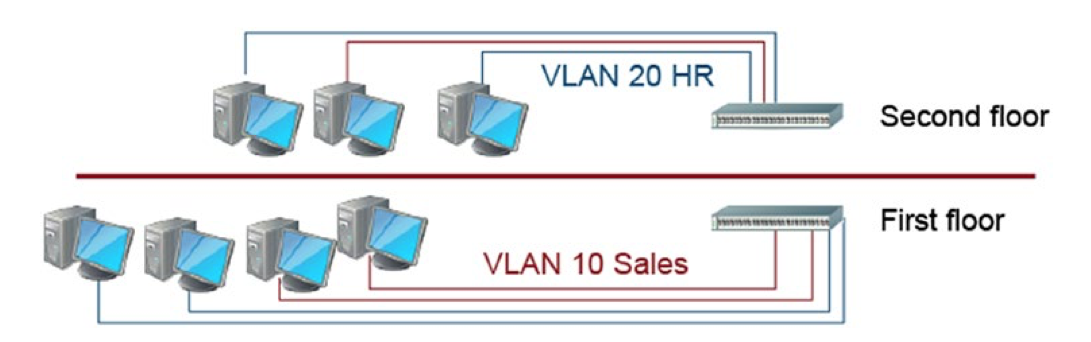
\includegraphics[width=\linewidth]{images/uploads/a_figure_08.png}
  \caption{Visuelle Darstellung der Aufteilung des Sales-Department, verbunden mittels VLAN. Quelle: \textcite{SheikhAhmedF2020CSCS}}
  \label{fig:VLAN}
\end{figure}
\bigbreak

VLANs können mittels \glqq{}Managed-Switches\grqq{} auf Basis von Port-Zuweisung oder \glqq{}Tagging\grqq{} realisiert werden. Bei Managed-Switches handelt es sich um Switches mit erweiterter Konfigurationsmöglichkeit wie etwa der gezielte Vergabe von IP-Adressen oder dem Filtering von MAC-Adressen \autocite{netgear}.
Beim portbasierten VLAN wird jedem VLAN ein spezifischer Port auf einem Switch zugewiesen, was in einem statischen VLAN resultiert. Im Gegensatz dazu wird beim tagged VLAN die Zuweisung dynamisch durchgeführt. Die Zuweisung zu einem VLAN erfolt über eine Markierung (Tag) im Frame des Nachrichtenpakets. Auf Basis des Tags kann ein Switch erkennen in welchem Segment die Kommunikation stattfindet und das Paket entsprechend weiterleiten. Jedes VLAN besitzt seine eigene Broadcast-Domäne. \autocite{ionos_digitalguide}
\bigbreak
Die Verwendung von VLANs bringt unterschiedliche Vorteile mit sich \autocite{ionos_digitalguide}:
\begin{itemize}
    \item Flexibilität\\
    Änderungen an Teilnehmern des LANs können on-demand realisiert werden.
    \item Performance\\
    Durch die Reduzierung der Broadcast-Domäne wird unnötiger Traffic vermieden und die Bandbreite minimiert.
    \item Kostenersparnis\\
    Die Verwendung von VLANs ersetzt die Installation von parallelen physischen Netzen.
\end{itemize}
\bigbreak
Der größte Vorteil liegt allerdings am Sicherheitsgewinn, wenn große Netzwerke in kleine Gruppen segmentiert werden um damit den Zugang zu beschränken. Netzwerke können so auf Basis von VLANs nach belieben strukturiert und segmentiert werden. Nur Komponenten, die sich im selben VLAN befinden, können miteinander kommunizieren, ohne an Routern oder Firewalls vorbei zu müssen. Eine Kommunikation über Netzsegemente hinweg unterliegt der Kontrolle von Firewalls. \autocite{ionos_digitalguide}
\bigbreak
Firewalls kontrollieren eingehende und ausgehende Datenpakete und regulieren den Zugriff auf Komponenten innerhalb eines Netzwerksegments auf Basis von definierten Regeln. Es wird zwischen \glqq{}Packet-Filtering\grqq{}, \glqq{}Stateful Packet-Filtering\grqq{} und \glqq{}Deep Packet-Inspection\grqq{} unterschieden. In der einfachsten Ausführung überprüft eine Firewall ein- und ausgehende Datenpakete und entscheidet auf Basis von Regeln ob die Pakete die Firewall passieren dürfen. Stateful Packet-Filtering ist eine Weiterentwicklung dieser Überprüfung und bieten ein dynamisches Paketfiltering. So kann beispielsweise der gesamten Datenverkehr blockiert werden, wenn es sich nicht Responses zu ausgehenden Requests handelt. Deep Packet-Inspection bietet eine weitere Ausbaustufe und erlaubt der Firewall den Inhalt von Paketen zu analysieren und entsprechend auf diese Inhalte zu reagieren. \autocite{SheikhAhmedF2020CSCS}
\bigbreak
Mit Hilfe von VLANs und Firewalls lassen sich Unternehmens-Netzwerke in unterschiedliche Zonen unterteilen. Die Unterteilung kann auf Basis unterschiedlicher Ansätze erfolgen \autocite{the_bristol_group_deutschland_gmbh_2021}:
\begin{itemize}
    \item Trennung auf Basis pauschaler Sicherheitszonen
    \item Trennung nach Funktion und / oder Schutzbedarf
    \item Trennung nach Gerätetyp 
    \item Trennung nach Entwicklungs- / Produktionsumgebung
\end{itemize}
\bigbreak
Bei der Trennung auf Basis pauschaler Sicherheitszonen erfolgt eine erste grobe Segmentierung des Netzwerks. Mögliche Ausprägungen sind hierbei die Trennung in \glqq{}Vertrauenswürdige Zonen\grqq{}, \glqq{}Demilitarisierte Zonen (DMZ)\grqq{} und \glqq{}Management-Zonen\grqq{}. In vertrauenswürdigen Zonen befinden sich ausschließliche IT-Systeme mit bekannter Konfiguration und bekanntem Gesundheitsstatus. DMZ sind Zonen die den Austausch mit dem Interner in kontrolliert Art und Weise sicherstellen. IT-Komponenten innerhalb von DMZ exponieren sich im Internet. Auf diese Weise können Dienste wie E-Mail, Collaboration-Tools für Externe oder Webserver für Webseiten betrieben und aus dem Internet zugänglich gemacht werden. In der Regel werden DMZ zusätzlich über Perimeter-Firewalls, die den Zugriff auf nötige IP-Adressen und Ports beschränken, nach außen hin geschützt. Managed-Zonen sind Bereiche die ausschließlich Systeme zur Bereitstellung und Verwaltung der IT-Infrastruktur beheimaten. Ein Beispiel hierfür wäre ein zentraler Active-Directory Server \autocite{iainfoulds}. 
\bigbreak
Zusätzlich zu den pauschalen Sicherheitszonen können IT-Komponenten nach Geräteart oder auszuführender Funktion etabliert werden. So bietet sich eigene Segemente für Clients, Server oder etwa IP-Telefone an. Auf Basis der Trennung nach Funktion können zusätzliche Sicherheitsmechanismen, wie beispielsweise NAC etabliert werden. Mittels NAC kann einem Client zum Beispiel der Zugang zum Client-Segment verwehrt werden, wenn der Client nicht bestimmten Anforderungen entspricht. Mit Hilfe von NAC ist es somit möglich Clients mit einem veralteten Virenschutz automatisch in ein Quarantänenetz zu stellen. 
\bigbreak
NAC bietet des Weiteren folgende Funktionen \autocite{sandata_2022}:
\begin{itemize}
    \item Lokalisierung und Identifizierung neuer Geräte im Netzwerk
    \item Authentifizierung der Geräte 
    \item Zuweisung von Rollen und Berechtigungen
    \item Prüfung der Einhaltung festgelegter Sicherheitsrichtlinien
    \item Quarantäne-Zuweisung nicht-konformer Geräte
    \item Überwachung des Verhaltens der Endgeräte im Netzwerksegment
\end{itemize}
\bigbreak
Sowohl bei der Realisierung von Netzwerksegmentierung als auch bei Verwendung von NAC ist der Schutz von Vertraulichkeit und damit einhergehend die Absicherung der übertragenen Daten und des Netzwerkverkehrs unerlässlich. Diese Tatsache wird auch von Aufsichtsbehörden erkannt. Die EBA fordert, dass beim Austausch sensibler Zahlungsdaten über das Internet eine sichere Ende-zu-Ende-Verschlüsselung zwischen den kommunizierenden Parteien eingesetzt wird (Anforderungsmatrix Nummer 218). Zu diesem Zweck soll eine starke und weithin anerkannte Verschlüsselungstechnik verwendet werden. Auch die ESMA fordert, dass Daten bei der Übertragung verschlüsselt sein müssen (Anforderungsmatrix Nummer 415). Gerade für Banken ist die sichere Übertragung von Daten, nicht nur im Bereich des Online-Bankings, unumgänglich um vertrauenswürdige Daten wie Passwörter oder Kreditkarten-Informationen zu schützen. Der vorherrschende Ansatz für die Verschlüsselung von Daten auf Transportebene ist die Verwendung von \glqq{}Transport Layer Security (TLS)\grqq{} beziehungsweise \glqq{}Secure Socket Layer (SSL)\grqq{}. \autocite{SchwenkJörg2020SuKi}

\subsubsection{Best-Practice-Ansatz: Verschlüsselung mittels SSL/TLS}
Kryptographie unterstützt bei der Wahrung der drei Sicherheitsziele \glqq{}Vertraulichkeit\grqq{}, \glqq{}Integrität\grqq{} und \glqq{}Authentizität\grqq{}. \textcite{SchwenkJörg2020SuKi} beschreibt die Erreichung der Sicherheitsziele durch Kryptografie wie folgt:
\begin{itemize}
    \item Vertraulichkeit\\
    Mit Hilfe von Verschlüsselungsalgorithmen ist es möglich, die Vertraulichkeit von Daten zu bewahren, damit nur die Besitzer eines bestimmten kryptographischen Schlüssels diese lesen können.
    \item Integrität\\
    Mit Hilfe eines gültigen \glqq{}Message Authentication Code\grqq{} (MAC) kann sichergestellt werden, dass Daten nicht verändert wurden \autocite{datatracker}. 
    \item Authentizität\\
    Die mit einer gültigen digitalen Signatur gesicherten Nachrichten können nur von der Person stammen, die den erforderlichen Schlüssel besitzt. Auf diesem Weg kann die Authentizität eines Teilnehmers gewährleistet werden. 
\end{itemize}
\bigbreak
Um die Sicherheitsziele zu gewährleisten besteht die Grundidee von SSL/TLS darin, einen verschlüsselten, transparenten und authentifizierten Kanal zur Verfügung zu stellen, über den Daten zwischen zwei Systemen zuverlässig übertragen werden können. 
\bigbreak
SSL in den Versionen 1.0 und 2.0 wurde 1994 von der Firma \glqq{}Netscape\footnote{https://isp.netscape.com}\grqq{}, zur Absicherung der Kommunikation über den Webbrowser \glqq{}Netscape Navigator\grqq{}, entwickelt. Aufgrund einiger Schwächen in Version 2.0 wurde die weitere Verwendung durch \glqq{}RFC 6176\grqq{} verboten \autocite{RFC6176}. SSL 3.0 wurde im Jahr 1996 veröffentlicht aufgrund einer Sicherheitslücke und des daraus resultierenden \glqq{}POODLE-Angriffs\grqq{} 2015 mittels \glqq{}RFC 7568\grqq{} verboten \autocite{RFC7568} \autocite{TA14-290A}. Im Jahr 1999 wurde SSL 3.1, als Upgrade auf SSL 3.0, unter der Bezeichnung TLS 1.0 veröffentlicht. TLS 1.0 wurde im Laufe der folgenden Jahre weiterentwickelt und neue Versionen im Jahr 2008 (TLS 1.2) und im Jahr 2018 (TLS 1.3) veröffentlicht. TLS 1.3 brachte große Änderungen, wie einen schnelleren Austausch von Nutzdaten und einerm verkürzten Handshake mit sich. \autocite{SchwenkJörg2020SuKi}
\bigbreak
Folgende Funktionen werden von SSL/TLS angeboten \autocite{2022C}: 
\begin{itemize}
    \item Authentifikation von Server und Client auf Basis der Verwendung von Verschlüsselungsverfahren und elektronischen Zertifikaten.
    \item Vertrauliche Client-to-Server Datenübertragung unter Verwendung eines gemeinsamen Sitzungsschlüssel.
    \item Sicherstellung der Integrität der transportierten Daten unter Verwendung des HMAC-Verfahrens \autocite{HMAC}.
    \item Komprimierung von Daten 
\end{itemize}
\bigbreak
Eine SSL/TLS-Implementierung besteht auf Client- und Serverseite aus unterschiedlichen Komponenten \autocite{SchwenkJörg2020SuKi}:
\begin{itemize}
    \item Record-Layer\\
    Dieser bildet die grundlegende Komponente über die ein sicherer Kanal realisiert wird. Der Record-Layer empfängt einen Bytestrom, den er in \glqq{}Records\grqq{} aufteilt. Diese werden einzeln verschlüsselt, authentifiziert und mittels einer Sequenznummer miteinander verknüpft. 
    \item Handshake-Protokoll\\
    Mit Hilfe dieses Protokolls werden kryptographische Algorithmen und Schlüssel zwischen Client und Server ausgehandelt. Die Nachrichten des Handshake-Protokolls werden über den Record-Layer sowohl verschlüsselt als auch unverschlüsselt übertragen. 
    \item Change-Cipher\\
    \glqq{}Change-CipherSpec-Nachrichten\grqq{} signalisieren dem Record Layer den Wechsel vom unverschlüsselten in den verschlüsselten Modus. 
    \item Alert-Protokoll\\
    Über das Alert-Protokoll werden Fehlermeldungen zwischen Client und Server ausgetauscht. 
\end{itemize}
\bigbreak
Der TLS-Handshake, in dem der Schlüsselaustausch zwischen Client und Server stattfindet, bildet das Herzstück von TLS. Mit Hilfe des Schlüsselaustausches ist es den beteiligten IT-Systemen möglich verschlüsselt zu kommunizieren. Der TLS-Handshake baut nach \glqq{}RFC 5246\grqq{} auf der \glqq{}Diffie-Hellman-Schlüsselvereinbarung\grqq{} oder dem \glqq{}RSA-basierten Schlüsseltransport\grqq{} auf \autocite{RFC5246} \autocite{RFC5990}.
\bigbreak
Der Schlüsselaustausch wird durch die beiden Nachrichten \glqq{}Certificate\grqq{} und \glqq{}ClientKeyExchange\grqq{} im Zuge des TLS-Handshakes realisiert. Hierbei sendet der Server seinen öffentlichen RSA-Schlüssel mit einem X.509-Zertifikat, in der \glqq{}Certificate\grqq{}-Nachricht an den Client \autocite{X509}. Der Client verschlüsselt daraufhin einen zufällig generierten 46-Byte-Wert zusammen mit der vom Client höchstmöglich unterstützten TLS-Version. Diese beiden Informationen bilden zusammen das \glqq{}Premaster Secret\grqq{}. Daraufhin verschlüsselt der Server das Premaster Secret mit dem öffentlichen Schlüssel des Servers und dem RSA-PKCS-Algorithmus und sendet den daraus resultierenden Chiffretext in der \glqq{}ClientKeyExchange\grqq{}-Nachricht zum Server \autocite{RSAPKCS}. Der Server wiederum kann den Chiffretext mit seinem privaten Schlüssel entschlüsseln \autocite{RFC3447}. Dieser Austausch wird von anderen beteiligten Nachrichten, wie in Abbildung \ref{fig:best-practice TLS-Handshake} ersichtlich, begleitet. \autocite{SchwenkJörg2020SuKi} 
\bigbreak
Der weitere Ablauf gestaltet sich wie folgt \autocite{SchwenkJörg2020SuKi}:
\begin{itemize}
    \item ClientHello\\
    Im Zuge der ClientHello-Nachricht werden die höchstmöglich unterstützte TLS-Version, eine Zufallszahl und eine Liste von möglichen kryptographischen Verfahren übergeben.
    \item ServerHello, Certificate, ServerHelloDone\\
    Nach Erhalt der ClientHello-Nachricht antwortet der Server mit einer Folge von Nachrichten (Entscheidung über gewähltes kryptographisches Verfahren, öffentlicher Schlüssel in Form eines X.509-Zertifikats) und schließt den Schritt mit ServerHelloDone ab. 
    \item ClientKeyExchange\\
    Der Client generiert einen zufällig Wert (PremasterSecret), verschlüsselt diesen mit dem öffentlichen Schlüssel des Servers und sendet diese Informationen an den Server.
    \item ChangeCipherSpec, Finished\\
    Der Server leitet aus dem PremasterSecret das MasterSecret ab, das als Ausgangspunkt für die Berechnung der kryptographischen Schlüssel dient. Nach Ableitung der Schlüssel kann der Client die vereinbarten Algorithmen aktivieren und den Handshake mittels ClientKeyExchange beenden. Der Server entschlüsselt die Nachricht ClientKeyExchange und leitet ebenfalls die Ableitung der Schlüssel durch. Im Anschluss daran aktiviert der Server die vereinbarten Algorithmen und beendet den Handshake mit der Nachricht ServerFinished.
\end{itemize}
\begin{figure}[H]
    \centering
  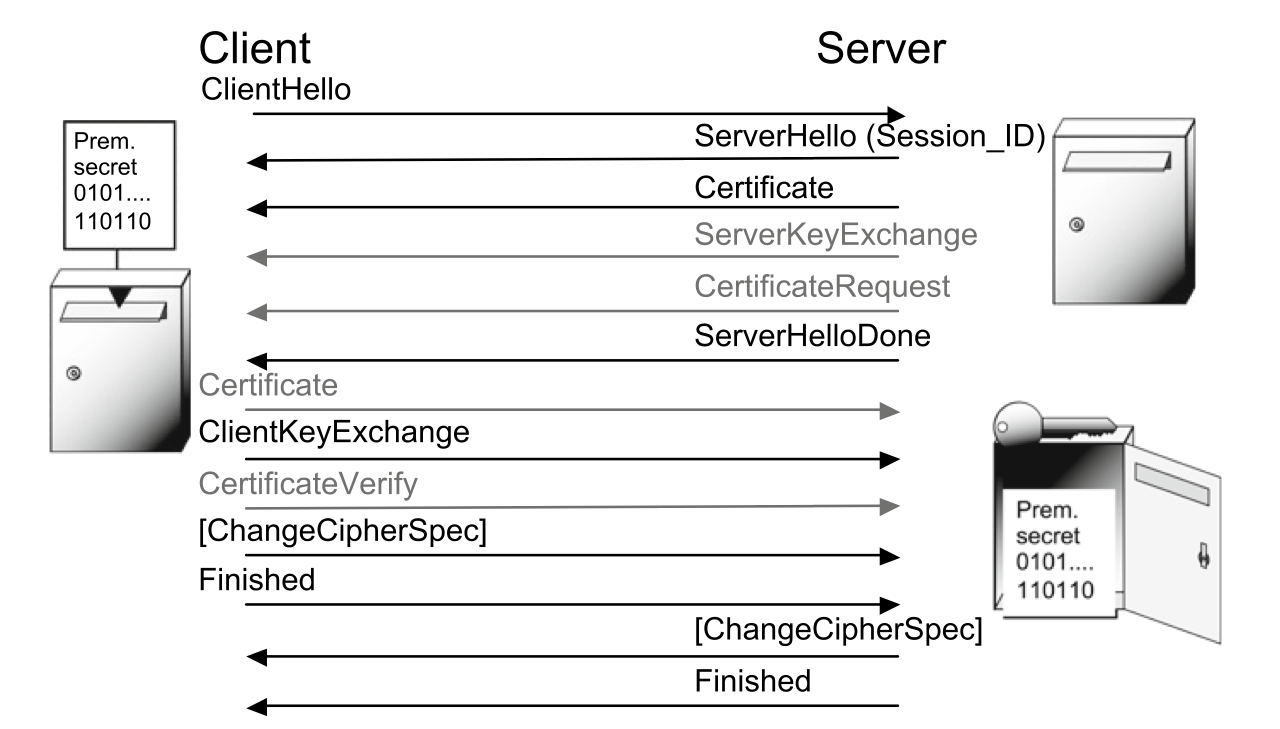
\includegraphics[scale=0.2]{images/uploads/a_figure_09.png}
  \caption{Schematische Darstellung eines TLS-Handshaktes mit RSA-basiertem Schlüsselaustausch. Quelle: \autocite{SchwenkJörg2020SuKi}}
  \label{fig:best-practice TLS-Handshake}
\end{figure}
\bigbreak
Nach erfolgreichem Handshake sind dem Server und dem Client untereinander jeweils folgende Informationen bekannt \autocite{SchwenkJörg2020SuKi}:
\begin{itemize}
    \item Die höchste vom Server und Client unterstützte TLS-Versionsnummer.
    \item Eine Ciphersuite mit einem Public-Key-Algorithmus zur Aushandlung des Premaster Secrets.
    \item Das definierte Master-Secret.
    \item Eine Session-ID.
    \item Der Verschlüsselungsschlüssel für den Datenverkehr zwischen Client und Server.
    \item Ein Schlüssel zur Generierung des MAC von Nachrichten für beide Übertragungsrichtungen.
\end{itemize}
\bigbreak
SSL/TLS wird von einer Vielzahl von Anwendungsprotokollen unterstützt und trägt somit zum Schutz der übertragenen Daten bei. Mit Hilfe von SSL/TLS kann beispielsweise eine verschlüsselte und integritätsgesicherte Verbindung für die Protokolle \glqq{}HTTP\grqq{}, \glqq{}SMTP\grqq{}, \glqq{}IMAP\grqq{}, \glqq{}FTP\grqq{} und \glqq{}Telnet\grqq{} realisiert und so den Anforderungen von Aufsichtsbehörden nachgekommen werden. \autocite{2022C}

\section{Cybersecurity-Management}
\label{Vulnerability-Management}
Die Gruppe \glqq{}Cyersecurity-Management\grqq{} vereint die Maßnahmen \glqq{}Security Incident Event Monitoring\grqq{} (SIEM), \glqq{}Log-Management\grqq{}, \glqq{}Vulnerability-Management\grqq{}, \\\glqq{}Penetration-Testing\grqq{} und \glqq{}Endpoint-Detection and Response\grqq{}. Die Gruppe beschäftigt sich mit der Erkennung von Angriffen auf IT-Systeme und dem aktiven Schutz dieser Komponenten.
\bigbreak
Der Bereich \glqq{}Cybersecurity\grqq{} deckt einen breiten Bereich an Bedrohungen und Maßnahmen ab, dem sich Banken in Österreich stellen müssen. Aufgrund der Relevanz stellen Aufsichtsbehörden unterschiedliche Anforderungen an die Cybersecurity von Banken. Die BaFin, die EBA und die FMA setzen voraus, dass Systeme für die automatische Erkennung von Anomalien und sicherheitsrelevanten Ereignissen eingeführt werden. Des Weiteren wird erwartet, dass sich Unternehmen ständig über laufende Bedrohungen und Schwachstellen des eigenen Informationsverbundes informieren, deren Relevanz prüfen und entsprechende Maßnahmen ergreifen. Aus diesem Grund haben Unternehmen ein Schwachstellenmanagement zur Erkennung, Bewertung und Behandlung von Schwachstellen zu implementieren (Anforderungsmatrix Nummer 19 und Nummer 31). Die FMA fordert des Weiteren, dass Unternehmen Maßnahmen zur Schwachstellenbeseitigung umsetzen. Unternehmen haben die Wirksamkeit der umgesetzten Maßnahmen laufend zu Überprüfung. Dies kann mittels Penetrationstests oder der Kontrolle von Logdaten durchgeführt werden (Anforderungsmatrix Nummer 265). 
\bigbreak
\subsubsection{Best-Practice-Ansatz: Aufbau Datenbasis - zentrales Logmanagement}
Ein erfolgreiches Cybersecurity-Management erfordert Kenntnisse über relevante Prozesse und Ereignisse innerhalb der IT-Struktur. Ein zur Verfügung stehendes Mittel, um Bedrohungen und Schwachstellen zu identifzieren sind Logeinträge der im Netzwerk betriebenen IT-Systeme. Eine zentrale Forderung aus dem Bereich Cybersecurity der FMA an Unternehmen, ist die regelmäßige Erfassung und Auswertung von Logdaten der im Unternehmen verwendeten IT-Systeme (Anforderungsmatrix Nummer 261). Ein zentrales Logmanagement stellt geeignete Funktionen zur Übertragung, Speicherung, Analyse und Löschung von Logdaten zur Verfügung. 
\bigbreak
In folgendem Kapitel werden die grundlegenden Bestandteile eines zentralen Logmanagements erörtert und eine mögliche Implemenierung, anhand des \glqq{}Elastic-Stacks\grqq{} (ELK-Stack), vorgestellt. \glqq{}ELK\grqq{} ist ein Akronym der im Framework enthaltenen Komponenten \glqq{}Elastic\grqq{}, \glqq{}Logstash\grqq{} und \glqq{}Kibana\grqq{} \autocite{ELK_Stack}.
\bigbreak

Für die Realisierung eines zentralen Logmanagements sind vorab unterschiedliche Überlegungen nötig: 
\begin{itemize}
    \item Welche Systeme sollen angebunden werden?\\
    Basierend auf den Betriebssystemen der jeweiligen Komponenten werden Programme zur Interpretation und Weiterleitung von Logeinträgen benötigt. 
    \item Welche Logdaten sollen übertragen werden?\\
    Werden sämtliche Logdaten eines Systems oder nur die Logdaten von bestimmten auf den Systemen betriebenen Applikationen benötigt?
    \item Wie lange sollen die Logdaten im zentralen Logmanagement gespeichert werden?\\
    Die Speicherung und Analyse von großen Mengen an Logdaten kann in einer erheblichen finanzielle Belastung resultieren.
\end{itemize}
\bigbreak
Auf Basis der genannten Überlegungen kommen unterschiedliche Komponenten für die Implementierung zum Einsatz. Am Beginn der Logmanagement-Pipeline stehen die einzelnen IT-Systeme, deren Logdaten gesammelt werden sollen. Abhängig vom Betriebssystem können die Logdaten beispielsweise mittels RSyslog\footnote{https://www.rsyslog.com}, für UNIX-Systeme, oder dem \glqq{}Windows-Event-Collector\grqq{} (WEC), für Windows Systeme, übertragen werden \autocite{WEC}. Die Logdaten werden in weiterer Folge an einen zentralen Logkollektor weitergeleitet. Für die Konstellation aus UNIX- und Windows-Systemen bietet sich Syslog-NG\footnote{https://www.syslog-ng.com} an, da dieser mit unterschiedlichen Betriebssystemen und Anwendungen kompatibel ist. Die Logdaten werden von Syslog-NG entgegengenommen und quellenabhängig zwischengespeichert. Mittels einer Analysesoftware für Logdaten, wie beispielsweise \glqq{}Filebeat\grqq{}, Bestandteil des ELK-Stacks, werden die von Syslog-NG empfangenen Logeinträge in weiterer Folge ausgelesen und weiterbearbeitet. Im Anschluss daran werden die Logdaten mittels Logstash geparsed, gefiltert, normalisiert und an Elasticsearch weitergeleitet. Elasticsearch dient der Speicherung, Indexierung, Suche und Analyse von Logeinträgen. Mittels der Weboberfläche Kibana können die gespeicherten Logdaten grafisch dargestellt werden. Abbildung \ref{fig:best-practice logmanagement} zeigt die Schematische Darstellung einer mögliche Implementierung unter Verwendung des ELK-Stacks. 

\begin{figure}[H]
    \centering
  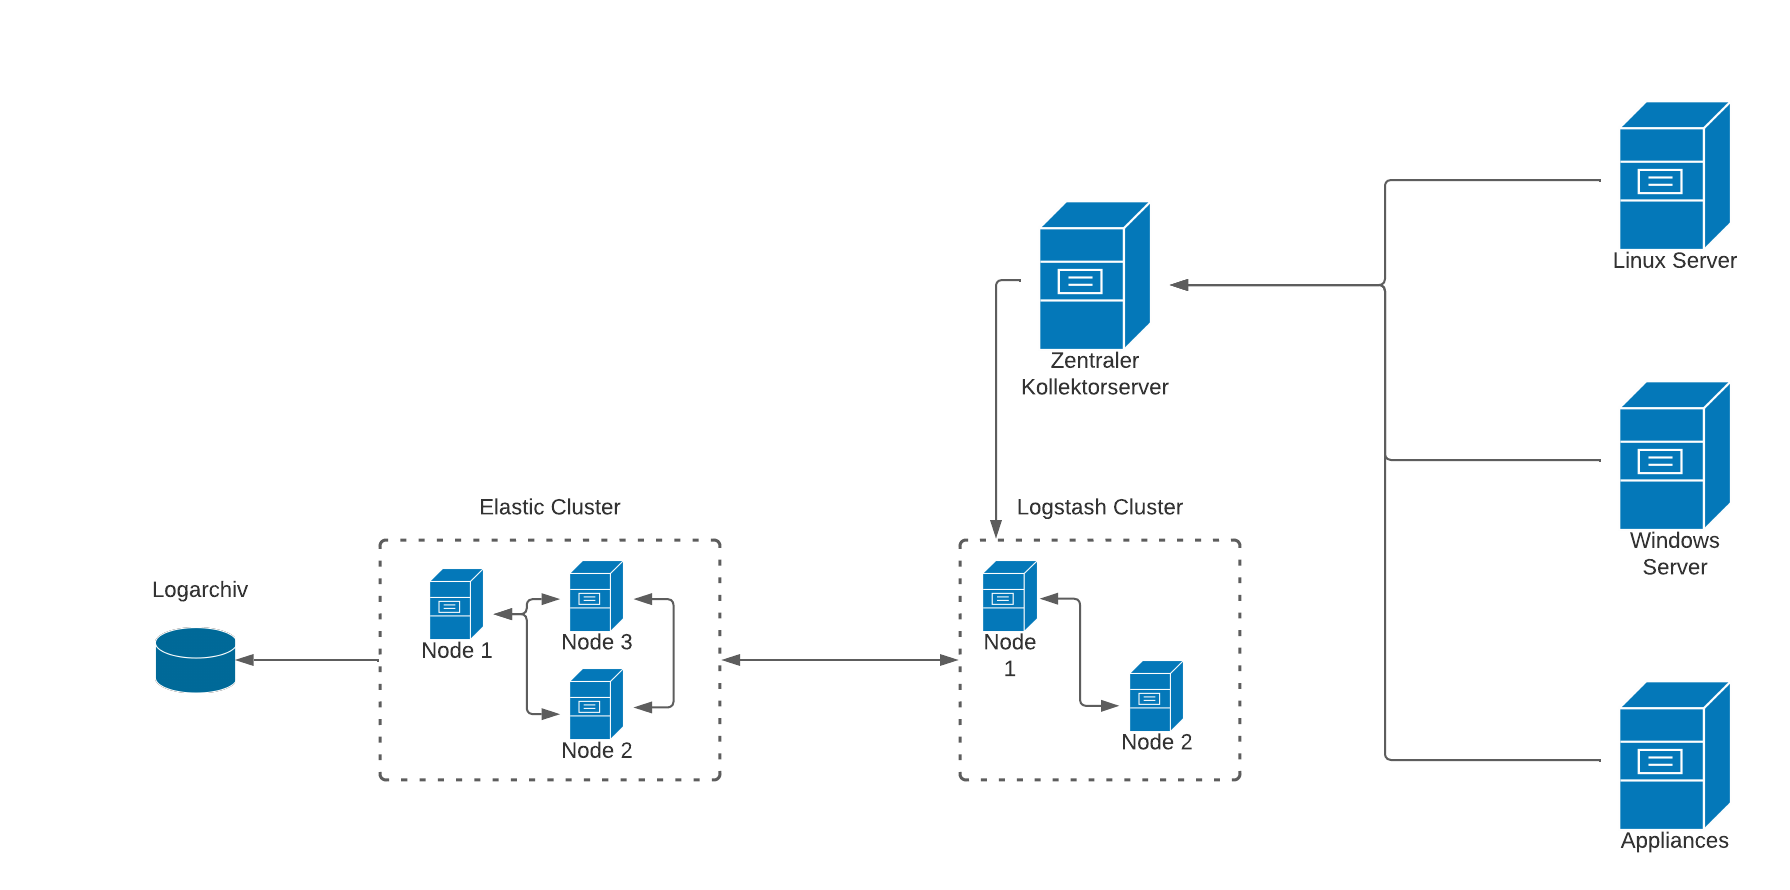
\includegraphics[scale=0.2]{images/uploads/a_figure_10.png}
  \caption{Schematische Darstellung eines zentralen Logmanagementsystems. Quelle: Eigene Darstellung, 2022}
  \label{fig:best-practice logmanagement}
\end{figure}
\bigbreak
Die Implementierung eines zentralen Logmanagementsystems kann folgende Vorteile mit sich bringen:
\begin{itemize}
    \item Erfüllung von Vorgaben der Aufsichtsbehörden.
    \item Etablierung eines zentralen Sammelpunkts für Logdaten.
    \item Möglichkeit zur zentralen Analyse sämtlicher Logdaten.
    \item Wahrung der Integrität der Logdaten (Logdaten auf den Systemen können von Angreifern gelöscht oder bearbeitet werden).
    \item Anbindung eines SIEM-Systems zur sicherheitstechnischen Analyse und Erkennung von Anomalien und Angriffsmustern.
\end{itemize}

\subsubsection{Best-Practice-Ansatz: Schwachstellen-Management}
Ein zentrales Logmanagement bietet die grundlegende Datenbasis für die Erkennung von Anomalien und Schwachstellen im IT-Netzwerk. Ein \glqq{}Security Information and Event Management\grqq{} System zentralisiert, korreliert und analysiert Daten im gesamten IT-Netzwerk in Echtzeit um etwaige Sicherheitsprobleme zu erkennen. Effizientes Log-Management ist für ein funktionierendes SIEM-System unerlässlich. Obwohl viele SIEM-Systeme aus diesem Grund auch die Funktionen eines zentralen Logmanagement-Systems bieten, wird diese Funktion aus Kostengründen häufig ausgelagert. Häufig werden SIEM-Systeme auf Basis der Menge an übertragenen Daten lizenziert und daher nur sicherheitsrelevante Logdaten vom zentralen Logmanagement in das SIEM-System importiert. Die Aufgabe eines SIEM-Systems ist es, schädliches Verhalten auf Basis vorliegender Logdaten zu identifizieren und Warnungen an die zuständigen Mitarbeiter zu senden. 
\bigbreak
Des Weiteren bieten führende SIEM-Systeme, wie etwa Splunk\footnote{https://www.splunk.com}, folgende Möglichkeiten \autocite{MehtaDeep2021SCSG}:
\begin{itemize}
    \item Überblick über relevante Events.
    \item Details zu relevanten Events.
    \item Möglichkeit zur Risikoanalyse von Systemen.
    \item Informationen über etwaige Bedrohungen.
    \item Informationen über beteiligte Prozesse bei einem Event.
    \item Definition von Usecases.
\end{itemize}
\bigbreak
SIEM-Systeme bieten die Möglichkeit eigene Usecases auf Basis von definierten Pattern zu erstellen. So besteht etwa die Möglichkeit der Implementierung einer \glqq{}Out-of-worktime Detection\grqq{} die alarmiert, falls Aktivitäten von privilegierten Accounts, außerhalb der üblichen Arbeitszeit, in den Logdaten gefunden werden. \autocite{MehtaDeep2021SCSG} 
\bigbreak
Die Implementierung eines SIEM-Systems setzt die von der EBA geforderten Maßnahmen an Banken zur Überwachung, Erkennung und Reaktion auf Sicherheitsvorfälle um. 
Häufig bieten SIEM-Systeme auch die Möglichkeit einer direkten Anbindung von Drittapplikationen, wie beispielsweise EDR-Systemen, an. EDR-Systeme bieten ähnlich wie SIEM-Systeme die Möglichkeit zur Überwachung auf Anomalien und sicherheitsrelevante Ereignisse in Echtzeit, basieren jedoch auf einem anderen Ansatz. Während ein SIEM-System auf Basis von erhaltenen Logdaten überwacht, wird bei der Überwachung mittels EDR meist ein Agent auf dem zu überwachenden IT-System installiert. 
\bigbreak
Der Agent bietet folgende Möglichkeiten:
\begin{itemize}
    \item Monitoring des zu überwachenden IT-Systems in Echtzeit.
    \item Sammeln relevanter Daten über das IT-System.
    \item Analyse der gesammelt Daten um Angriffsmuster oder Anomalien zu erkennen.
    \item Möglichkeit zur automatischen Quarantäne eines IT-Systems bei einem Sicherheits-Event.
    \item Möglichkeit zur forensischen Analyse im Zuge eines Sicherheits-Events.
\end{itemize}
\bigbreak
Ähnlich wie bei einem SIEM-System arbeiten EDR-Systeme auf Basis von Usecases. Ein bekannter Vertreter von EDR-Systemen ist Tanium.
\bigbreak
Eine weitere Möglichkeit zur Erkennung von Schwachstellen bietet das \glqq{}Vulnerability-Management\grqq{} (VuMa). Mit Hilfe von VuMa ist es möglich Sicherheitslücken in IT-Systemen und in den auf diesen Systemen laufenden Softwareprodukten zu erkennen, zu bewerten und diese zu melden. 
\bigbreak
Ein VuMa-Prozess kann in vier Schritte unterteilt werden \autocite{rapid7}:
\begin{enumerate}
    \item Schwachstellen erkennen
    \item Schwachstellen bewerten
    \item Schwachstellen behandeln
    \item Schwachstellen melden
\end{enumerate}
\bigbreak
Für die Erkennung von Schwachstellen auf IT-Systemen mittels VuMa, werden die IT-Systeme mit Hilfe eines Schwachstellenscanners überprüft. Hierfür wird das IT-Netzwerk nach zugänglichen Systemen untersucht und offene Ports oder Dienste auf den einzelnen IT-Systemen identifiziert. Es wird zwischen aktiven und passivem Scannen unterschieden. Beim aktiven Scannen interagiert der Scanner mit dem jeweiligen IT-System und bietet somit die Möglichkeit simulierte Angriffe auf das IT-System zu starten und Schwachstellen aktiv auszunutzen. Beim passiven Scannen werden detailliertere Systeminformationen gesammelt und die erhaltenen Systeminformationen in weiterer Folge mit bekannten Schwachstellen abgeglichen. Da sich das Scannen eines gesamten Netzwerkes zeitintensiv gestalten kann, können die erforderlichen Daten auch von EDR-Agents gesammelt und VuMa-Systemen zur Verfügung gestellt werden. \autocite{HaberMoreyJ2018AAV:}
\bigbreak
Werden auf einem IT-System Schwachstellen erkannt, müssen diese bewertet werden um das Risiko entsprechend behandeln zu können. VuMa-Systeme bieten meist unterschiedliche Risikobewertungen und Scores für gefundene Schwachstellen an. In der Praxis wird häufig nach dem \glqq{}Common Vulnerability Scoring System\grqq{} (CVSS) bewertet \autocite{CVSS}. Das tatsächliche Risiko einer Schwachstelle ist jedoch auch von weiteren Faktoren abhängig. 
\bigbreak
So sind folgende Punkte relevant \autocite{rapid7}:
\begin{itemize}
    \item Ist das betroffene IT-System aus dem Internet aus erreichbar?
    \item Welche Auswirkungen hat das Ausnützen der Schwachstelle auf den Betrieb?
    \item Handelt es sich um eine Schwachstelle oder ein False-positive Ergebnis?
    \item Sind noch weitere Sicherheitsmaßnahmen vorhanden die ein Ausnützen der Schwachstelle verhindern könnten?
\end{itemize}
\bigbreak
Die Behandlung einer Schwachstelle erfolgt im besten Fall durch das Einspielen eines Patches mittels Patch-Management, wie in Kapitel \ref{Patch-Management} beschrieben. Existiert noch kein Patch oder ist das System bereits aus der Wartung, können unter Umständen mitigierende Maßnahmen zur Schadensbegrenzung gesetzt werden. Ziel ist es hierbei die Wahrscheinlichkeit eines Incidents, beziehungsweise möglichen resultierenden Auswirkungen zu reduzieren. Auch die Akzeptanz eine Schwachstelle und damit einhergehend dem ausbleibenden Setzen einer Maßnahme kann einer Behandlung entsprechen. Dies kann der Fall sein, wenn die Kosten der Behebung der Schwachstelle wesentlich höher sind als die Kosten, die einem Unternehmen entstehen wenn die Schwachstelle ausgenutzt wird. \autocite{rapid7}
\bigbreak
VuMa-Systeme bieten häufig die Möglichkeit automatisierte Scans durchzuführen und im Falle einer Schwachstelle zu alarmieren. Mittels eigens konfigurierbarer Dashboards kann der aktuelle Status der IT-Systeme auch grafisch dargestellt werden. 

\subsubsection{Prävention gegenüber Angriffen}
\label{ch:penetration-tests}
Präventive Maßnahmen zur Steigerung der Sicherheit von IT-Systemen schließen das Kapitel \ref{Vulnerability-Management} ab. 
Die FMA fordert, dass umgesetzte Maßnahmen zur Schwachstellenbeseitigung regelmäßig mittels Penetration-Tests überprüft werden. 
Obwohl sich die beiden Themen VuMa und Penetration-Testing in gewissen Bereichen überschneiden, bestehen grundlegende Unterschiede. Im Zuge des VuMa wird überprüft, ob eine Schwachstelle auf einem IT-System existiert oder nicht. Die Detektion kann auf Basis von einem fehlenden Update oder beispielsweise einem nicht gesetzten Windows Registry-Key geschehen. In den meisten Fällen kann im Zuge des VuMas nicht definiert werden ob andere mitigierende Maßnahmen implementiert sind, oder nicht. Im Gegensatz dazu wird bei einem Penetration-Test versucht die Sicherheitslücke aktiv auszunutzen um zu beweisen, dass eine Schwachstelle vorhanden ist und diese ausgenutzt werden kann. \autocite{HaberMoreyJ2018AAV:} 
\bigbreak
Es existieren unterschiedliche Ansätze und Ausprägungen von Penetration-Tests:
\begin{itemize}
    \item Black-Box Test\\
    Der Tester besitzt keinerlei Informationen über die zu testende IT-Infrastruktur. 
    \item White-Box Test\\
    Der Test besitzt Informationen über die IT-Infrastruktur, vorhandene Server, Betriebssysteme, offene Ports oder verwendete Dienste. Der Sinn eines White-Box Tests liegt in der gesteigerten Effizienz und wird verwendet, wenn ein bestimmtes System oder Verfahren getestet werden soll.
    \item Grey-Box Test\\
    Hierbei handelt es sich um eine Mischung aus Black-Box Test und White-Box Test. Dem Tester sind gewisse Informationen über das zu testende System, wie beispielsweise IP-Adressen Ranges, bekannt.
\end{itemize}

%Einrücken bei Absatz verhindern
\setlength{\parindent}{0em} 

%**********************************************************************************
% Kapitel Maßnahmen und Qualitätsüberprüfung
%**********************************************************************************
\chapter{Qualitätsüberprüfung}
\section{Validierung der umgesetzten Maßnahmen}
In den vorangegangenen Kapitel wurden Maßnahmen zur Umsetzung von technischen IT-Sicherheitsanforderungen an eine Bank in Österreich untersucht. Die Frage die sich stellt ist, wie eine erfolgreiche Umsetzung dieser Maßnahmen gemessen und in weiterer Folge auditiert werden kann. 
\bigbreak
Im Zuge der Ausarbeitung haben sich folgende Möglichkeiten für die Überprüfung einer korrekten Umsetzung ergeben:
\begin{itemize}
    \item Technische Überprüfung
    \begin{itemize}
        \item Überprüfung durch interne Mechanismen\\
        Einige Produkte, mit denen Maßnahmen umgesetzt werden, bieten die Möglichkeit interner Kontrollmechanismen um die ordnungsgemäße Funktionalität des Produktes sicherzustellen. So bieten Identity-Management Systeme etwa die Möglichkeit zur Rezertifizierung von Berechtigungen oder zur Analyse ob nicht korrelierte Accounts bestehen. Auf Basis dieser Mechanismen können regelmäßige Kontrollen etabliert und auditiert werden. 
        \item Überprüfung mittels Penetration-Test\\
        Umgesetzte IT-Sicherheitsanforderungen lassen sich häufig mittels Penetration-Test überprüfen. Auf Basis unterschiedlicher Penetration-Tests, wie in Kapitel \ref{ch:penetration-tests} beschrieben, können Angriffe simuliert und die Funktionalität der IT-Sicherheitsmaßnahme überprüft werden.
        \item Überprüfung mittels Katastrophentest oder \glqq{}Business-Continuity Management\grqq{} (BCM)\\
        Ähnlich wie bei Penetration-Tests lassen sich umgesetzte Maßnahmen im Zuge eines Katastrophentests überprüfen. Häufig decken Bereiche aus dem BCM auch IT-Sicherheitsmaßnahmen ab. Im Zuge eines Katastrophentests können die Ausfallsicherheit von Systemen oder die einwandfreie Funktionalität von Backup-Prozessen überprüft werden. 
    \end{itemize}
    \item Organisatorische Überprüfung
    \begin{itemize}
        \item Überprüfung mittels Audits\\
        Interne und externe Audits sind das erste Mittel der Wahl um die Umsetzung von technischen IT-Sicherheitsmaßnahmen und deren korrekte Arbeitsweise sicherzustellen. 
        \item Überprüfung mittels internem Kontrollsystem (IKS)\\
        Auch mittels eines IKS kann die Umsetzung von Maßnahmen überprüft werden. Im Falle von Firewall-Änderungen etwa können beispielsweise periodisch Stichproben genommen und die Legitimität der Änderungen überprüft werden. 
        \item Überprüfung mittels Service-Level Agreement (SLA)\\
        Mittels vereinbarter SLAs lässt sich nicht nur die Funktionalität sondern auch die Effizienz von umgesetzten Maßnahmen überprüfen. So können SLAs Auskunft darüber geben ob kritische System-Patchens eingespielt werden und wie viel Zeit das Update in Anspruch nimmt.
    \end{itemize}
\end{itemize}
\bigbreak
Abbildung \ref{fig:matrix_ueberpruefung} zeigt die in Kapitel \ref{kap_anforderungsmatrix_abgleitete_maßnahmen} abgeleiteten IT-Sicherheitsmaßnahmen und passende Überprüfungsmethoden. 

\begin{figure}[H]
    \centering
  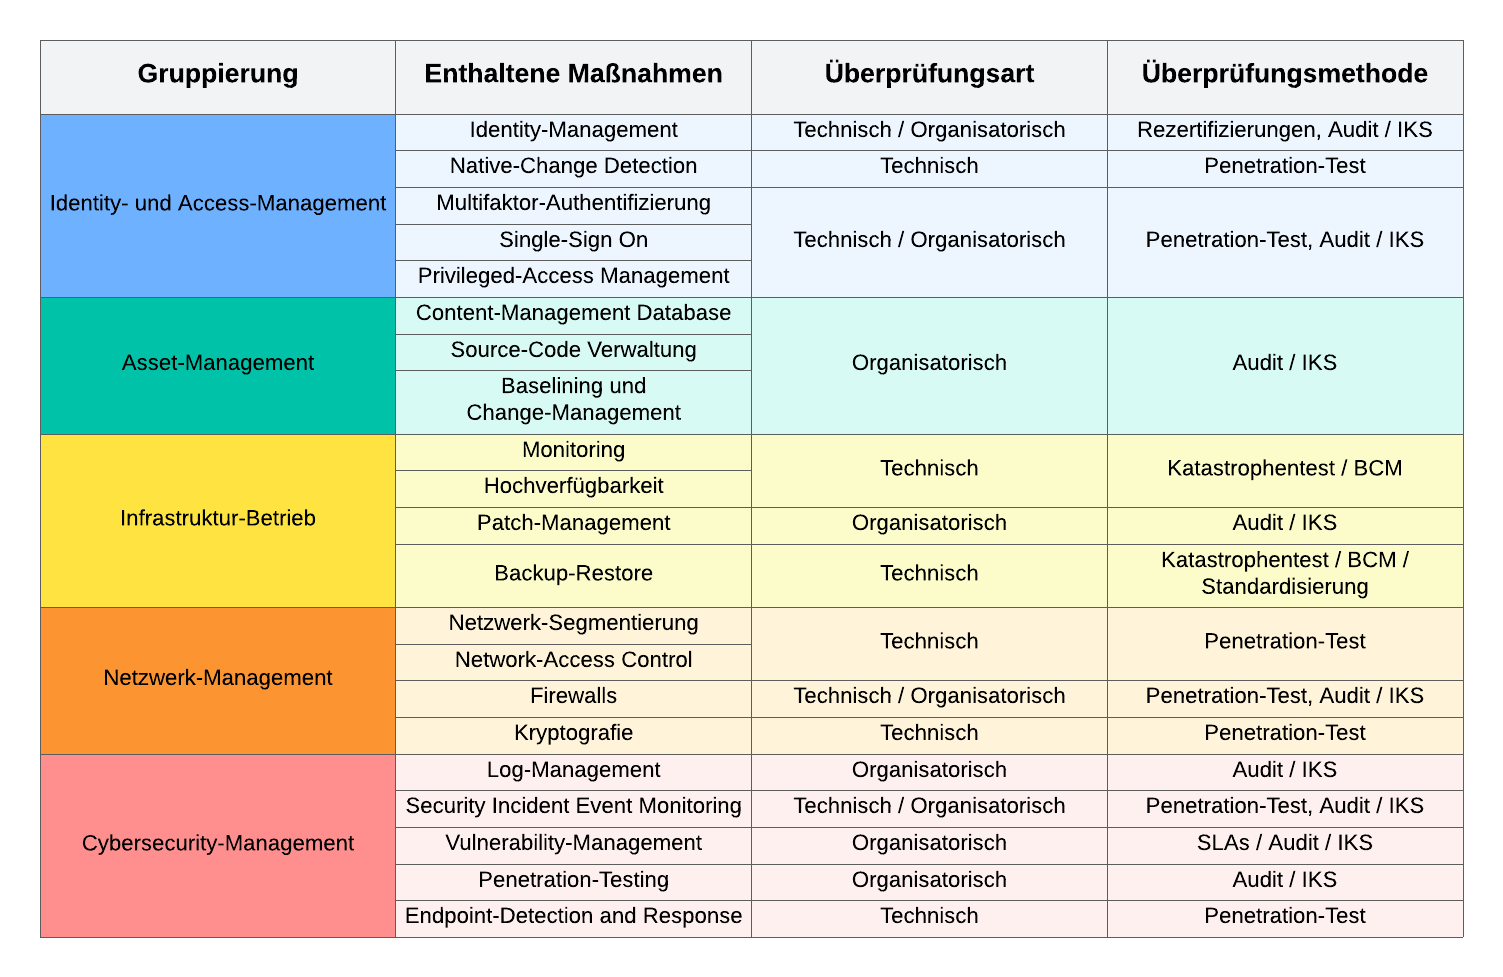
\includegraphics[width=\linewidth]{images/uploads/a_figure_16.png}
  \caption{Visuelle Darstellung der Gruppierung, enthaltenen Maßnahmen und Möglichkeit zur Überprüfung der Umsetzung. Quelle: Eigene Darstellung, 2022}
  \label{fig:matrix_ueberpruefung}
\end{figure}

\section{Vollständigkeit der Maßnahmen}
In Kapitel \ref{cha:Auswertung} wurden Maßnahmen und Best-Practice-Ansätze zur Umsetzung von technischen IT-Sicherheitsanforderungen an eine Bank in Österreich definiert und beschrieben. Zur Überprüfung, ob diese geeignet sind die Anforderungen der Aufsichtsbehörden zu erfüllen, werden die Maßnahmen und Best-Practice-Ansätze auf die \glqq{}OWASP Cyber Defense Matrix\grqq{} (CDM) angewandt \autocite{owasp_cyber_defense_matrix}. 
\bigbreak

Die CDM ist ein Open-Source-Community-Projekt unter der Leitung der OWASP\footnote{https://owasp.org} und in Abbildung \ref{fig:OWASP-CDM} dargestellt. Es handelt sich um eine zweidimensionale Matrix mit den fünf Kernfunktionen des \glqq{}NIST Cybersecurity Frameworks\grqq{} auf der X-Achse und fünf unterschiedlichen Asset-Ausprägungen auf der Y-Achse \autocite{NIST_Cybersec_Framework}. 
Das \glqq{}Nation Institute of Standards and Technology\grqq{} (NIST\footnote{https://www.nist.gov}) definiert fünf grundlegende Kernfunktionen zur Behandlung von- und zum Schutz vor Cyberangriffen, zu sehen in Abbildung \ref{fig:NIST-Framework}. 
\bigbreak
Die fünf Kernfunktionen beziehen sich auf die Zeit vor und nach einem erfolgreichen Angriff \autocite{NIST}:
\begin{itemize}
    \item Pre-incident:
    \begin{itemize}
        \item Identify\\
        Identifizierung der im Unternehmen befindlichen Assets.
        \item Protect\\
        Schutz aller im Unternehmen befindlichen Assets und/oder die Etablierung von mitigierenden Maßnahmen.
    \end{itemize}
    \item Post-incident:
    \begin{itemize}
        \item Detect\\
        Erkennen von schadhaften Aktivität auf den Assets.
        \item Respond\\
        Reaktion auf schadhafte Aktivitäten auf den Assets.
        \item Recover\\
        Wiederherstellung der jeweiligen Assets.
    \end{itemize}
\end{itemize}
\bigbreak
Die Y-Achse der CDM beschreibt fünf schützenswerte Ausprägungen von IT-Assets:
\begin{itemize}
    \item Devices\\
    Clients, Server, Storage, ...
    \item Applications\\
    Software Interaktion auf den Devices.
    \item Networks\\
    Client/Server Interaktionen, Daten die über das Netzwerk übertragen werden.
    \item Data\\
    Daten die auf den Devices gespeichert oder von diesen verarbeitet werden.
    \item Users\\
    Anwender der jeweiligen Assets.
\end{itemize}
\bigbreak
Der untere Bereich der Matrix zeigt eine Kombination aus benötigter Technologie, Menschen und relevanter Prozesse für die Adressierung der fünf Kernfunktionen. Es ist erkennbar, dass die Funktionen im linken Bereich der Matrix stark automatisiert mittels Technologie durchgeführt werden können. Die Funktionen im rechten Bereich der Matrix benötigen die Unterstützung durch Mitarbeiter und manuelles Doing. Etablierte und funktionierende Prozesse sind für alle fünf Kernfunktionen nötig.
\bigbreak
\begin{figure}[H]
    \centering
  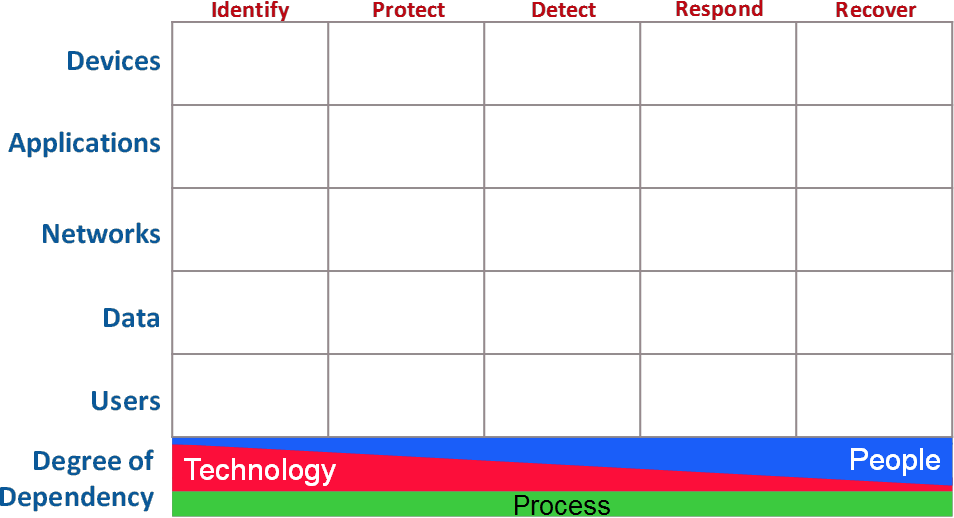
\includegraphics[width=\linewidth]{images/uploads/a_figure_12.png}
  \caption{Darstellung der CDM. Quelle: \textcite{owasp-CDM}, 2022}
  \label{fig:OWASP-CDM}
\end{figure}

\begin{figure}[H]
    \centering
  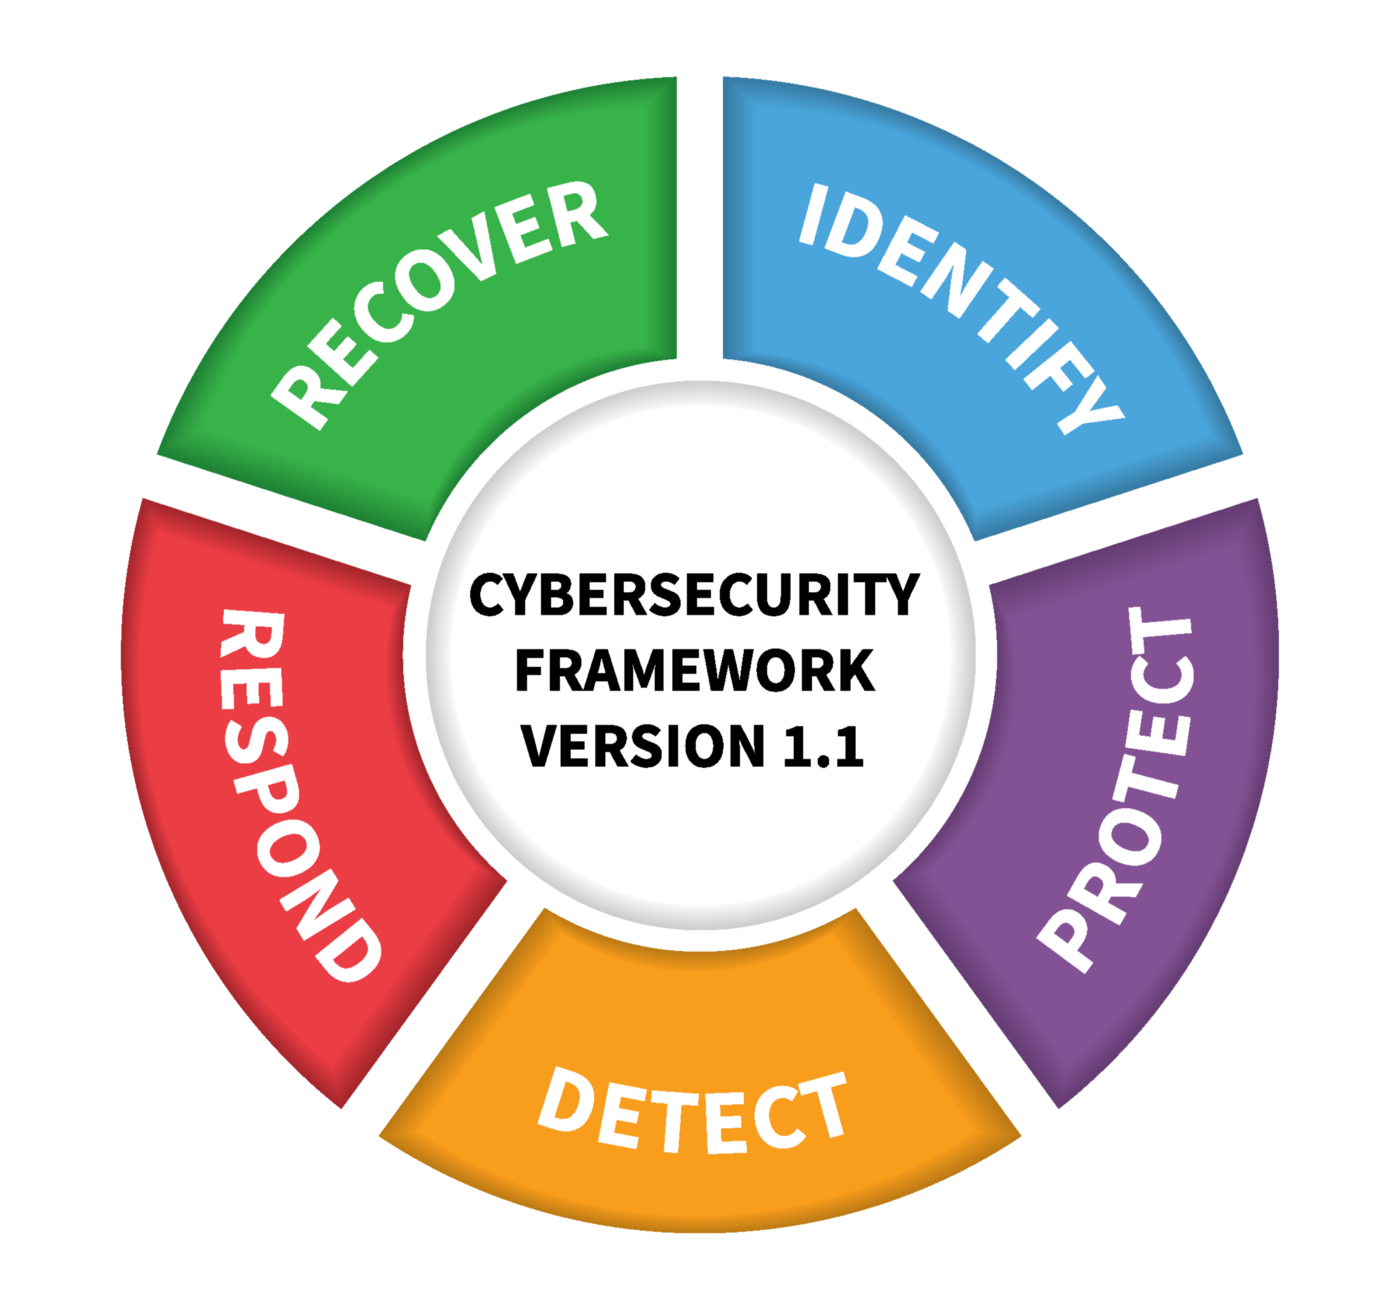
\includegraphics[scale=0.1]{images/uploads/a_figure_11.png}
  \caption{Darstellung der fünf Kernfunktionen des NIST Cybersecurity Frameworks. Quelle: \textcite{NIST}, 2022}
  \label{fig:NIST-Framework}
\end{figure}
\bigbreak
Im Zuge der Qualitätsüberprüfung werden die in Kapitel \ref{cha:Auswertung} definierten IT-Sicherheitsmaßnahmen und Best-Practice-Ansätze in die CDM eingetragen. Hierfür ist relevant in welcher Angriffsphase, welche Ausprägung von IT-Asset, mit Hilfe der jeweiligen Maßnahme geschützt werden. Dieser Vorgang lässt sich am Beispiel IAM verdeutlichen. Mit Hilfe von IAM können Anwender im Unternehmen eindeutig identifiziert werden. Des Weiteren bietet IAM Mechanismen zum Schutz der Anwender, etwa vor unerlaubter Verwendung von Benutzerdaten. Auch eine unerlaubte Verwendung von Benutzerdaten kann mittels IAM erkannt werden. Aus diesem Grund ist die Maßnahme IAM in der CDM in den Bereichen \glqq{}Users - Identify\grqq{}, \glqq{}Users - Protect\grqq{} und \glqq{}Users - Detect\grqq{} zu finden. 
\bigbreak
Es ist zu erkennen, dass die abgeleiteten Maßnahmen und Best-Practice-Ansätze einen Großteil der fünf Kernfunktionen der Matrix adressieren. Im Zuge der Ausarbeitung hat sich herausgestellt, dass die Punkte \glqq{}Identify Data\grqq{}, \glqq{}Respond Users\grqq{} und \glqq{}Recover Users\grqq{} technisch nicht realisierbar sind. Eine Identifizierung und Klassifizierung der in einem Unternehmen verwendeten Daten benötigen eine manuelle Betrachtung und kann nicht technisch realisiert werden. Die Punkte \glqq{}Detect Data\grqq{} und \glqq{}Respond Data\grqq{} wurden in den Anforderungen in Kapitel \ref{cha:regulatorische_anforderungen_und_vorgaben} und daher auch in den umzusetzenden Maßnahmen in Kapitel \ref{kap_anforderungsmatrix_abgleitete_maßnahmen} nicht betrachtet. Eine mögliche Maßnahme für \glqq{}Detect Data\grqq{} bietet die Recherche nach unternehmensrelevanten Daten im Darknet. Ein Beispiel für den Bereich \glqq{}Respond Data\grqq{} liefert die Implementierung von \glqq{}Digital Rights Management\grqq{}, der Kontrolle und dem Management von urheberrechtlich geschützten Daten. 
\bigbreak
Abbildung \ref{fig:CDM-self} zeigt die CDM, mit den in Kapitel \ref{kap_anforderungsmatrix_abgleitete_maßnahmen} abgeleiteten Maßnahmen und den in Kapitel \ref{cha:Auswertung} definierten Best-Practice-Ansätzen.  

\begin{figure}[H]
    \centering
 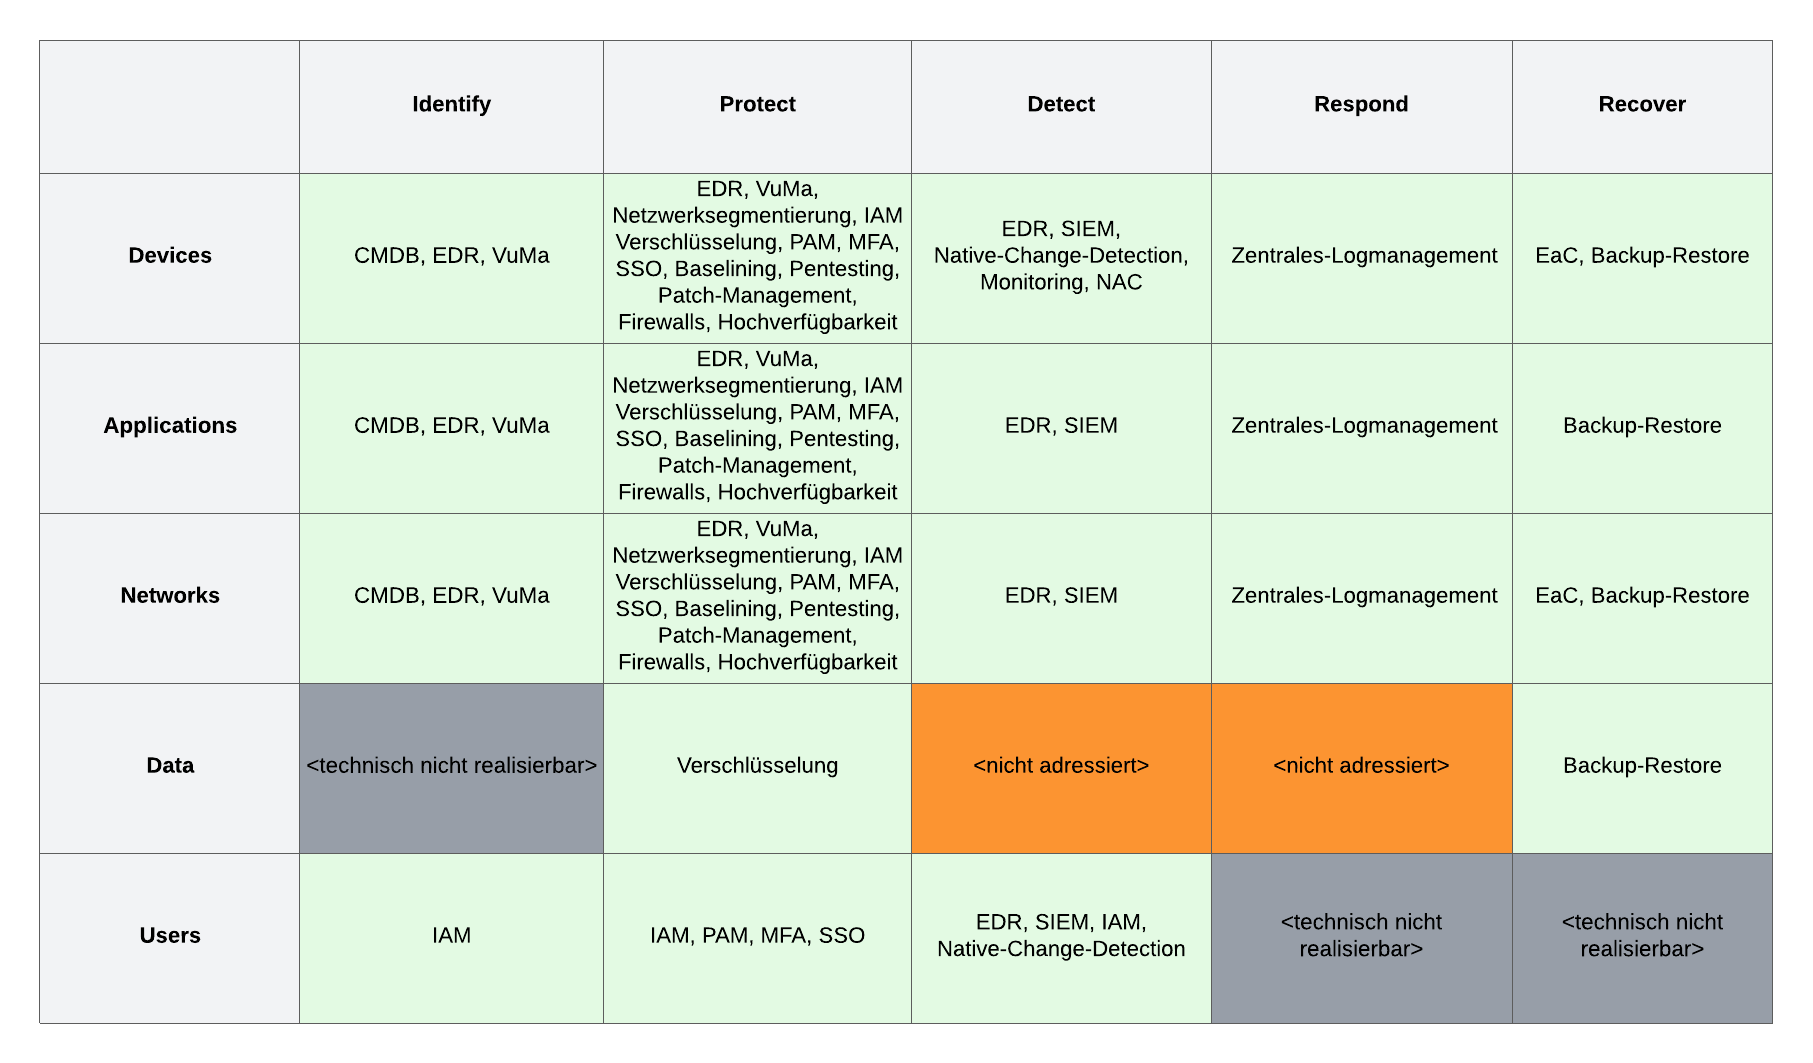
\includegraphics[width=\linewidth]{images/uploads/a_figure_14.png}
  \caption{Darstellung der CDM mit den definierten Best-Practise Ansätzen und damit einhergehenden Maßnahmen. Quelle: Eigene Darstellung, 2022}
  \label{fig:CDM-self}
\end{figure}
\bigbreak
\setlength{\parindent}{0em} 

%**********************************************************************************
% Kapitel Fazit und Zusammenfassung
%**********************************************************************************
\chapter{Fazit und Zusammenfassung}
\label{cha:fazit_und_zusammenfassung}
Die vorliegende Arbeit gibt einen Überblick über geltende IT-Sicherheitsanforderungen an eine Bank in Österreich. Im Zuge der Ausarbeitung wurden unterschiedliche regulatorische Anforderungen von Aufsichtsbehörden in einer Anforderungsmatrix dargestellt und gegliedert. In weiterer Folge wurden die relevanten Anforderungen an IT-Sicherheit untersucht und auf Basis ihrer technischen und organisatorischen Umsetzbarkeit aufgeteilt. Für die technisch umsetzbaren Anforderungen an IT-Sicherheit wurden Maßnahmen abgleitet und diese nach passenden Themengebieten gruppiert. Die einzelnen Maßnahmen jedes Themengebietes wurden beschrieben und deren Relevanz aufgezeigt. Im Zuge der Beschreibung der Maßnahmen wurden Best-Practice-Ansätze nach aktuellem Stand der Technik abgeleitet und beschrieben. Eine Qualitätsüberprüfung der abgeleiteten Best-Practice-Ansätze mittels der CDM rundet die Arbeit ab.
\bigbreak
Im Zuge der Ausarbeitung der relevanten Richtlinien hat sich gezeigt, dass 417 technische und organisatorische Anforderungen an IT-Sicherheit einer Bank in Österreich bestehen. Von diesen Anforderungen lassen sich 269 Anforderungen organisatorisch und 148 Anforderungen technisch umsetzen. Diese Aufteilung zeigt, dass das Thema IT-Sicherheit zu einem großen Teil organisatorische Maßnahmen erfordert. Die 148 technischen Anforderungen lassen sich mit Hilfe von 21 Maßnahmen umsetzen. Bei der Ableitung der Maßnahmen hat sich herausgestellt, dass sich ein Drittel der technischen Anforderungen mit der Behandlung der drei Themengebiete \glqq{}Identity-Management\grqq{}, \glqq{}Vulnerability-Management\grqq{} und \glqq{}Security Incident und Event Monitoring\grqq{} umsetzen lassen. Die technisch erforderlichen Maßnahmen sind in Tabelle \ref{table:maßnahmen_uebersicht_anzahl} aufgelistet. Im Zuge der weiteren Ausarbeitung konnten 10 Best-Practice-Ansätze definiert werden, mit deren sich die 21 erforderlichen Maßnahmen umsetzen lassen. Die Best-Practice-Ansätze und die darin enthaltenen Maßnahmen sind in Abbildung \ref{fig:bp-matrix} dargestellt. Abbildung \ref{fig:matrix_ueberpruefung} zeigt, dass eine erfolgreiche Umsetzung der Maßnahmen und damit einhergehend eine Erfüllung der technischen Anforderungen mittels technischer und organisatorischer Mittel gemessen werden kann. 
\bigbreak
Die Arbeit zeigt, dass geltende technische IT-Sicherheitsanforderungen an eine Bank in Österreich auf Basis von Best-Practice-Ansätzen erfüllt werden können. Es ist darauf zu achten, dass man sich bei der Implementierung von technischen IT-Sicherheitsmaßnahmen nicht nur auf die von Aufsichtsbehörden vorgeschrieben Anforderungen beschränken sollte. Aufsichtsbehörden geben nur ein Rahmenwerk vor, die Vollständigkeit der durch die Richtlinien abgeleiteten Maßnahmen darf nicht als gegeben angenommen werden. Schlussendlich geht es nicht darum die Anforderungen von Aufsichtsbehörden zu erfüllen, sondern die IT-Sicherheit des Unternehmens sicherstellen zu können und so gegen bösartige Angriffe gewappnet zu sein.

%%%-----------------------------------------------------------------------------
\appendix                                                               % Anhang 
%%%-----------------------------------------------------------------------------

\chapter{Peer Review}
\label{app:Peer Review}

\section{Peer 1}
\subsubsection{Fragestellung 1 - Aufsichtsbehörden}
\begin{itemize}
    \item Welchen Aufsichtsbehörden müssen Sie im Rahmen von regulatorischen Überprüfungen der Bank in Bezug auf IT-Sicherheit Rede und Antwort stehen?\\
    Antwort: Im Lead, wenn es um Prüfungen geht ist die FMA.\\
    \item Welchen Aufsichtsbehörden gegenüber sind sie im Falle eines Security-Incidents innerhalb der Bank meldepflichtig?\\
    Antwort: Security-Incidents gehen zentral an die FMA, es gibt jedoch auch EZB Meldepflichten, meines Wissens aber nur für Unternehmen, welche auch direkt von der ETB überwacht werden (Großbanken). \\
    \item Sind die in Tabelle \ref{table:uebersicht_evaluierte_literatur} aufgelisteten Aufsichtsbehörden Ihrer Meinung nach relevant für eine Bank in Österreich?\\
    Antwort: EIOPA gilt nur für Versicherungen, nicht für Banken und bildet das Pendant zu den EBA-Guidelines. Die EU ist in diesem Sinne keine Aufsichtsbehörde. Die Überwachung wird von beauftraten Behörden durchgeführt (EZB oder FMA), von der EU wird nur der Rahmen vereinbart bzw. vorgegeben. Die ENISA ist in diesem Sinne auch keine Behörde sondern eine Agentur, die im Auftrag der EU öffentliche Institutionen sowie Behörden unterstützt. \\
    \item Ist die Auflistung relevanter Aufsichtsbehörden für eine Bank in Österreich in Tabelle \ref{table:uebersicht_evaluierte_literatur} vollständig?\\
    Antwort: Ja, die Auflistung ist vollständig.\\
    \item Falls nicht, welche relevanten Aufsichtsbehörden fehlen?
\end{itemize}
\subsubsection{Fragestellung 2 - Richtlinien}
\begin{itemize}
    \item An welchen Richtlinien orientiert sich Ihr Unternehmen bei der Etablierung von IT-Sicherheitsanforderungen bzw. bei der Erstellung von Governance-Richtlinien?\\
    Antwort: Primär an Hand der Vorgaben der FMA\\
    \item Sind die in Tabelle \ref{table:uebersicht_evaluierte_literatur} aufgelisteten Richtlinien Ihrer Meinung nach relevant für eine Bank in Österreich?\\
    Antwort: Ja, die Richtlinien und Vorgaben sind relevant.\\
    \item Ist die Auflistung relevanter Richtlinien in Tabelle \ref{table:uebersicht_evaluierte_literatur} vollständig?\\
    Antwort: Ja, die Auflistung ist vollständig.\\
    \item Falls nicht, welche relevanten Richtlinien fehlen?
\end{itemize}
\bigbreak

\section{Peer 2}
\subsubsection{Fragestellung 1 - Aufsichtsbehörden}
\begin{itemize}
    \item Welchen Aufsichtsbehörden müssen Sie im Rahmen von regulatorischen Überprüfungen der Bank in Bezug auf IT-Sicherheit Rede und Antwort stehen?\\
    Antwort: FMA\\
    \item Welchen Aufsichtsbehörden gegenüber sind sie im Falle eines Security-Incidents innerhalb der Bank meldepflichtig?\\
    Antwort: FMA\\
    \item Sind die in Tabelle \ref{table:uebersicht_evaluierte_literatur} aufgelisteten Aufsichtsbehörden Ihrer Meinung nach relevant für eine Bank in Österreich?\\
    Antwort: Ja, ggf. ist die DSGVO zu ergänzen. EIOPA ist für Versicherungen relevant (Hier stellt sich die Frage, welche Produkte von der Bank angeboten werden).\\
    \item Ist die Auflistung relevanter Aufsichtsbehörden für eine Bank in Österreich in Tabelle \ref{table:uebersicht_evaluierte_literatur} vollständig?\\
    Antwort: Ja\\
    \item Falls nicht, welche relevanten Aufsichtsbehörden fehlen?
\end{itemize}
\subsubsection{Fragestellung 2 - Richtlinien}
\begin{itemize}
    \item An welchen Richtlinien orientiert sich Ihr Unternehmen bei der Etablierung von IT-Sicherheitsanforderungen bzw. bei der Erstellung von Governance-Richtlinien?\\
    Antwort: FMA\\
    \item Sind die in Tabelle \ref{table:uebersicht_evaluierte_literatur} aufgelisteten Richtlinien Ihrer Meinung nach relevant für eine Bank in Österreich?\\
    Antwort: Das BAIT-Rundschreiben ist für Österreich nicht relevant, alle anderen sehe ich als relevant an. \\
    \item Ist die Auflistung relevanter Richtlinien in Tabelle \ref{table:uebersicht_evaluierte_literatur} vollständig?\\
    Antwort: Ja\\
    \item Falls nicht, welche relevanten Richtlinien fehlen?
\end{itemize}
\bigbreak

\section{Peer 3}
\subsubsection{Fragestellung 1 - Aufsichtsbehörden}
\begin{itemize}
    \item Welchen Aufsichtsbehörden müssen Sie im Rahmen von regulatorischen Überprüfungen der Bank in Bezug auf IT-Sicherheit Rede und Antwort stehen?\\
    Antwort: Wir werden von der FMA auditiert und melden auch Security-Incidents an die FMA.\\
    \item Welchen Aufsichtsbehörden gegenüber sind sie im Falle eines Security-Incidents innerhalb der Bank meldepflichtig?\\
    Antwort: Security-Incidents werden in erster Instanz an die FMA gemeldet.\\
    \item Sind die in Tabelle \ref{table:uebersicht_evaluierte_literatur} aufgelisteten Aufsichtsbehörden Ihrer Meinung nach relevant für eine Bank in Österreich?\\
    Antwort: Für eine nationale Bank in Österreich ist die BaFin nicht relevant. Die Inhalte der BaFin werden häufig von der FMA übernommen. Die EIOPA ist für eine Bank nicht relevant. Die ENISA ist keine Aufsichtsbehörde aber natürlich relevant für Banken in Österreich.\\
    \item Ist die Auflistung relevanter Aufsichtsbehörden für eine Bank in Österreich in Tabelle \ref{table:uebersicht_evaluierte_literatur} vollständig?\\
    Antwort: Ja, ich habe nichts zu ergänzen.\\
    \item Falls nicht, welche relevanten Aufsichtsbehörden fehlen?
\end{itemize}
\subsubsection{Fragestellung 2 - Richtlinien}
\begin{itemize}
    \item An welchen Richtlinien orientiert sich Ihr Unternehmen bei der Etablierung von IT-Sicherheitsanforderungen bzw. bei der Erstellung von Governance-Richtlinien?\\
    Antwort: Wir orientieren uns hauptsächlich an den Vorgaben der FMA.\\
    \item Sind die in Tabelle \ref{table:uebersicht_evaluierte_literatur} aufgelisteten Richtlinien Ihrer Meinung nach relevant für eine Bank in Österreich?\\
    Antwort: BAIT-Rundschreiben ist nicht relevant, kann aber als Quelle herangezogen werden. Die Inhalte decken sich mit den Inhalten der FMA.\\
    \item Ist die Auflistung relevanter Richtlinien in Tabelle \ref{table:uebersicht_evaluierte_literatur} vollständig?\\
    Antwort: Aus meiner Sicht, ja.\\
    \item Falls nicht, welche relevanten Richtlinien fehlen?
\end{itemize}
\bigbreak

\chapter{Anforderungsmatrix / Git-Repository}
In diesem Git-Repository sind folgende Inhalte hinterlegt:

\begin{itemize}
    \item Latex-Source Code als .zip inklusive aller verwendeten Abbildungen und Listings
    \item Masterthesis in PDF-Form
    \item Anforderungsmatrix in Form einer Excel-Datei
    \item Archivierte Webseiten, die als Referenz verwendet wurden
\end{itemize}
\bigbreak
Link zum Repository: {\url{https://github.com/sikoqdos/MasterThesisISM2022}}: % Inhalt der CD-ROM/DVD
%%\include{back/anhang_c} % Chronologische Liste der Änderungen
%%\include{back/anhang_d} % Quelltext dieses Dokuments

%%%-----------------------------------------------------------------------------
\backmatter                          % Schlussteil (Quellenverzeichnis und dgl.)

%%%-----------------------------------------------------------------------------

\MakeBibliography % Quellenverzeichnis

%%%-----------------------------------------------------------------------------
% Messbox zur Druckkontrolle
%%%-----------------------------------------------------------------------------

%%\include{back/messbox}

%%%-----------------------------------------------------------------------------
\end{document}
%%%-----------------------------------------------------------------------------
